
\documentclass[12pt, a4paper]{article}

\usepackage[a4paper,width=150mm,top=25mm,bottom=25mm,bindingoffset=6mm]{geometry}
%\usepackage[compact]{titlesec}
\usepackage[T1]{fontenc} 	%Font 				
\usepackage[norsk]{babel}	 %Norske tegn
\usepackage[norsk]{datetime} %Dato på norsk
\usepackage[utf8]{inputenc}						
\usepackage{graphicx}       %Bilder	
\usepackage{siunitx}		%SI-enheter
%\usepackage[toc, page]{appendix} %Vedleggstillegg
\usepackage{pdfpages}		%Legge til PDF
%\usepackage{amsmath,amssymb}
%\usepackage{grffile}
%\usepackage{listings}
%\usepackage{caption}
%\usepackage[export]{adjustbox}
\usepackage{titling}		%Fancy - tittel - opplegg
%\setcounter{secnumdepth}{0}


\setlength{\textheight}{240mm} 
\setlength{\textwidth}{180mm}  
\topmargin -5mm 
\oddsidemargin -5mm


%%%%%% Forside %%%%%%

%\pretitle{%
%  \begin{center}
%  \LARGE
%  
\includegraphics[width=6cm,height=6cm]{uitlogo.png}
%}
%\posttitle{\end{center}}

\begin{document}

%\title{\\Praksis hos Norut}
%%\titlespacing*{\chapter}{0pt}{-70mm}{40pt}
%\author{Fredrik Sandhei\thanks{UiT - TEK-2000, obligatorisk rapport.}}


\begin{titlepage}

\newcommand{\HRule}{\rule{\linewidth}{0.5mm}} % Defines a new command for the horizontal lines, change thickness here

\center % Center everything on the page
 
%----------------------------------------------------------------------------------------
%	HEADING SECTIONS
%----------------------------------------------------------------------------------------

\vspace*{-3.5cm}\hspace*{-16cm}
\includegraphics{uitlogo.png}\\[3.0cm] % Include a department/university logo - this will require the graphicx package
\vspace*{-1.0cm}\textsc{\LARGE Universitetet i Tromsø}\\[2.5cm] % Name of your university/college
\textsc{\Large Praksis som valgemne}\\[0.5cm] % Major heading such as course name
\textsc{\large TEK-2000}\\[0.5cm] % Minor heading such as course title

%----------------------------------------------------------------------------------------
%	TITLE SECTION
%----------------------------------------------------------------------------------------

\HRule \\[0.4cm]
{ \huge \bfseries Rapport om praksis hos Norut}\\[0.4cm] % Title of your document
{\large \formatdate{14}{8}{2018} \hspace{1cm} - \hspace{1cm}\formatdate{10}{9}{2018}}\\[.55cm] % Date, change the \today to a set date if you want to be precise
\HRule \\[1.0 cm]

%----------------------------------------------------------------------------------------
%	AUTHOR SECTION
%----------------------------------------------------------------------------------------
\textbf{Institutt for ingeniørvitenskap og teknologi}\\
%\begin{minipage}{0.4\textwidth}
%\begin{flushleft} \large
%\emph{Student:}\\
%\textsc{Fredrik} \textsc{Sandhei} % Your name
%\end{flushleft}
%\end{minipage}
%~
%\begin{minipage}{0.4\textwidth}
%\begin{flushright} \large
%\emph{Emneansvarlig:} \\
%\textsc{Arne} \textsc{Gjengedal} % Supervisor's Name
%\end{flushright}
%\end{minipage}\\[2cm]
\hspace{-6.3cm} Fredrik Sandhei\\[.25cm] % Your name

%----------------------------------------------------------------------------------------
\begin{figure}[h!]
	\centering
	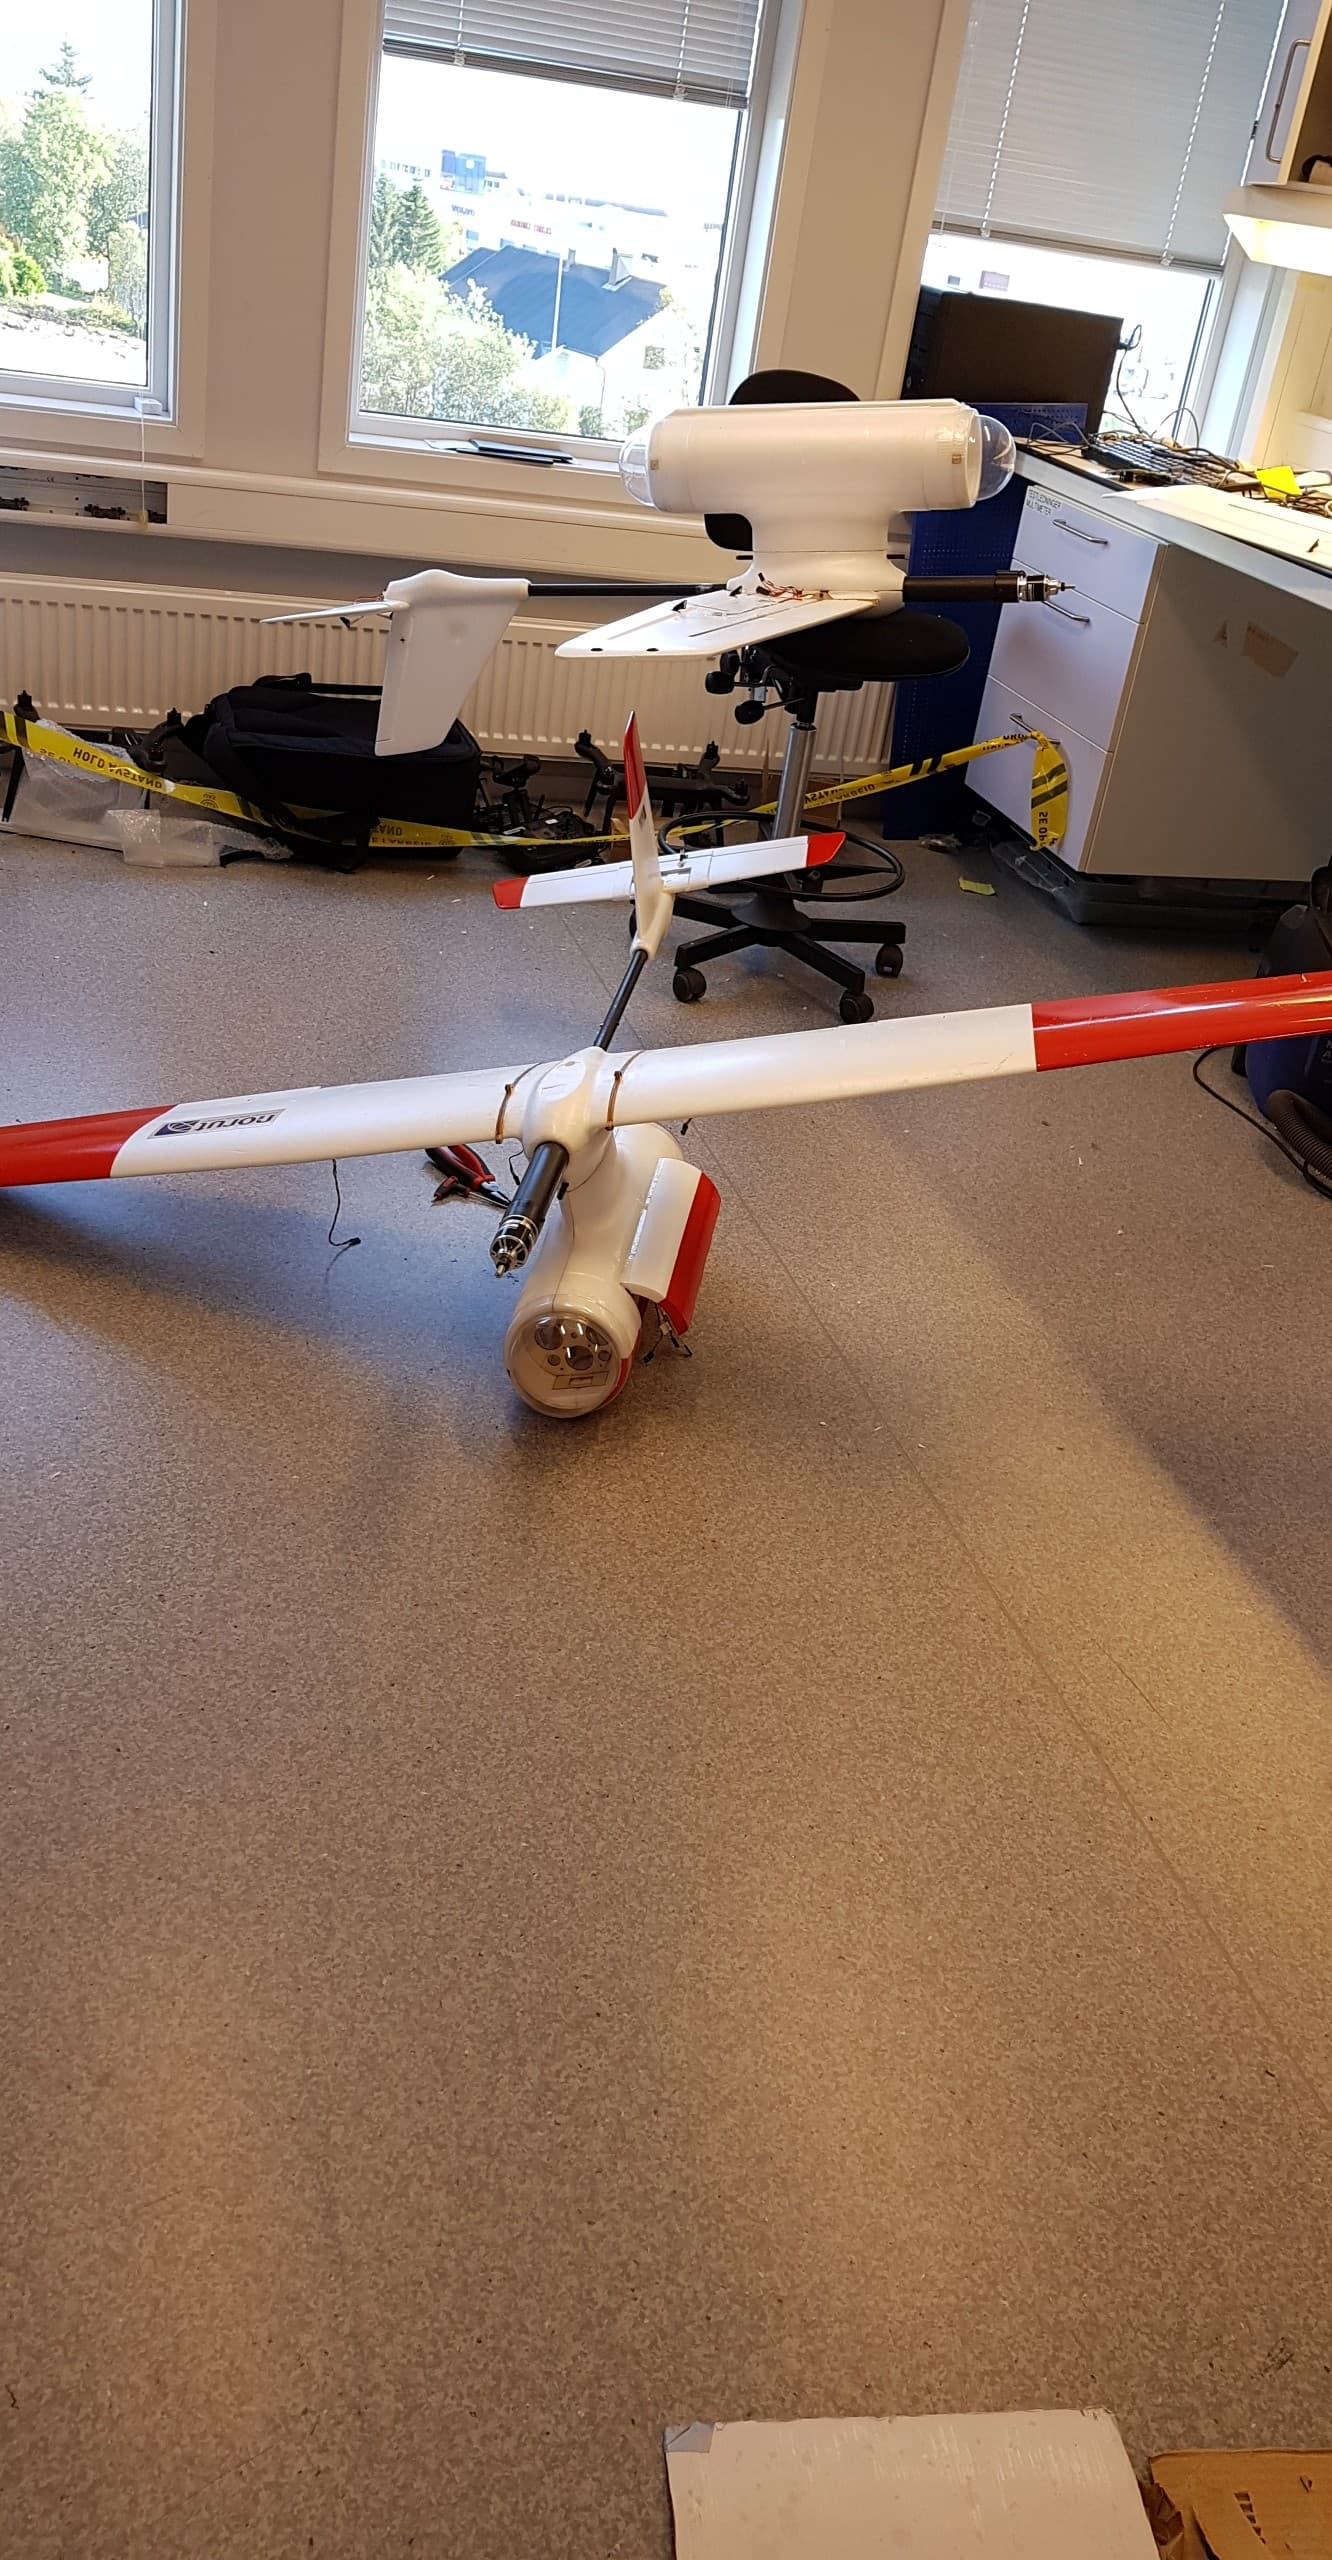
\includegraphics[width = 6cm, height = 9.3cm]{bilder/andre_fly_ferdigstilt.jpg}
\end{figure}
%----------------------------------------------------------------------------------------

\vfill % Fill the rest of the page with whitespace

\end{titlepage}
%%%%%% Slutt på forside %%%%%%
\date{\today}
%\maketitle
\clearpage

\section*{Prosjektrapport - Side 2}

\begin{tabular}{ | l | l | }
	\hline
	\textbf{Studieretning: Droneteknologi}\hspace{1.7cm} & \textbf{År: 2018} \hspace{2cm} \\
	\hline 
%	\vspace{1cm}
	\hline
	Tittel: \hspace{5cm} 			& Dato: \\
						 			& \\
	Rapport om praksis hos Norut	& Gradering: \\
    								& \\
						 			& Antall sider: \\
						 			& \\
						 			& Vedlegg: \\ \cline{1-1}
						 			& - Praksisplan \\
	Forfatter(e):		     			& - Logg av praksisperiode \\
	Fredrik Sandhei		 			& - CryoWing Observer Pilot Operating Handbook \\
									& - CryoWing Observer byggelogg \\	
						 			& - Strategi for å bestemme CryoWing\\ 
						 			& Observers egenskaper \\ 
						 			& - Attest fra Norut\\
						 			& \\						 
	\hline
	Fortrolighet: Fortrolig		 	& \\						 			
						 			& \\
						 			\hline
	Veileder:			 			& \\ 
	Arne Gjengedal 					& \\
									\hline 
	Oppdragsgiver: 		 			& Oppdragsgivers kontaktperson \\
	Norut					 		& Rune Storvold \\
						 			& \\
						 			& \\
	\hline
\end{tabular}
\vspace{.25cm}

\begin{flushleft}
	\begin{tabular}{ | l | }
		\hline
		Sammendrag: \hspace{14.7cm} \\
		\\
		Rapporten omhandler min praksisperiode hos Norut. Hovedoppgaven min var \\ å bygge og dokumentere tre fly av typen CryoWing Observer. \\
		Ting gikk ikke helt som planlagt. Dermed ble bare to fly bygd og jeg fikk ikke\\
		muligheten til å gjennomføre testflygning og dermed flyene.
		Jeg har likevel lært mye \\ praktisk som 
		jeg kan ta videre i utdannelsen og arbeidslivet.
		\\
		\hline
		Stikkord: \\ Praksis, Norut, CryoWing Observer, droneteknologi\\ \\ \\ \\
		\hline
	\end{tabular}
\end{flushleft}

\clearpage


\section{Sammendrag}
Denne rapporten beskriver min praksisperiode hos UAV-avdelingen til Norut i Tromsø. Jeg gjennomførte praksisperioden min i begynnelsen av høstsemesteret 2018, hvor jeg var 4 uker i strekk hos Norut. \\

Hovedoppgaven jeg fikk var å produsere tre CryoWing Observer fixed-wings, der én av disse skulle være en RC-trainer, mens de to andre skulle utstyres med autopilotsystem inkludert andre periferier. I tillegg til dette skulle jeg dokumentere flyenes luftdyktighet ved å testfly dem og fylle ut flyets egenskaper.\\

Flyene ble bygd ved å følge en bruksanvisning. Da jeg hadde svært lite erfaring med bygging fra før, var det å følge bruksanvisningen slavisk. \\

Mangel på opplæring og uregelmessig oppfølging samt lite tilgjengelighet på utstyr og personell gjorde at arbeidet tok lengre tid enn forventet. Dagene ble dermed stressende i og med at tre fly skulle bygges. Det ble besluttet at det var nok å få bygget to og i hvert fall få testflydd det ene flyet. \\

To fly ble ferdigbygd og det ene ble testflydd. Dessverre havarerte flyet i testflygning. Det var ikke mulighet å gjøre mer, da jeg ble ferdig med praksisen den samme dagen. \\

Til tross for det jeg oppfatter som stressende dager, har jeg lært mye, men på den ``harde måten''. Jeg har fått lært mye innenfor teknisk med tanke på struktur, komposittmaterialer i form av epoxy-lim og anvendelse av teori fra studiet. Hovedoppgaven har vært svært relevant med utdannelsen, og har gitt meg en god smak på hva som kan være i vente når jeg kommer ut i arbeidslivet som droneingeniør. \\

\newpage

\section{Forord}
TEK-2000 `Praksis som valgemne' er et av de tre emnene jeg har valgt for 5.semesteret mitt på 3.året i droneteknologi. Emnet går ut på at studenten skal ha en praksis hos en bedrift som er passende til utdannelsen. Praksisplassen må fylle kriterier fra emneansvarlig på bedriftens relevans til utdannelsen. \\

Jeg søkte praksis hos to plasser, Luftfartstilsynet og Norut. Begge er relevante på hver sin måte. Jeg fikk innpass hos begge, men på grunn av lokalitet og mest relevanse valgte jeg Norut.\\

Denne rapporten beskriver min praksisperiode i UAV-avdelingen til Norut i Tromsø, hovedoppgaven min, og hvordan jeg har løst denne, inkludert mine refleksjoner av perioden. Da rapporten inneholder vedlegg som er stemplet fortrolig av Norut, er rapporten fortrolig, og skal leses av sensor og emneansvarlig. \\ 

Takk til Norut i Forskningsparken i Tromsø for at jeg fikk muligheten til å kunne gjennomføre praksisen min hos dem. Takk til forskningssjef Rune Storvold og resten av UAV-avdelingen for min tid der. Takk til UiT for å gi muligheten til studentene å ta dette emnet, og spesielt takk til emneansvarlige som godkjente praksisen min hos Norut og har gitt veiledning til utarbeidingen av denne rapporten. \\[7cm]
%\vspace{7cm}
Tromsø, \today \\[.5cm]

\begin{flushleft}
	\begin{tabular}{@{}p{.5in}p{4in}@{}}
	Signatur: & \hspace{.5cm}\textbf{Fredrik Sandhei} \\
			  & \hrulefill \\
	\end{tabular}

\end{flushleft}
\clearpage

\begin{minipage}[b]{1\linewidth}
	\tableofcontents
	\vspace{.5cm}
\end{minipage}
\begin{minipage}[b]{1\linewidth}
	\listoffigures
\end{minipage}
\clearpage

\section{Innledning}
I begynnelsen av høstsemesteret 2018 begynte jeg en praksisperiode hos Norut i samsvar med emnet TEK-2000, hvor jeg var i fire uker. Min oppgave for denne perioden har vært å bygge tre fly på bestilling av Norut. I tillegg til dette har jeg vært litt i flere områder på avdelingen for ubemannede luftfartøy (UAV-avdelingen) og hjulpet litt rundt med reparasjonsarbeid og papirarbeid. Formålet med denne praksisperioden var å få et innblikk i hvordan et typisk arbeidsliv til en ingeniør kan være. \\

I løpet av vårsemesteret 2018 var jeg innom Norut og snakket med Rune Storvold om muligheten for praksis. Han fortalte at det var arbeid som de hadde ønsket å få gjort, men som de selv ikke hadde kapasitet til for øyeblikket. Jeg har hatt interesse for modellflyging helt siden barndommen, men har aldri bygget et før, bortsett fra et par multirotorer. Jeg var samtidig spent og gledet meg til å få gjøre dette. Tanken å få bruke det man har lært opp til nå gjennom studiet syntes jeg virke svært spennende. Erfaringene mine hos Norut kommer jeg til å ta med meg videre i utdannelsen min og det kommende arbeidslivet. 

%Norut er et nasjonalt forsknings- og innovasjonsselskap som produserer anvendbar, nordområderelevant kunnskap innen teknologi og samfunnsvitenskap. Norut er kjent for å bruke ubemannet luftfartøy (UAV) til deres vitenskapelige formål. De har brukt UAV lenge før det ble mer eller mindre nasjonalt anerkjent av Luftfartstilsynet.\\


%Rune Storvold er forskningssjef og leder av UAV-avdelingen hos Norut og var ansvarlig for min praksisperiode i Norut. Praksisen foregår i 20 dager. Jeg avtalte med Rune Storvold at praksisen skulle gjennomføres i et kontinuerlig kjør. Praksisen begynte i uke 33 og avsluttet i uke 37.\\


%En arbeidsdag hos Norut går fra 08:00 - 15:00. Etter endt praksis skal en rapport leveres inn fra studenten om praksisperioden.\\
%Prosjektoppgaven min hos Norut var å produsere tre fly av typen Cryowing Observer, der to av disse skulle utstyres med GPS-systemer og andre periferier. Den tredje skulle være en RC-trainer, med bare radiolink (RC-link). Dette var arbeid som Norut hadde ønsket å få gjort, men som de ikke selv hadde kapasitet til å få gjennomført.\\ 


%Da det var travle tider da jeg begynte praksisperioden min hos Norut, ble det mye slik at det var lite hjelp å få, og oppfølgingen av byggingen var dårlig. Byggeprosessen tok derfor lengre tid enn forventet. Det ble dermed besluttet at det var nok å bygge to fly og i hvert fall få testet det ene flyet og dokumentert dette før endt praksisperiode. Selv om jeg ikke fikk dokumentert det ene flyet, da dette gikk i bakken på testflygingen, synes Rune Storvold at arbeidet gjort hos Norut var tilfredsstillende for hva som ble mulig å gjennomføre i løpet av en 4-ukers periode.\\


%En attest for praksisperioden ligger som vedlegg til denne rapporten fra Norut, inkludert en logg over arbeidsdagene der jeg har loggført hva som ble gjort dag for dag. I tillegg ligger ved papirene som jeg måtte lage til testflyging og beskrivelsen av praksisperioden som måtte leveres inn før begynnelse av praksisperioden.

%FÅ RETNINGSLINJENE FOR RAPPORTEN...
%Beskriv emnet, hensikten og hva som må gjøres
%FÅ MAL FRA EMNEANSVARLIG

\newpage
\section{Om arbeidsplassen}
\subsection{Norut}
Norut Northern Research Institute AS, eller Norut, er et nasjonalt forsknings- og innovasjonsselskap som produserer anvendbar, nordområderelevant kunnskap innen teknologi og samfunnsvitenskap. Selskapet ble dannet i 1992 og er majoritetseid av Universitetet i Tromsø. Norut har kontor i Alta, Bodø, Harstad og Bardu, med hovedkontor i Tromsø. \\

Som en forskningsvirksomhet er Norut delt inn i ulike forskningsområder. Disse områdene strekker fra arktisk teknologi til urfolk.
Norut er kjent for å bruke ubemannet luftfartøy (UAV) til deres vitenskapelige formål, spesielt satellitt- og fjernmålingsteknologi.  De har brukt UAV lenge før det ble mer eller mindre nasjonalt anerkjent av Luftfartstilsynet.\\

Bruk av UAV er en forholdsvis ny plattform for datainnhenting. Å bruke UAV er betydeligere billigere med tanke på materialer og ressurser enn ved bruk av bemannet luftfart. Ved at ingen personer er om bord luftfartøyet ved flyging, reduseres risikoen for personskade, og oppdrag som kan være utfordrende å gjøre blir forenklet med bruk av UAV. \\

Da det foreløpig ikke er satt ordentlige standarder til drift av ubemannet luftfart, har Norut egne rutiner på drift og vedlikehold som de har selv satt. På grunn av Noruts erfaring med UAV, bidrar Norut med ressurser og opplæring av studentene på droneteknologi-utdanningen hos UiT. \\

Norut har en flåte av luftfartøy med kombinasjon av multirotorer og fixed-wing fly. Flyene er døpt til CryoWing, der noen av skrogene er importert fra Slovakia, og avionikken, motorsystem og annet er montert av Norut. Enkelte fly og multirotorer er byggesett som Norut har satt sammen eller hyllevarer. De ulike fartøyene brukes til ulike formål der det er passende, deriblant landmåling og fjernmåling.\\
\newpage

\subsection{Noe av flåten}
\begin{figure}[hpbt]
	\centering
	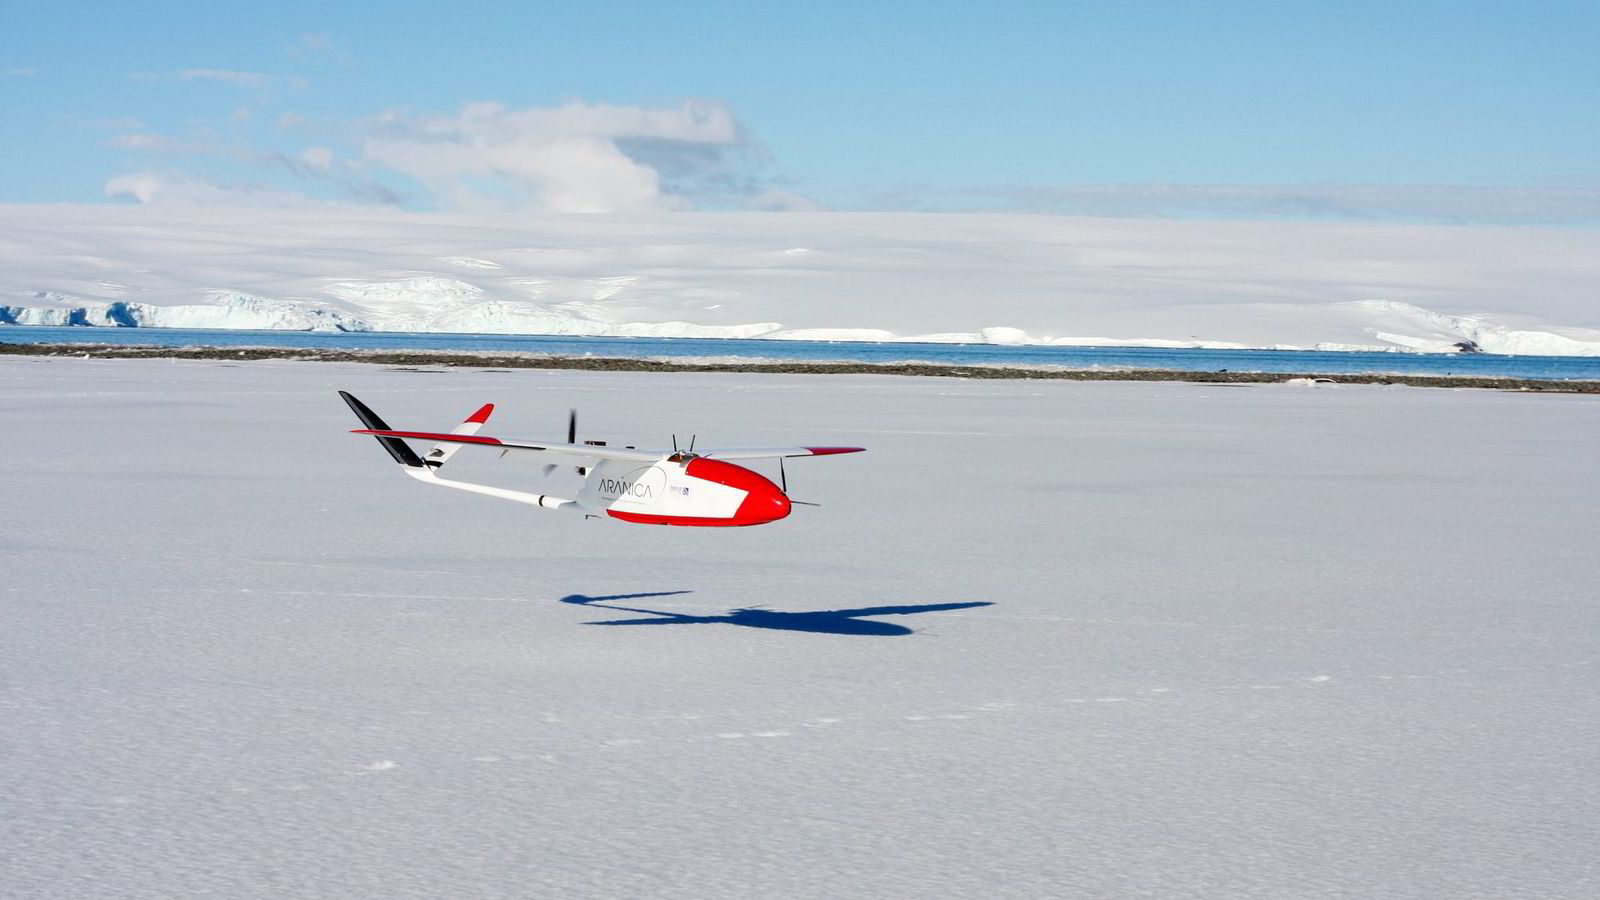
\includegraphics[width=.6\textwidth, height=9cm]{bilder/CryoWing_Explorer.jpeg}
	\caption[CryoWing Explorer]{Noruts pragd - CryoWing Explorer}
\end{figure}

\begin{figure}[h!]
	\centering
	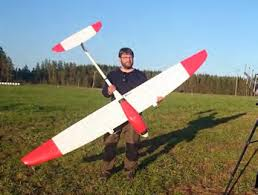
\includegraphics[width=.6\textwidth, height=9cm]{bilder/CryoWing_Scout.jpeg}
	\caption{CryoWing Scout}
\end{figure}

\newpage

\begin{figure}[hpbt]
	\centering
	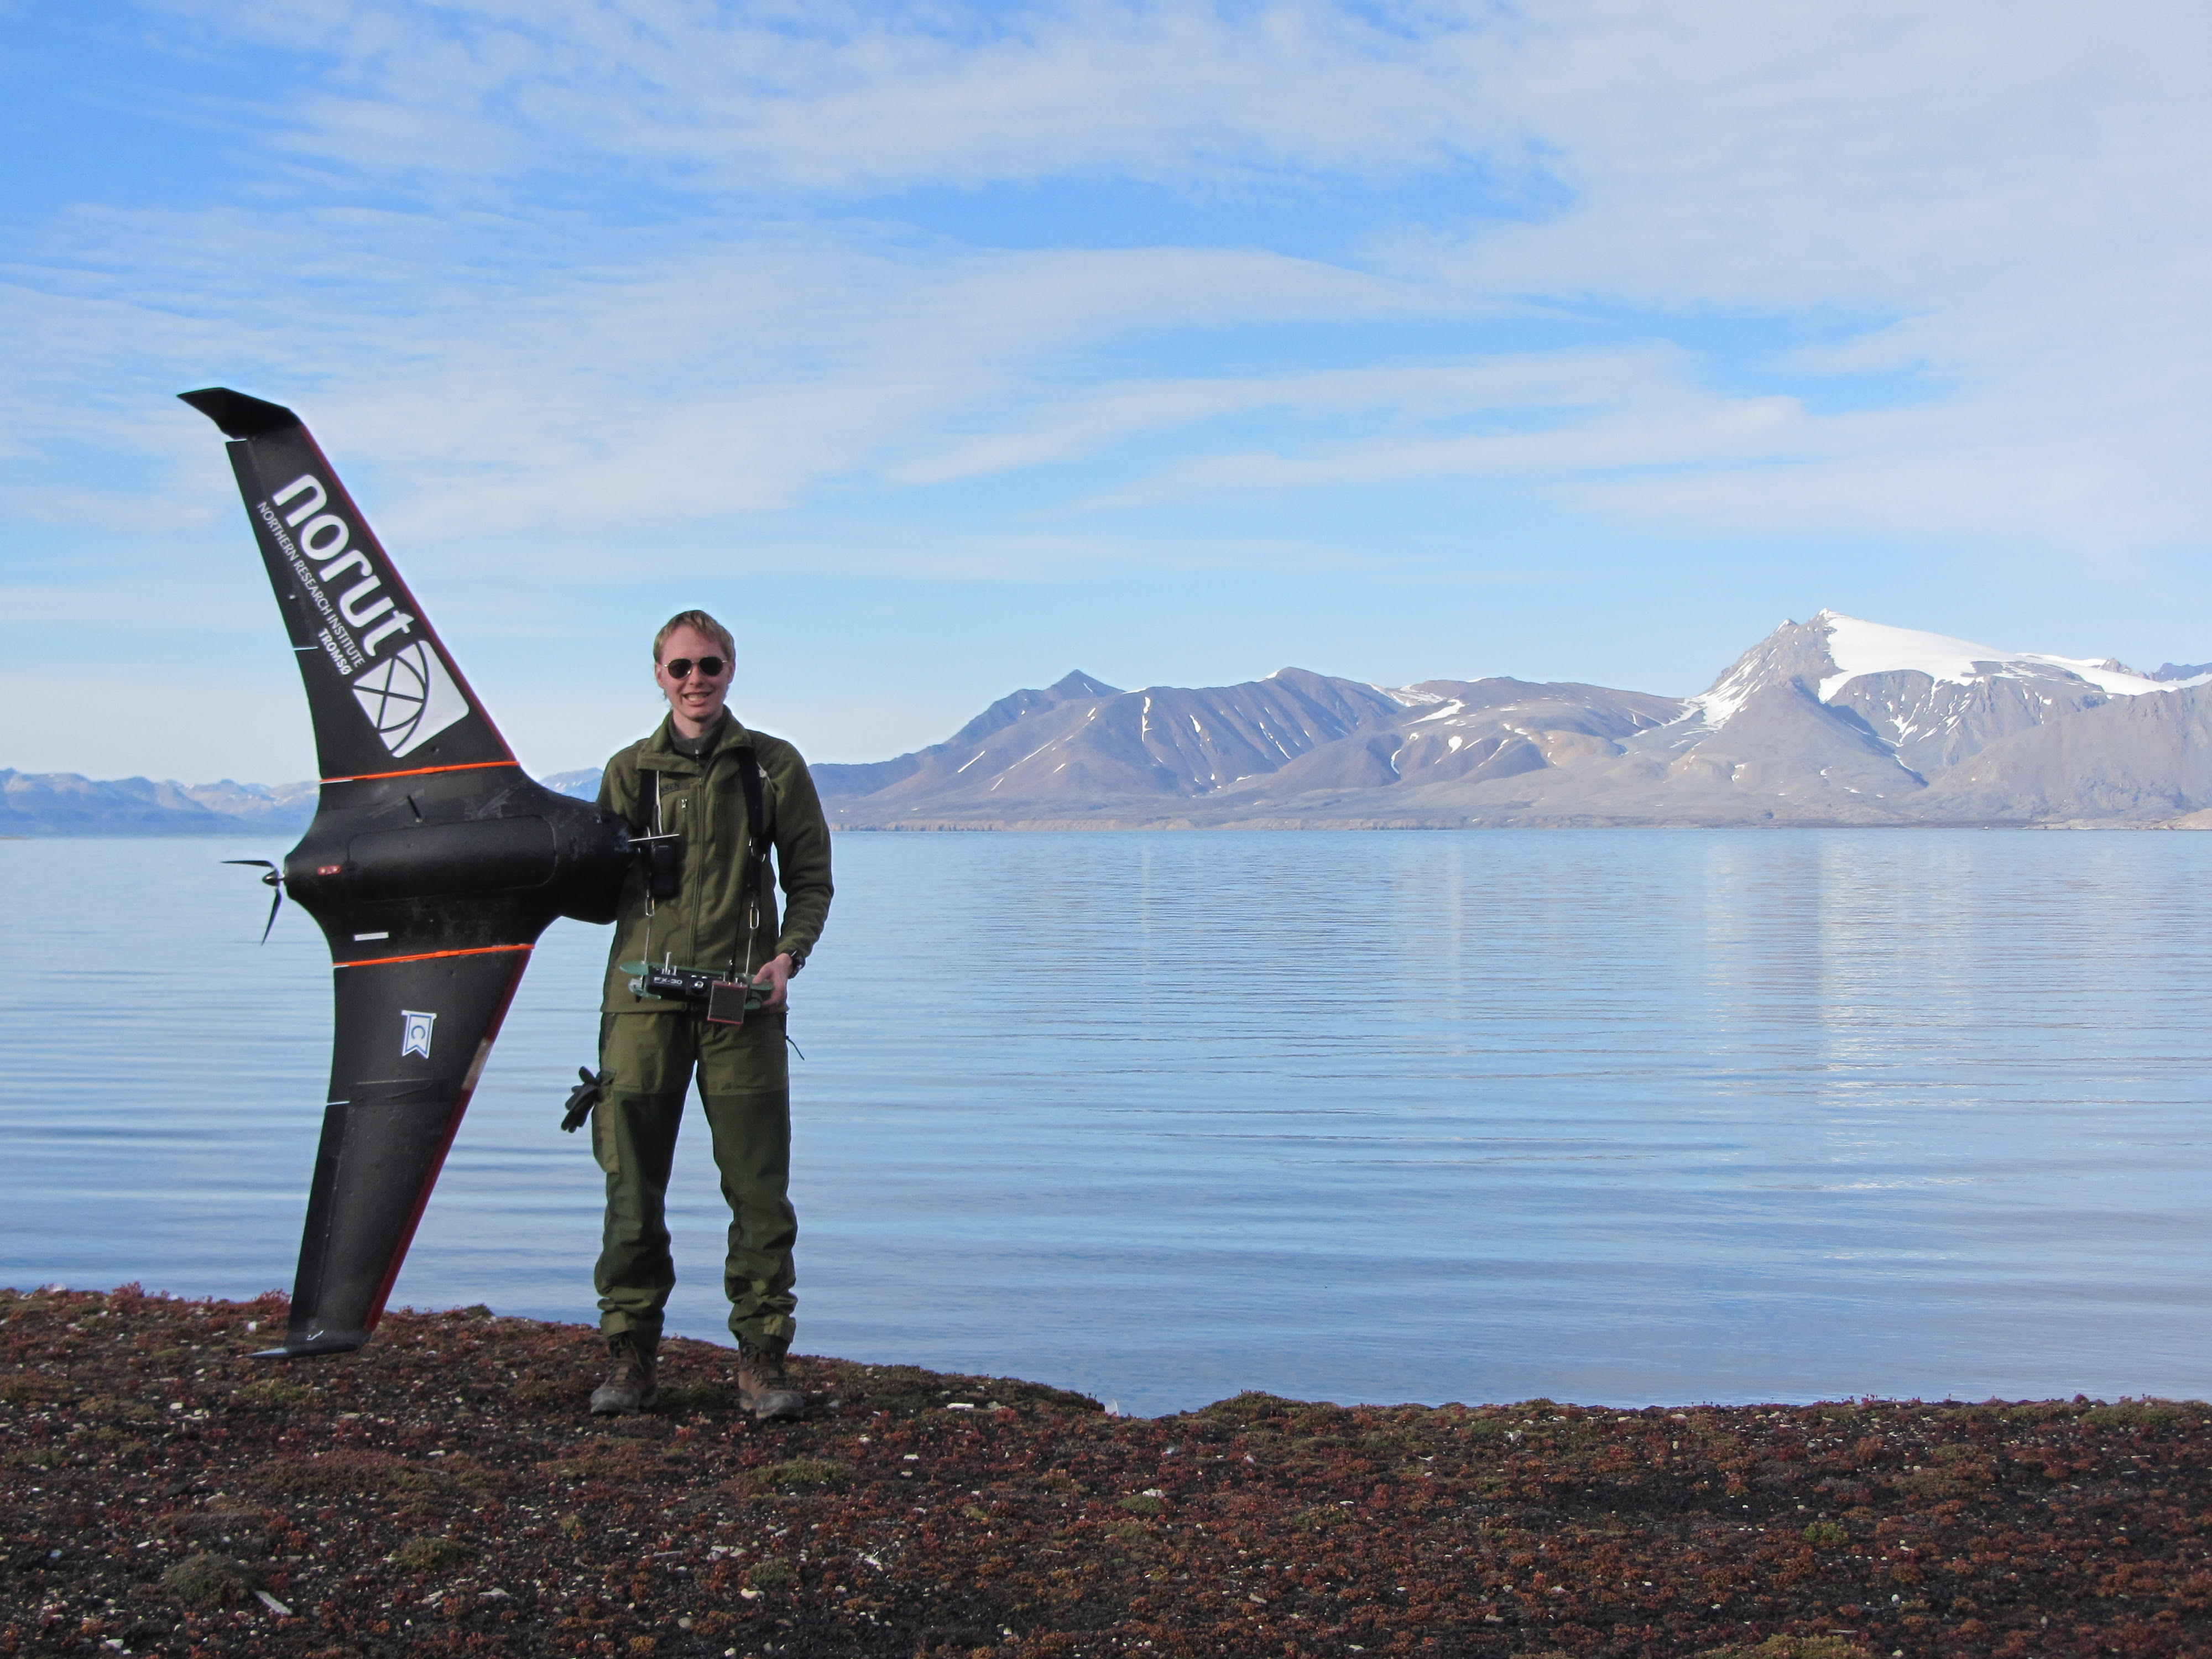
\includegraphics[width=.6\textwidth, height=9cm]{bilder/SkyWalker_X8.jpg}
	\caption{SkyWalker X8}
\end{figure}

\begin{figure}[h!]
	\centering
	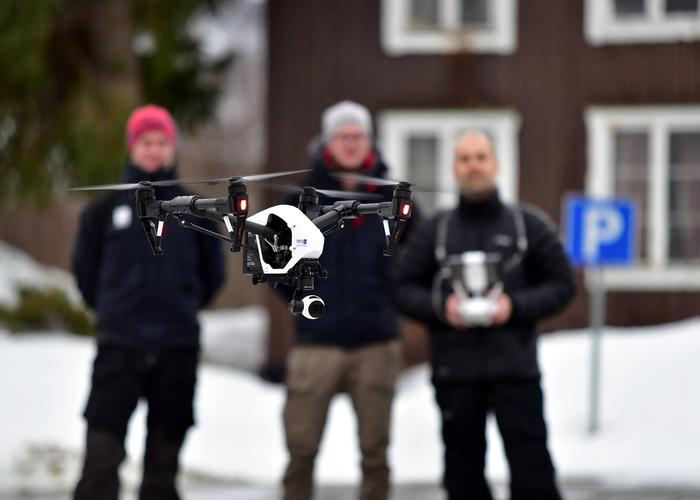
\includegraphics[width = .6\textwidth, height = 9cm]{bilder/Dji_inspire.jpg}
	\caption{DJI Inspire}
\end{figure}


\newpage
\section{Hendelsesforløp}
%Kort om hver uke. Få frem meningen med alt
%Få beskrevet arbeidsoppgavene, forhåpentligvis ei liste 
%som blir oversiktlig.
%Litt frem og tilbake på hva jeg driver med
\subsection{Første uke og prosjekt}
\subsubsection{Backlog og GIS}
%Back log av flight plans
%Flyoperativ avdeling 
%Avdelingsmøte
Den første dagen begynte med omvisning av bedriften og jeg fikk hilse på de andre som var tilstede. Deretter ble jeg satt rett i arbeid med backlog av tidligere flight plan inn i det GIS-baserte loggsystemet deres. \\
Typisk metodikk innen luftfart synes å være ``learning by doing''. Poenget er det å prøve ut for seg selv og ta utgangspunkt i eksempler som er gitt. Jeg så dermed på tidligere logger som var ført og fulgte deres oppsett.\\
En flight log er et skjema som beskriver en flyoperasjon. Loggen skal minimum inneholde flytype, tidspunkt for take-off, landing, tid i lufta, drivstoff brukt, hvilke luftfartsinstanser man har vært i kontakt med om noe, vær og så videre. 

%Bilde av loggskjema
\begin{figure}[ht]
	\centering
	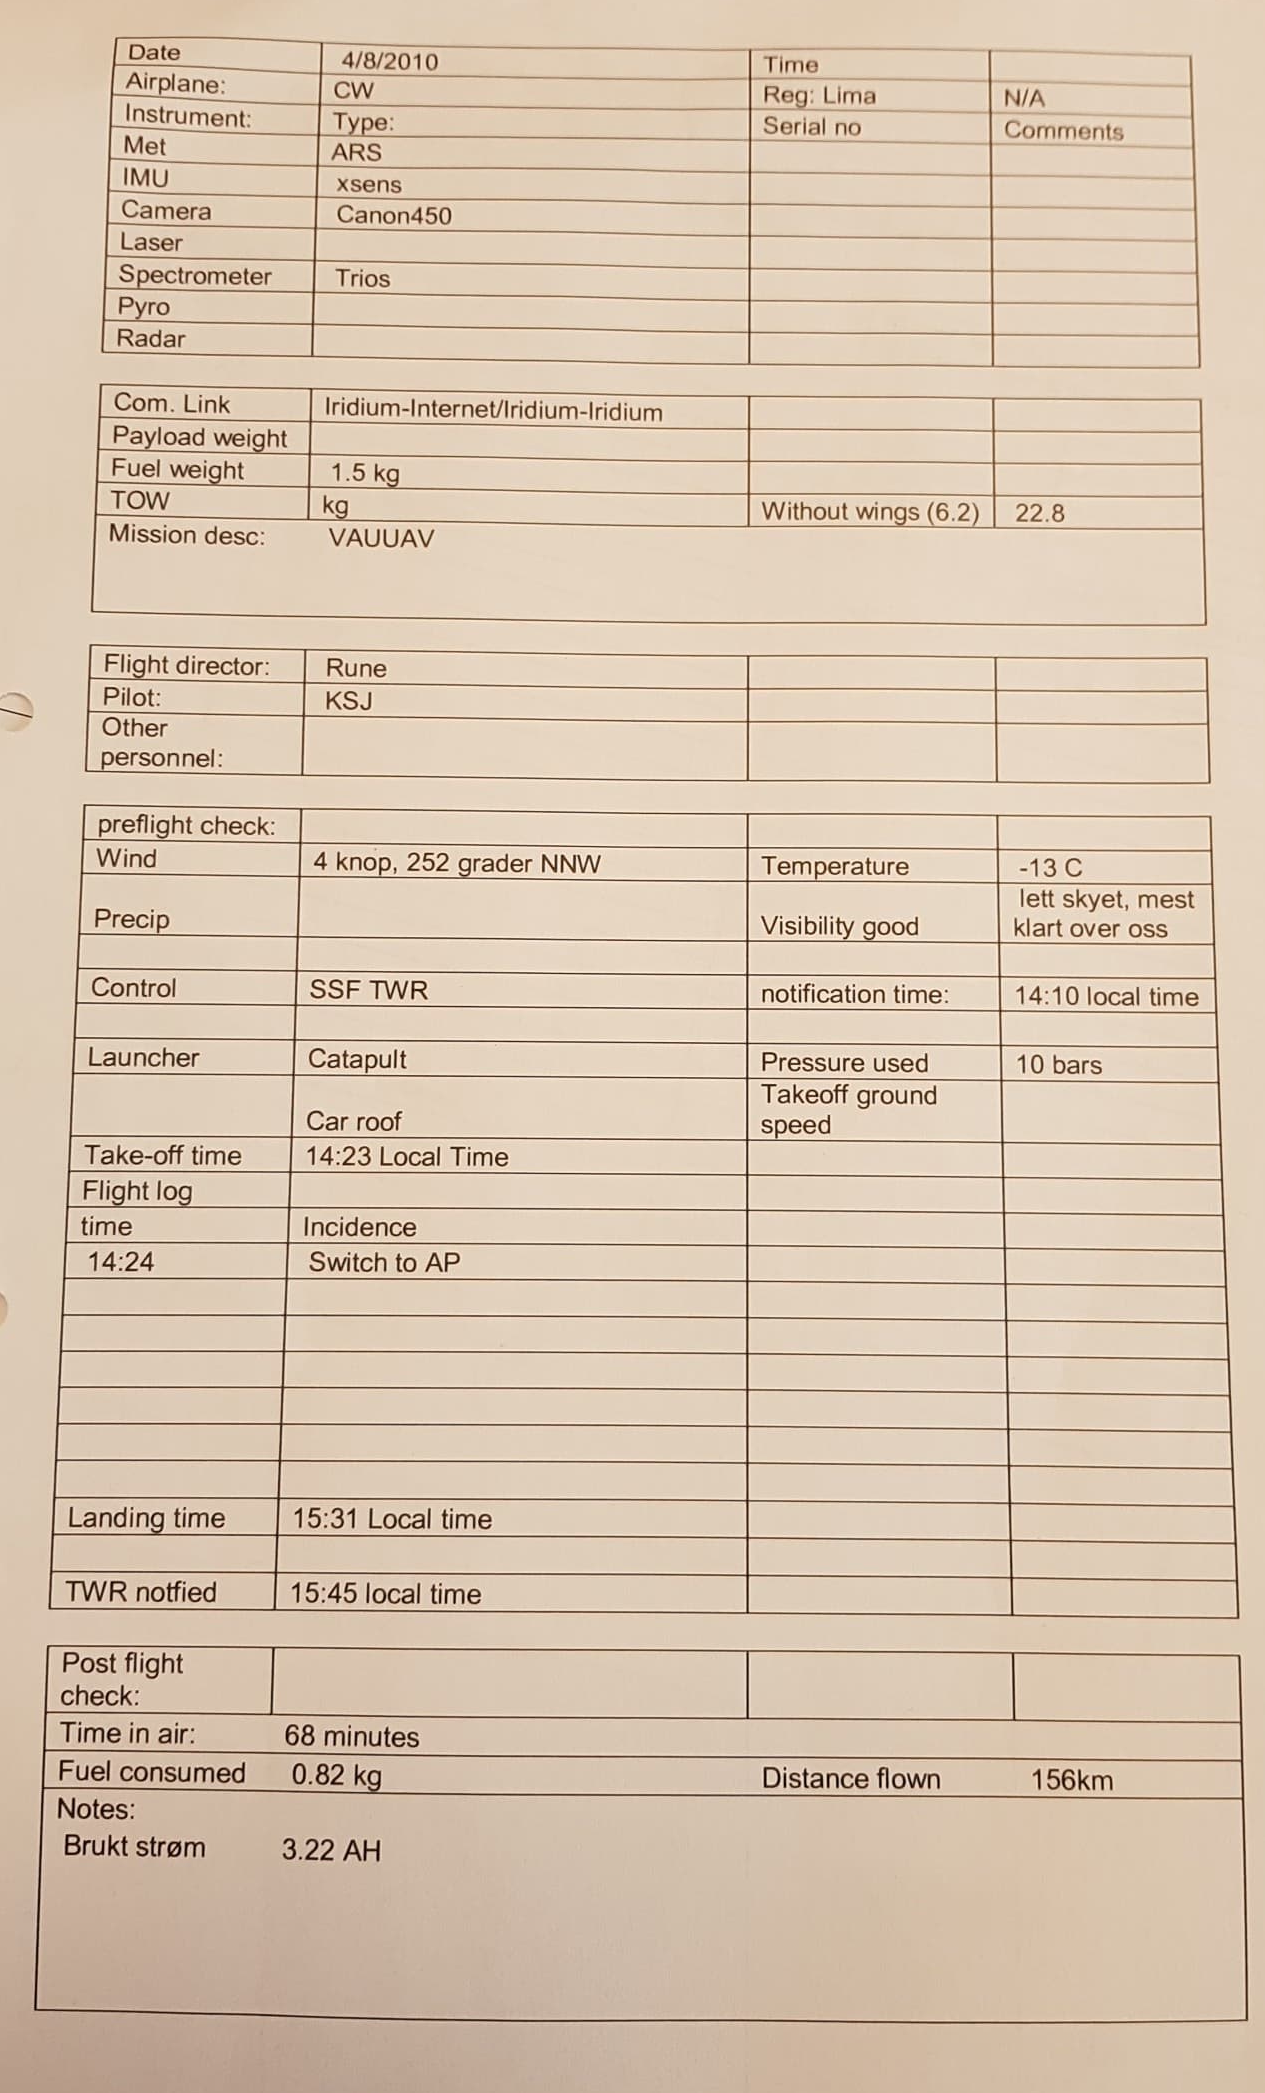
\includegraphics[height= 10cm, width=0.5\textwidth]{bilder/flightlogNorut.png}
		\caption[Loggskjema]{Typisk opplegg av loggskjema til Norut. Skjemaet skal inneholde nødvendig informasjon om flighten som kan brukes til gjennomgang for neste flight. }
\end{figure}

\newpage
Mesteparten av den første dagen gikk til backlog samt at jeg fikk delta på et avdelingsmøte.\\
\subsubsection{Forberedelse til byggeprosjekt}
Dag 2 fikk jeg et prosjekt utdelt som jeg skulle fokusere på i de neste ukene. Prosjektet gikk ut på bygging og testflyvning av tre fly av typen Cryowing Observer. \\
Flyene skulle også dokumenteres luftdyktigheten på. Det vil si at det må dokumenteres hvor god stand disse er til å følge kravene Norut har satt for sikker flyvning. Til forberedelse av prosjektet ble jeg bedt om å legge opp en plan for hvordan jeg vil finne de ulike egenskapene til flyene, som skal dokumenteres i en såkalt POH (Pilot's Operating Handbook). I denne POH'en skulle jeg blant annet finne følgende opplysninger gjennom testflygninger: 
\begin{itemize}
	\item Cruise speed
	\item Stall speed
	\begin{itemize}
		\item Flap up power off
		\item Half flap power off
		\item Full flap power off	
	\end{itemize}
	\item Standard empty weight
	\item Maximal Take Off Weight (MTOW)
	\item Useful load
	\item Wing loading
	\item Power loading
	\item Minimal battery capacity
\end{itemize}
Oppsettet jeg lagde for testflygningen er vedlagt til rapporten, se vedlegg. 
Selve byggingen av luftfartøyene kunne ikke begynne før uke 2, da delene måtte hentes opp fra Bodø. \\ 
\newpage
I mellomtiden drev jeg med reparasjonsarbeid på et av Noruts multirotorer som havarerte. Nye rammer måtte settes på, elektroniske fartskontrollere måtte kobles opp og konfigureres og mer. Da jeg har drevet med noe bygging av multirotorer fra hobbybasis, samt fått teoretisk kompetanse fra emnene på studiet, gikk mye av arbeidet bra. Konfigurasjonene som Norut bruker (se bildene under), var litt nytt, men prinsippet var det samme som på hobbyprosjektene mine. \\

\begin{figure}[ht]
	\centering
	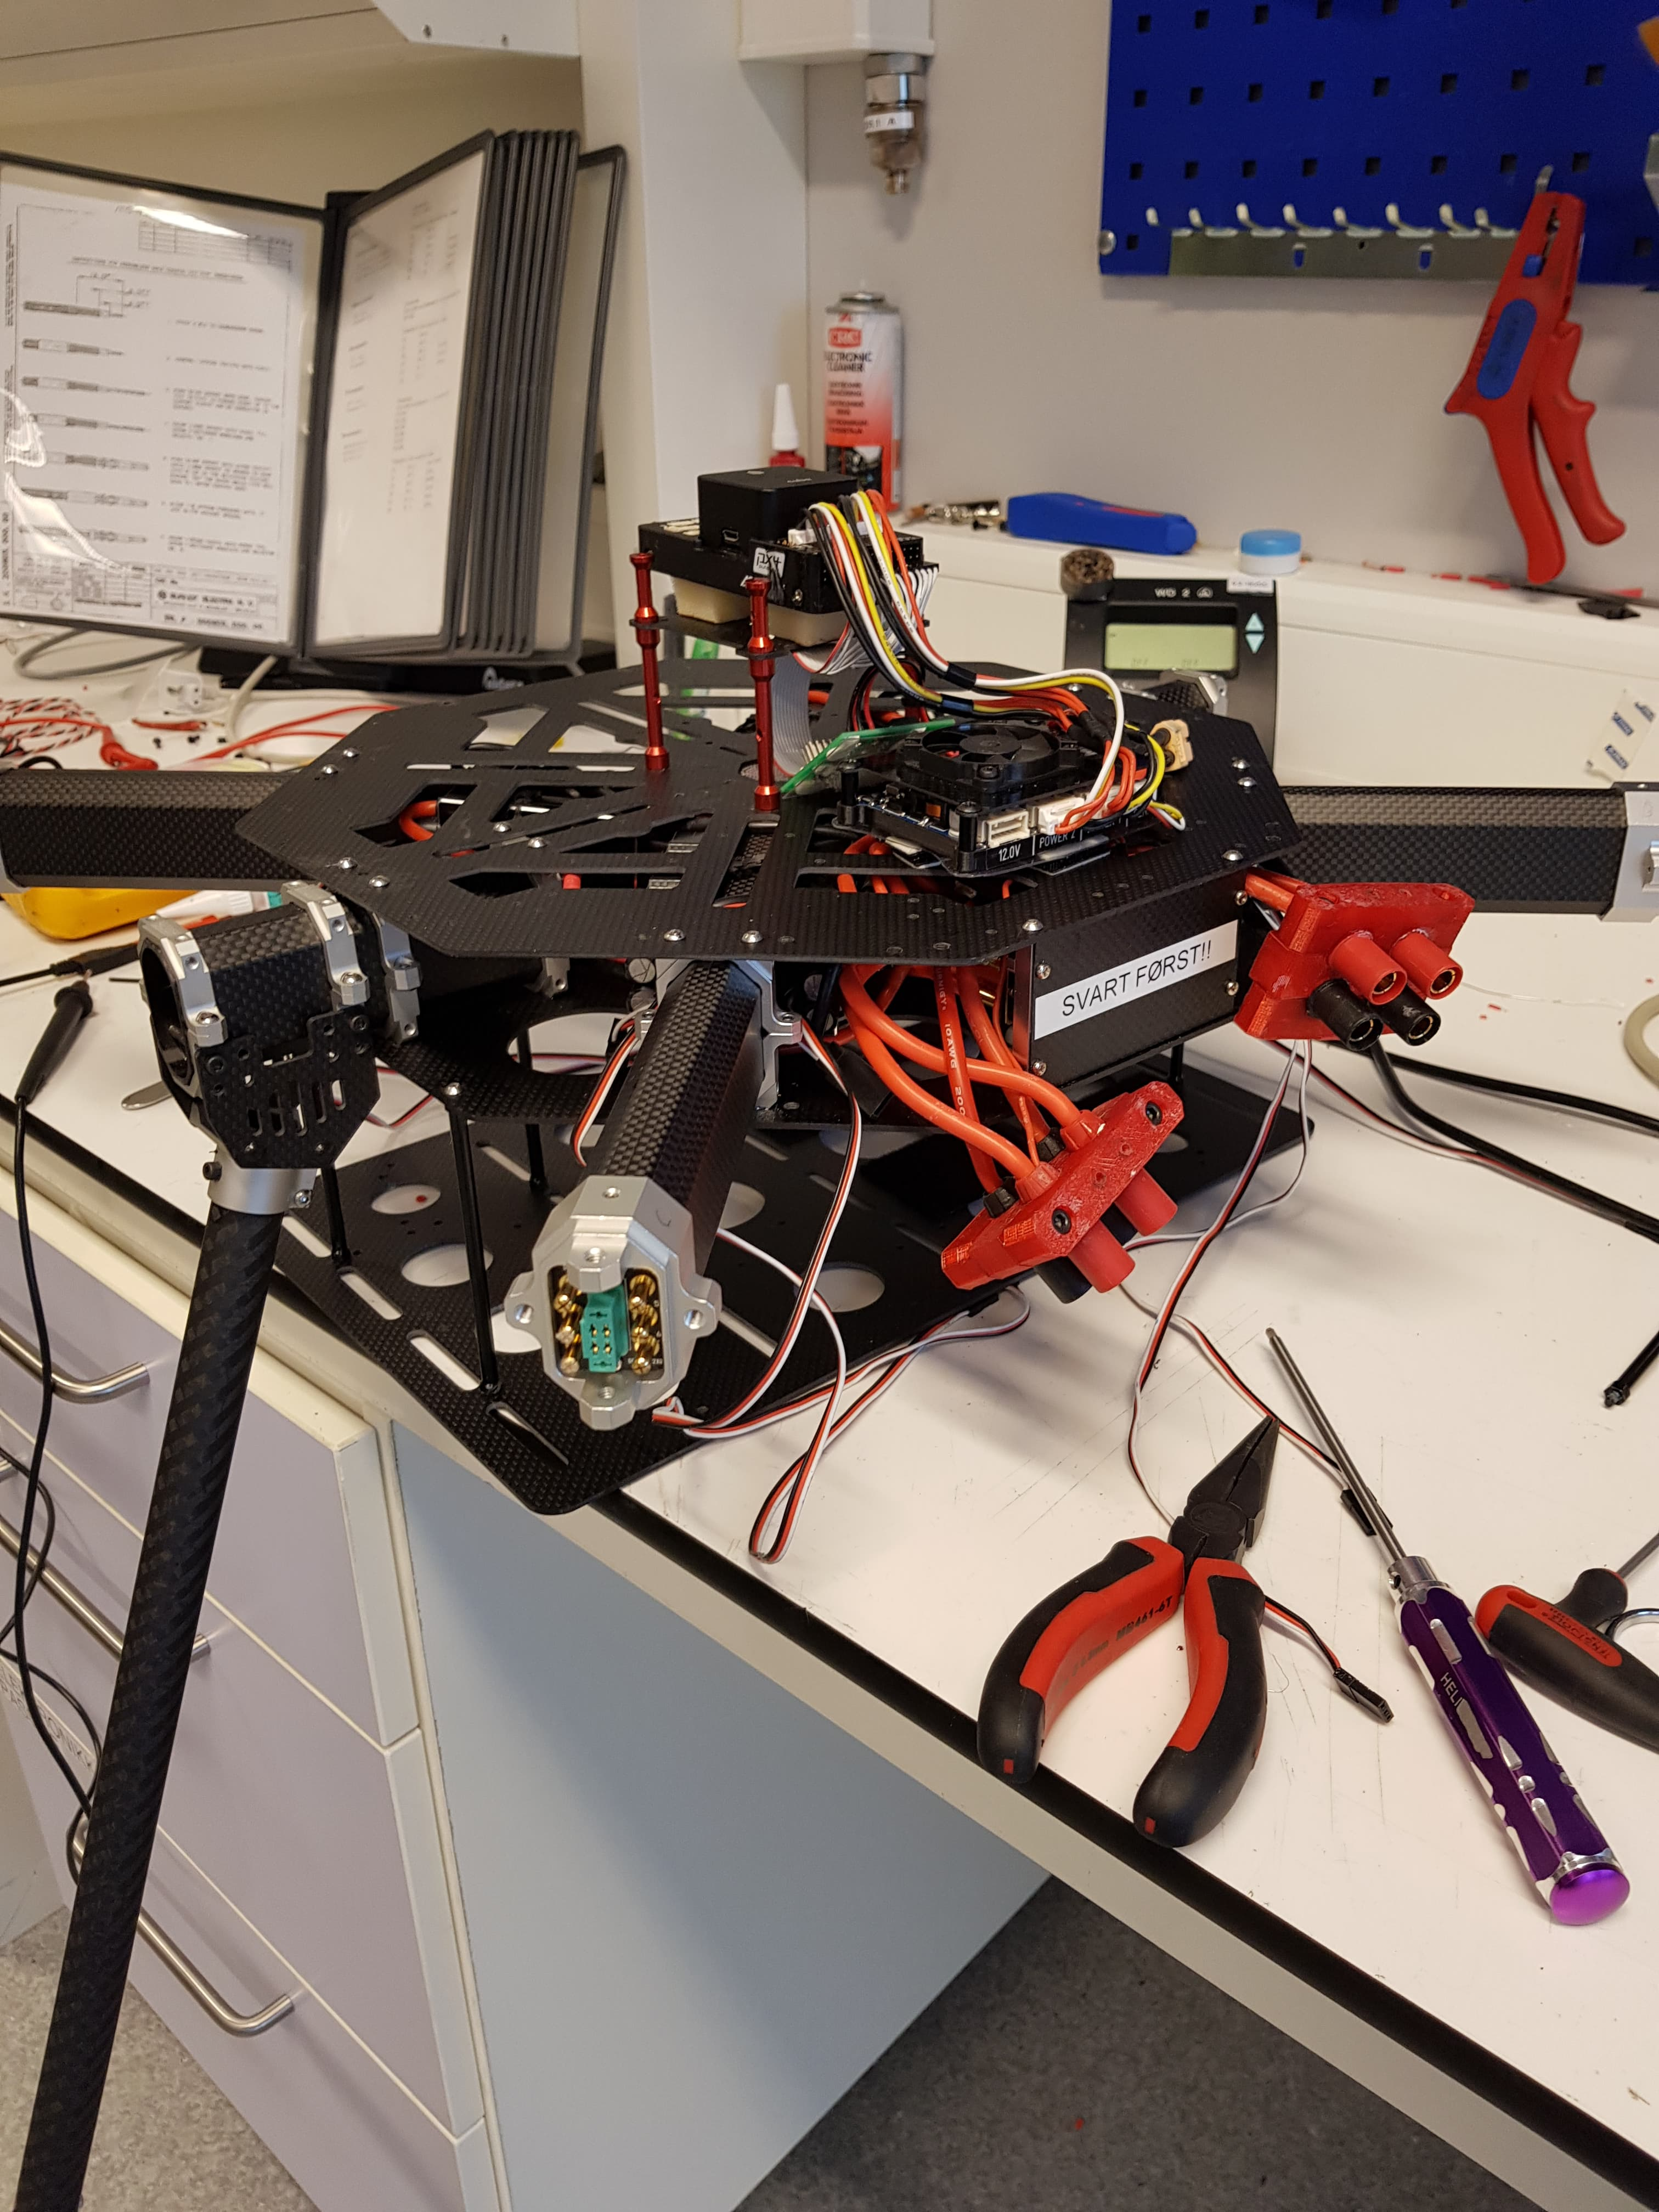
\includegraphics[height = 8cm, width = 0.6\textwidth]{bilder/octocopt_x8.jpg}
	\caption[Reparasjonsarbeid]{Reparasjonsarbeid på en octocopter i såkalt X8 - konfigurasjon.}
\end{figure}
%Teknisk prosjekt - Cryowing Observer
%\newpage
\begin{figure}[ht]
	\centering
	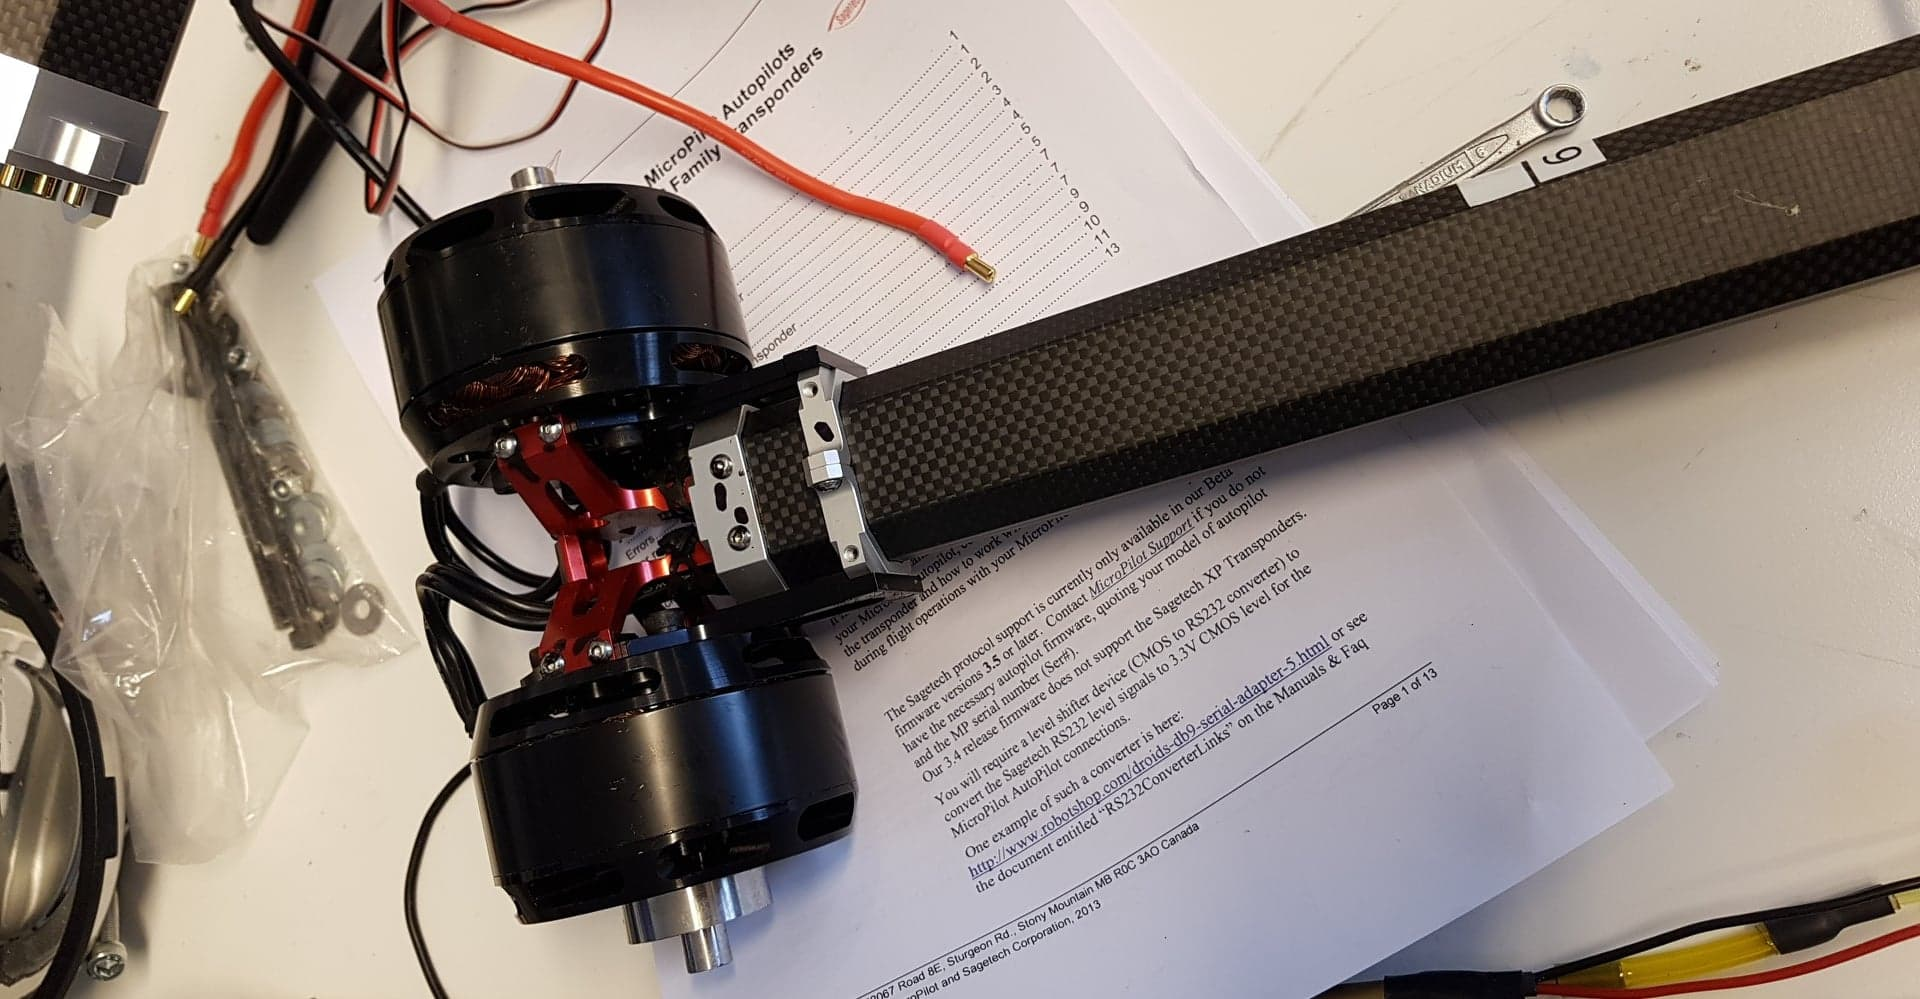
\includegraphics[scale=.2]{bilder/octarm_x8.jpg}
	\caption[Motormontering]{Montering av nye motorer på ytre armer.}
\end{figure}

\subsection{Påfølgende uker: Byggeprosjekt}
\subsubsection{Montering}
Da jeg endelig fikk delene til Cryowing Observer - fartøyene, kunne jeg begynne prosjektet. Hele denne uken og neste uke gikk til bygging av første flykropp. Dette tok lang tid da det var lite med ressurser og folk til hjelp for å kunne få flyet ferdig i løpet av første prosjektuke. Ikke alle delene fra Bodø ble hentet opp, og materialene var dårlig systematisert. Det gikk mye tid i å finne riktige materialer til de ulike delene.\\
Til tross for dette var dette en fin oppgave i å få utforske og prøve ulike metoder for å komme frem til en løsning. Jeg har jobbet med multirotorer før, men montering av servoer og håndtering av EPO-materiale var helt nytt for meg. Det var dermed en bratt læringskurve. \\ Min plan for gjennomføring av byggeprosjektet var å sette sammen flyene med servoer, kropp, vinger og utstyrskuppel, se bildene under.
%Vis bilde av byggingen 

Jeg begynte med montering av vingene, ved å sette på servoer og lime kryssfiner-sparrer til vingene. Servoene ble festet med enten varmlim eller lynlim. Alle servoene som settes på måtte sentreres ved hjelp av en servo-tester, slik at det blir enklest å sette opp flyet elektronisk. 

\begin{figure}[ht]
	\centering
	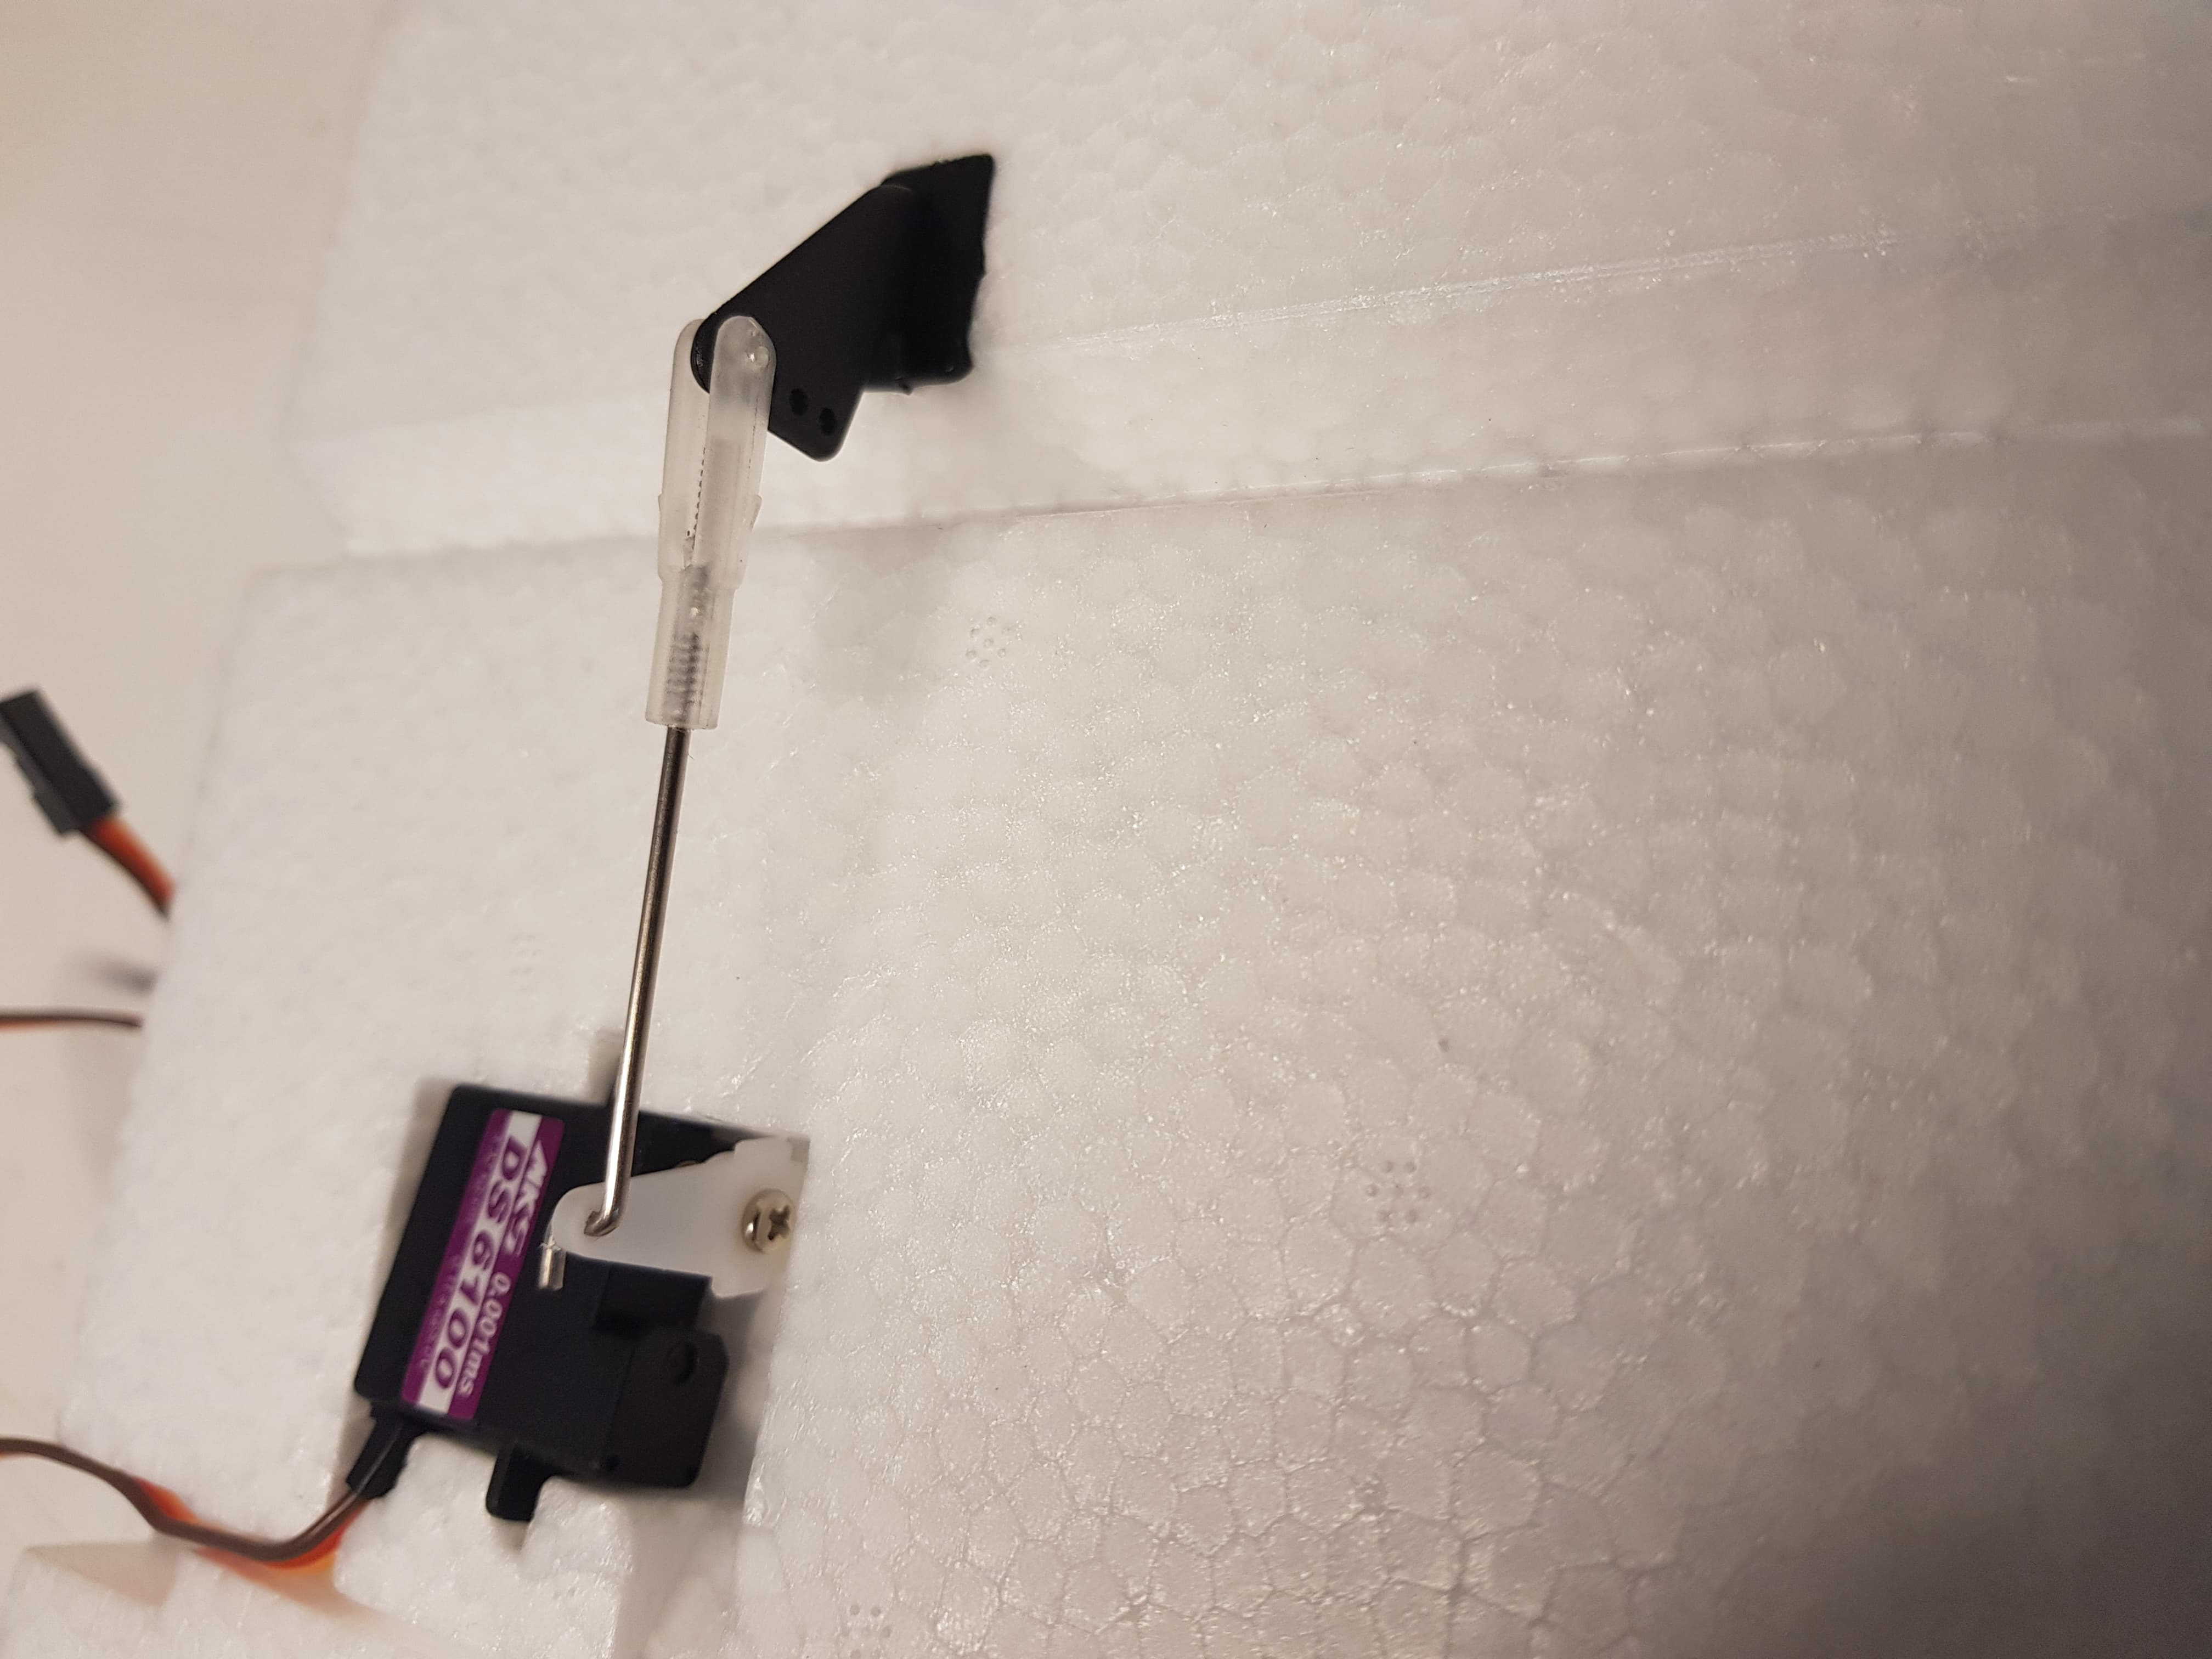
\includegraphics[height = 10cm, width = .6\textwidth]{bilder/servomontering.jpg}
	\caption[Servoorientering]{Riktig montering av servo, der servohornet er \ang{90} med horisontalplanet (her vingen).}
\end{figure}



\begin{figure}[ht]
	\centering
	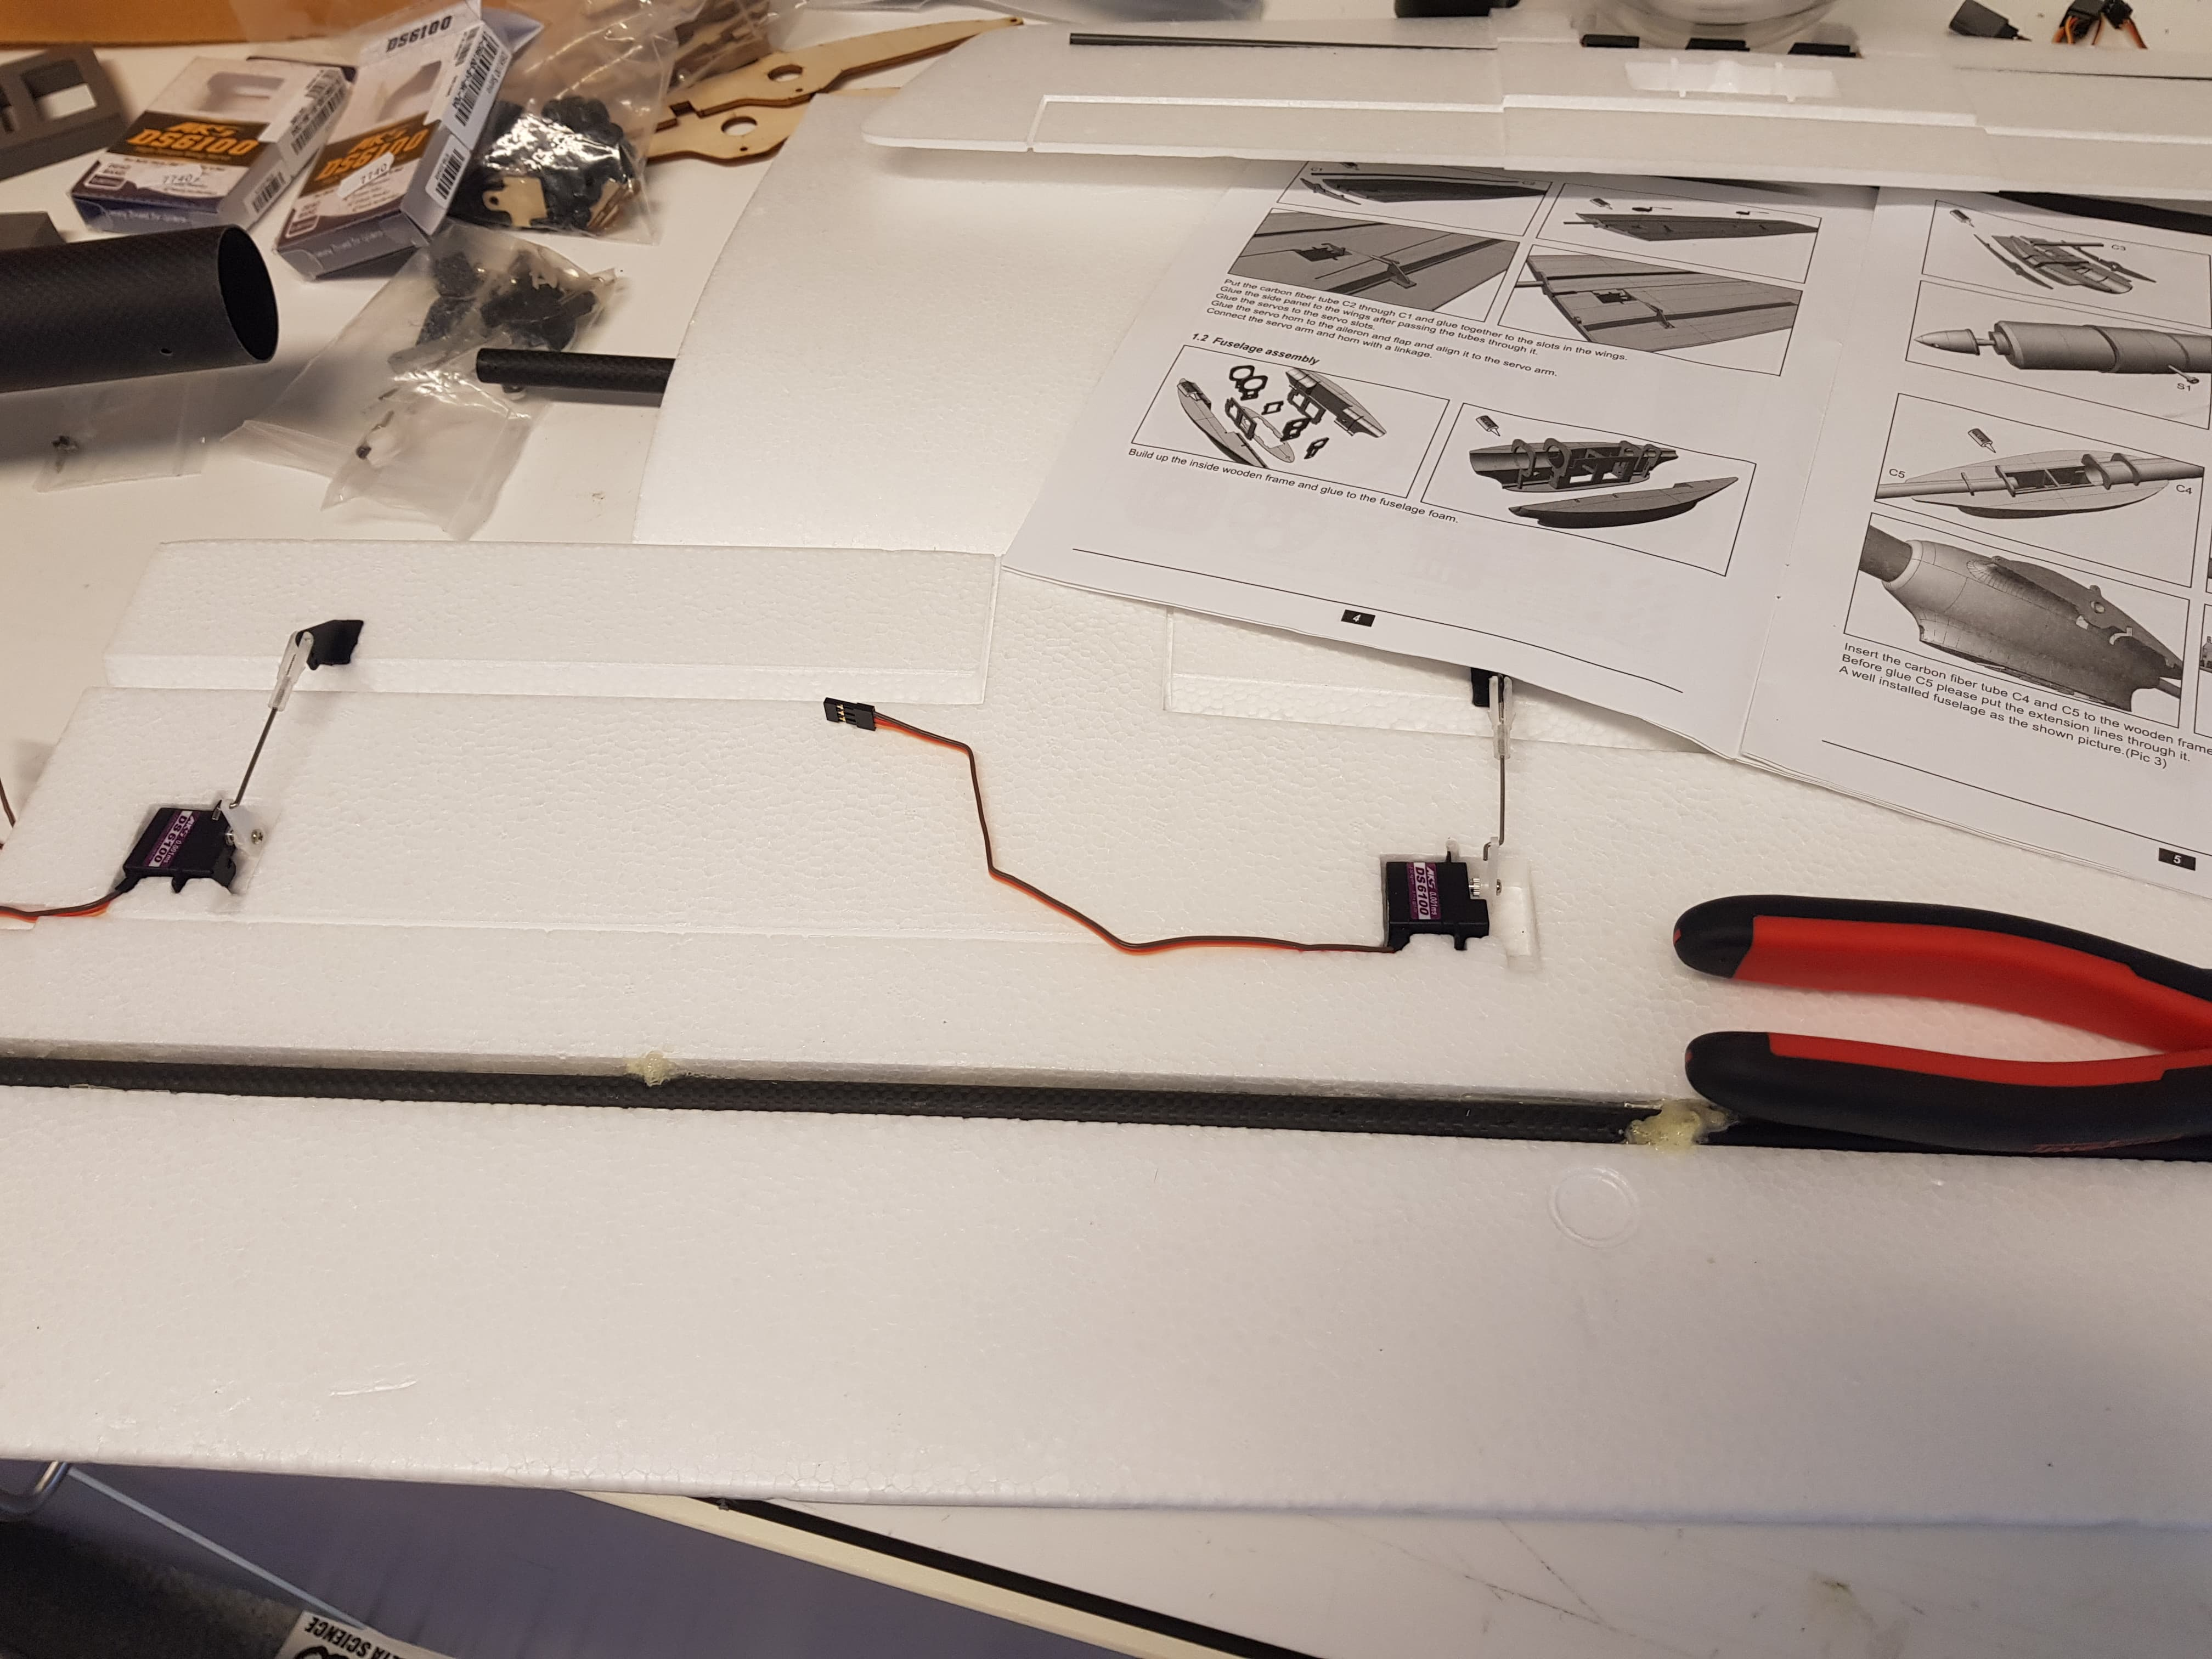
\includegraphics[width=.6\textwidth,  height = 8cm]{bilder/vingemontering.jpg}
	\caption{Montering av vinger}
\end{figure}

\newpage
Deretter gikk det til montering av motor på det fremre karbonbommen. Motoren, som er av typen BLDC (børsteløs DC-motor), drives av en fartsregulator, populært kalt ESC. Denne ESC'en inneholder en spenningsregulator som tar inn batterispenningen og gir ut en konstant 5V-kilde som kan brukes til å forsyne mottaker og annet periferier med spenning. 

\begin{figure}[ht]
	\centering
	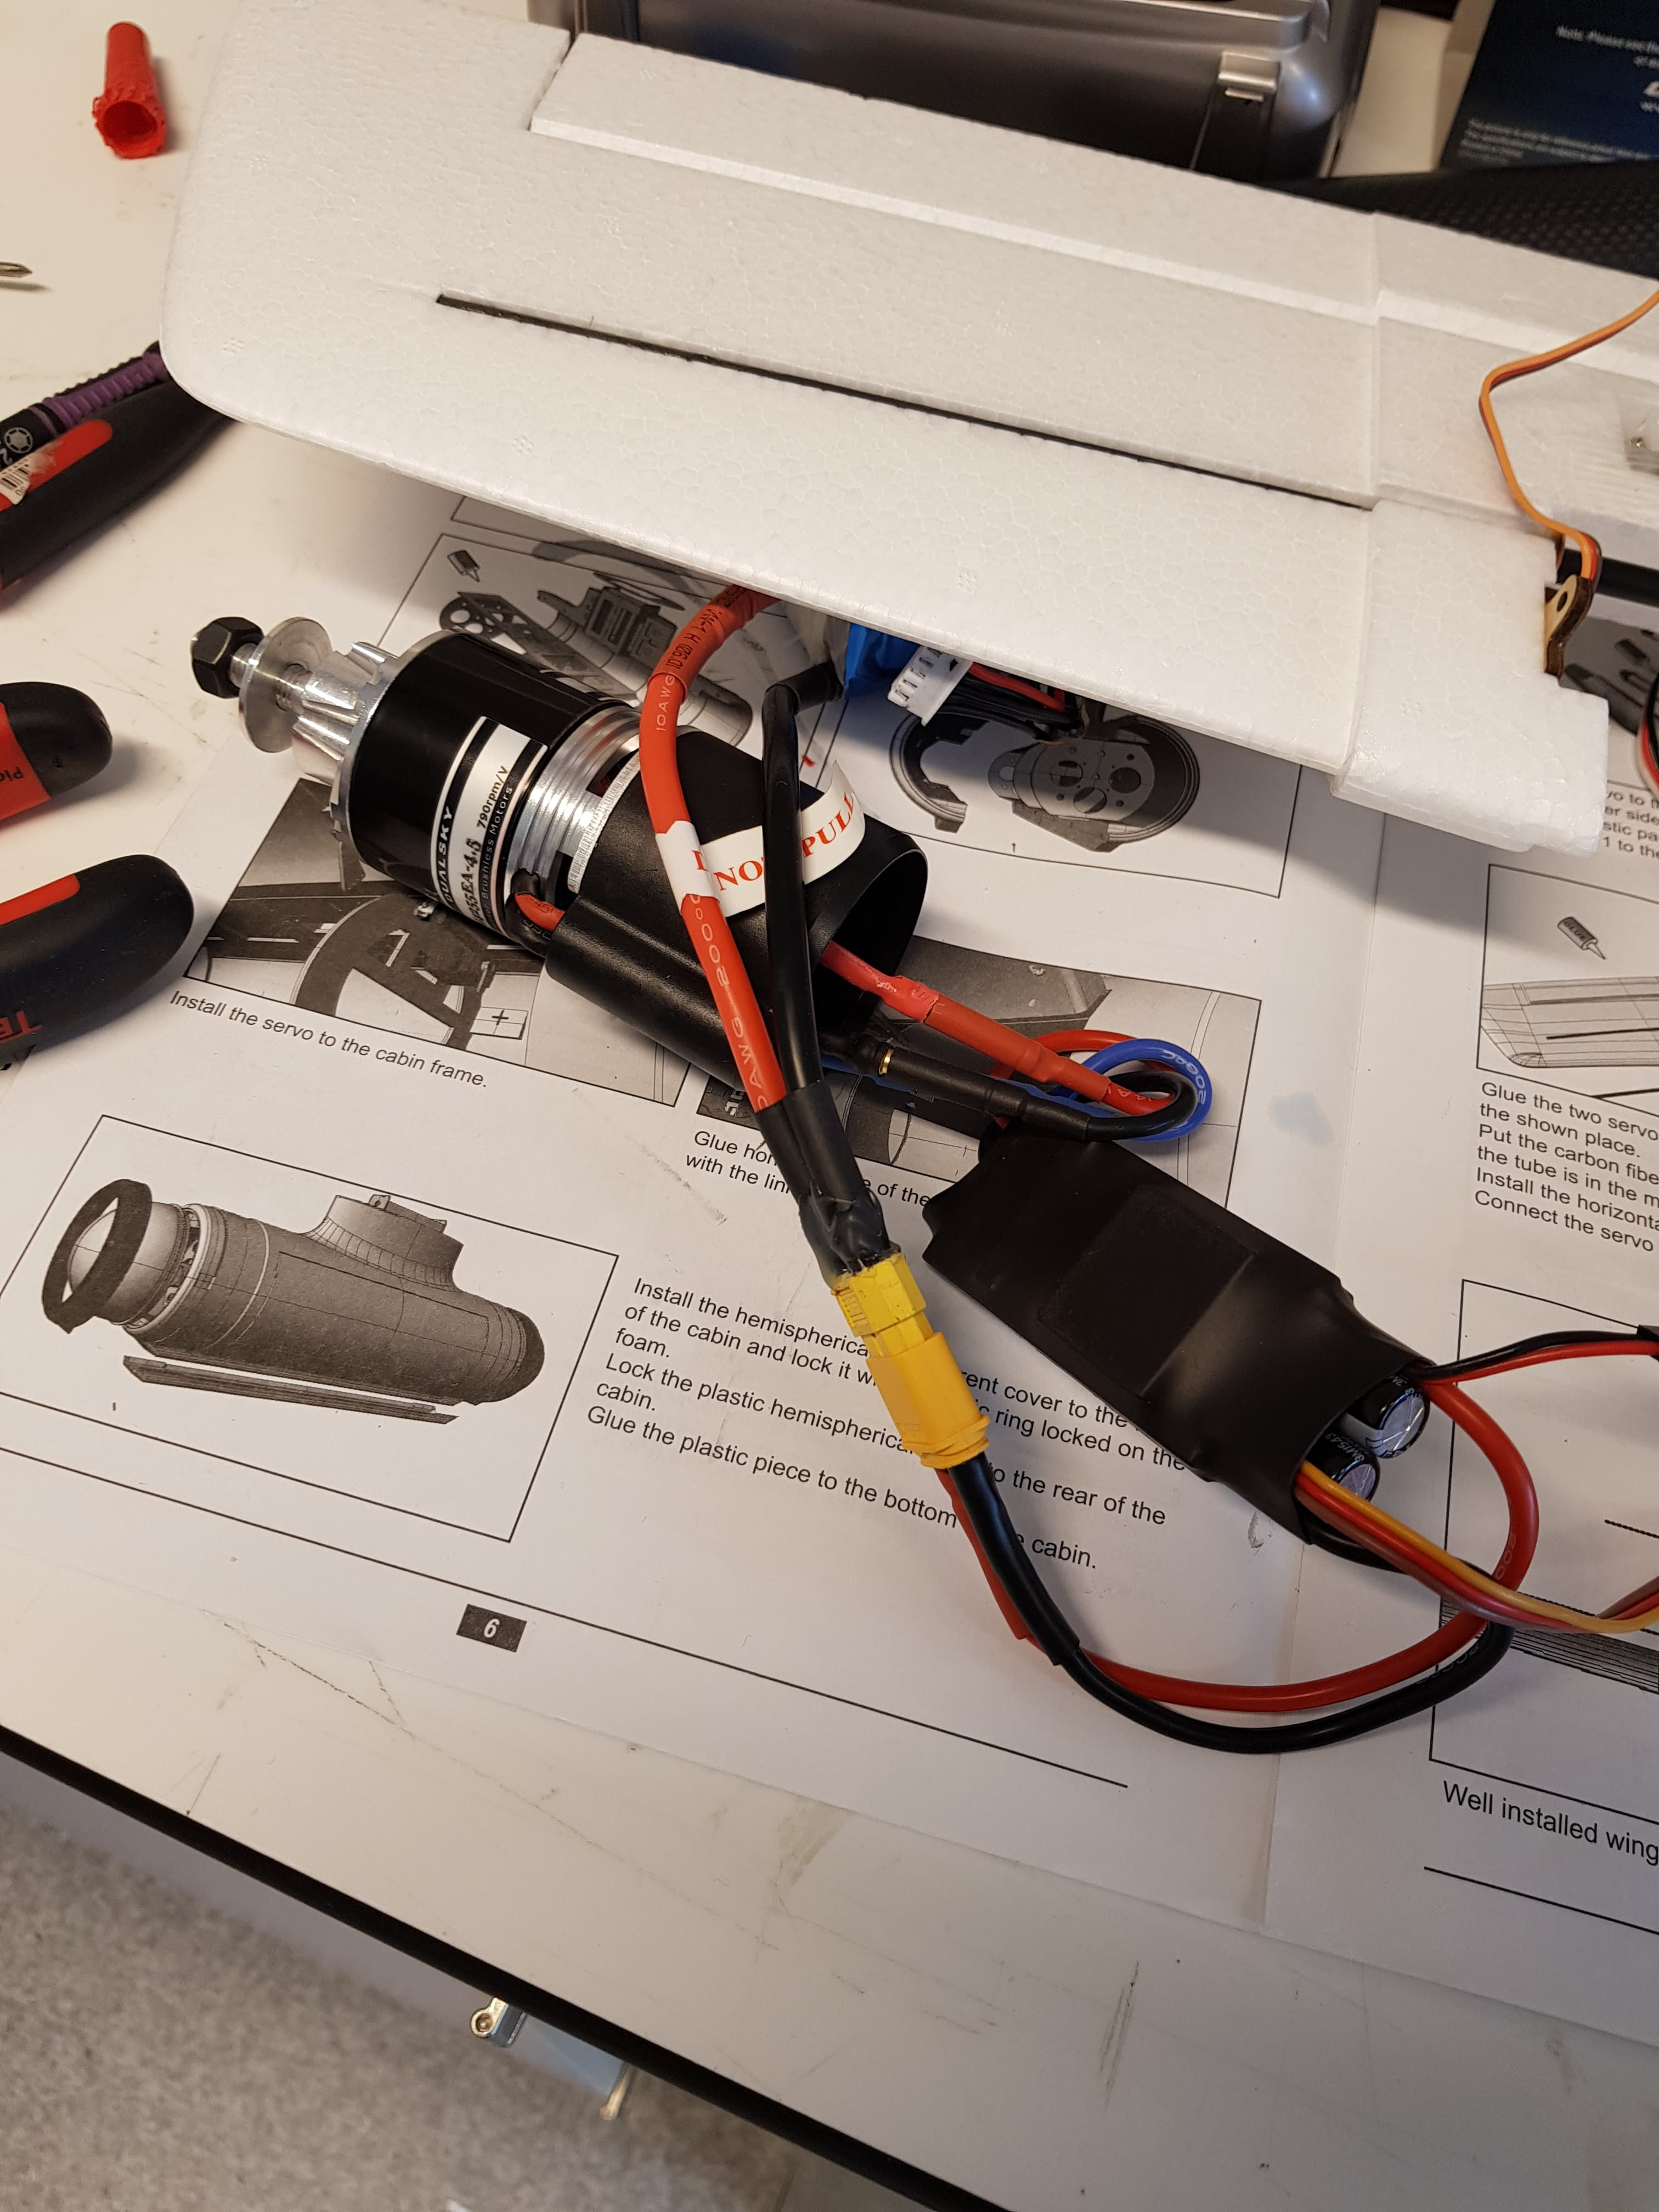
\includegraphics[height=7.6cm, width = .55\textwidth]{bilder/esc_og_motor.jpg}
	\caption[Observer-motor]{Motor tilkoblet ESC, med bryter bypassed. XT-60 - connectoren (den gule pluggen) måtte loddes på ESC-enden.}
\end{figure}

\newpage
Etter påmontert motor på karbonrøret, kunne røret limes på til undersiden av den midtre flykroppen ved hjelp av epoxy. Men på grunn av at epoxy ikke skaper en god kjemisk binding med EPO/isopor, men bare en fysisk binding, måtte jeg gjøre overflaten så stor som mulig. Jeg pusset begge overflatene med grovt sandpapir og lagde flere hull i EPO'en slik at epoxyen kan feste seg. 
Men ting gikk ikke helt som planlagt, da jeg fikk vite underveis at visse deler hadde jeg montert feil, slik som at et karbonrør var for langt inn i kroppen. Da blokkerer det bakre karbonrøret for eventuell GPS som kan monteres inni ramma. Dette førte til at jeg måtte hule ut overkroppen for at den skulle passe til underkroppen. \\
Dessuten hadde jeg aldri brukt epoxy før og visste ikke hvordan man skulle få godt nok feste mellom materialene. Første forsøk på liming ble derfor dårlig og måtte gjøres på nytt. Jeg fikk ingen veiledning på dette, bare at dette måtte gjøres om igjen. Til slutt, etter to forsøk, fikk jeg hjelp av en til å få godt nok feste. Epoxyen måtte tilsettes fyllmiddel for å kompansere for all materiale som ble skrapet av. \\


\begin{figure}[ht]
	\centering
	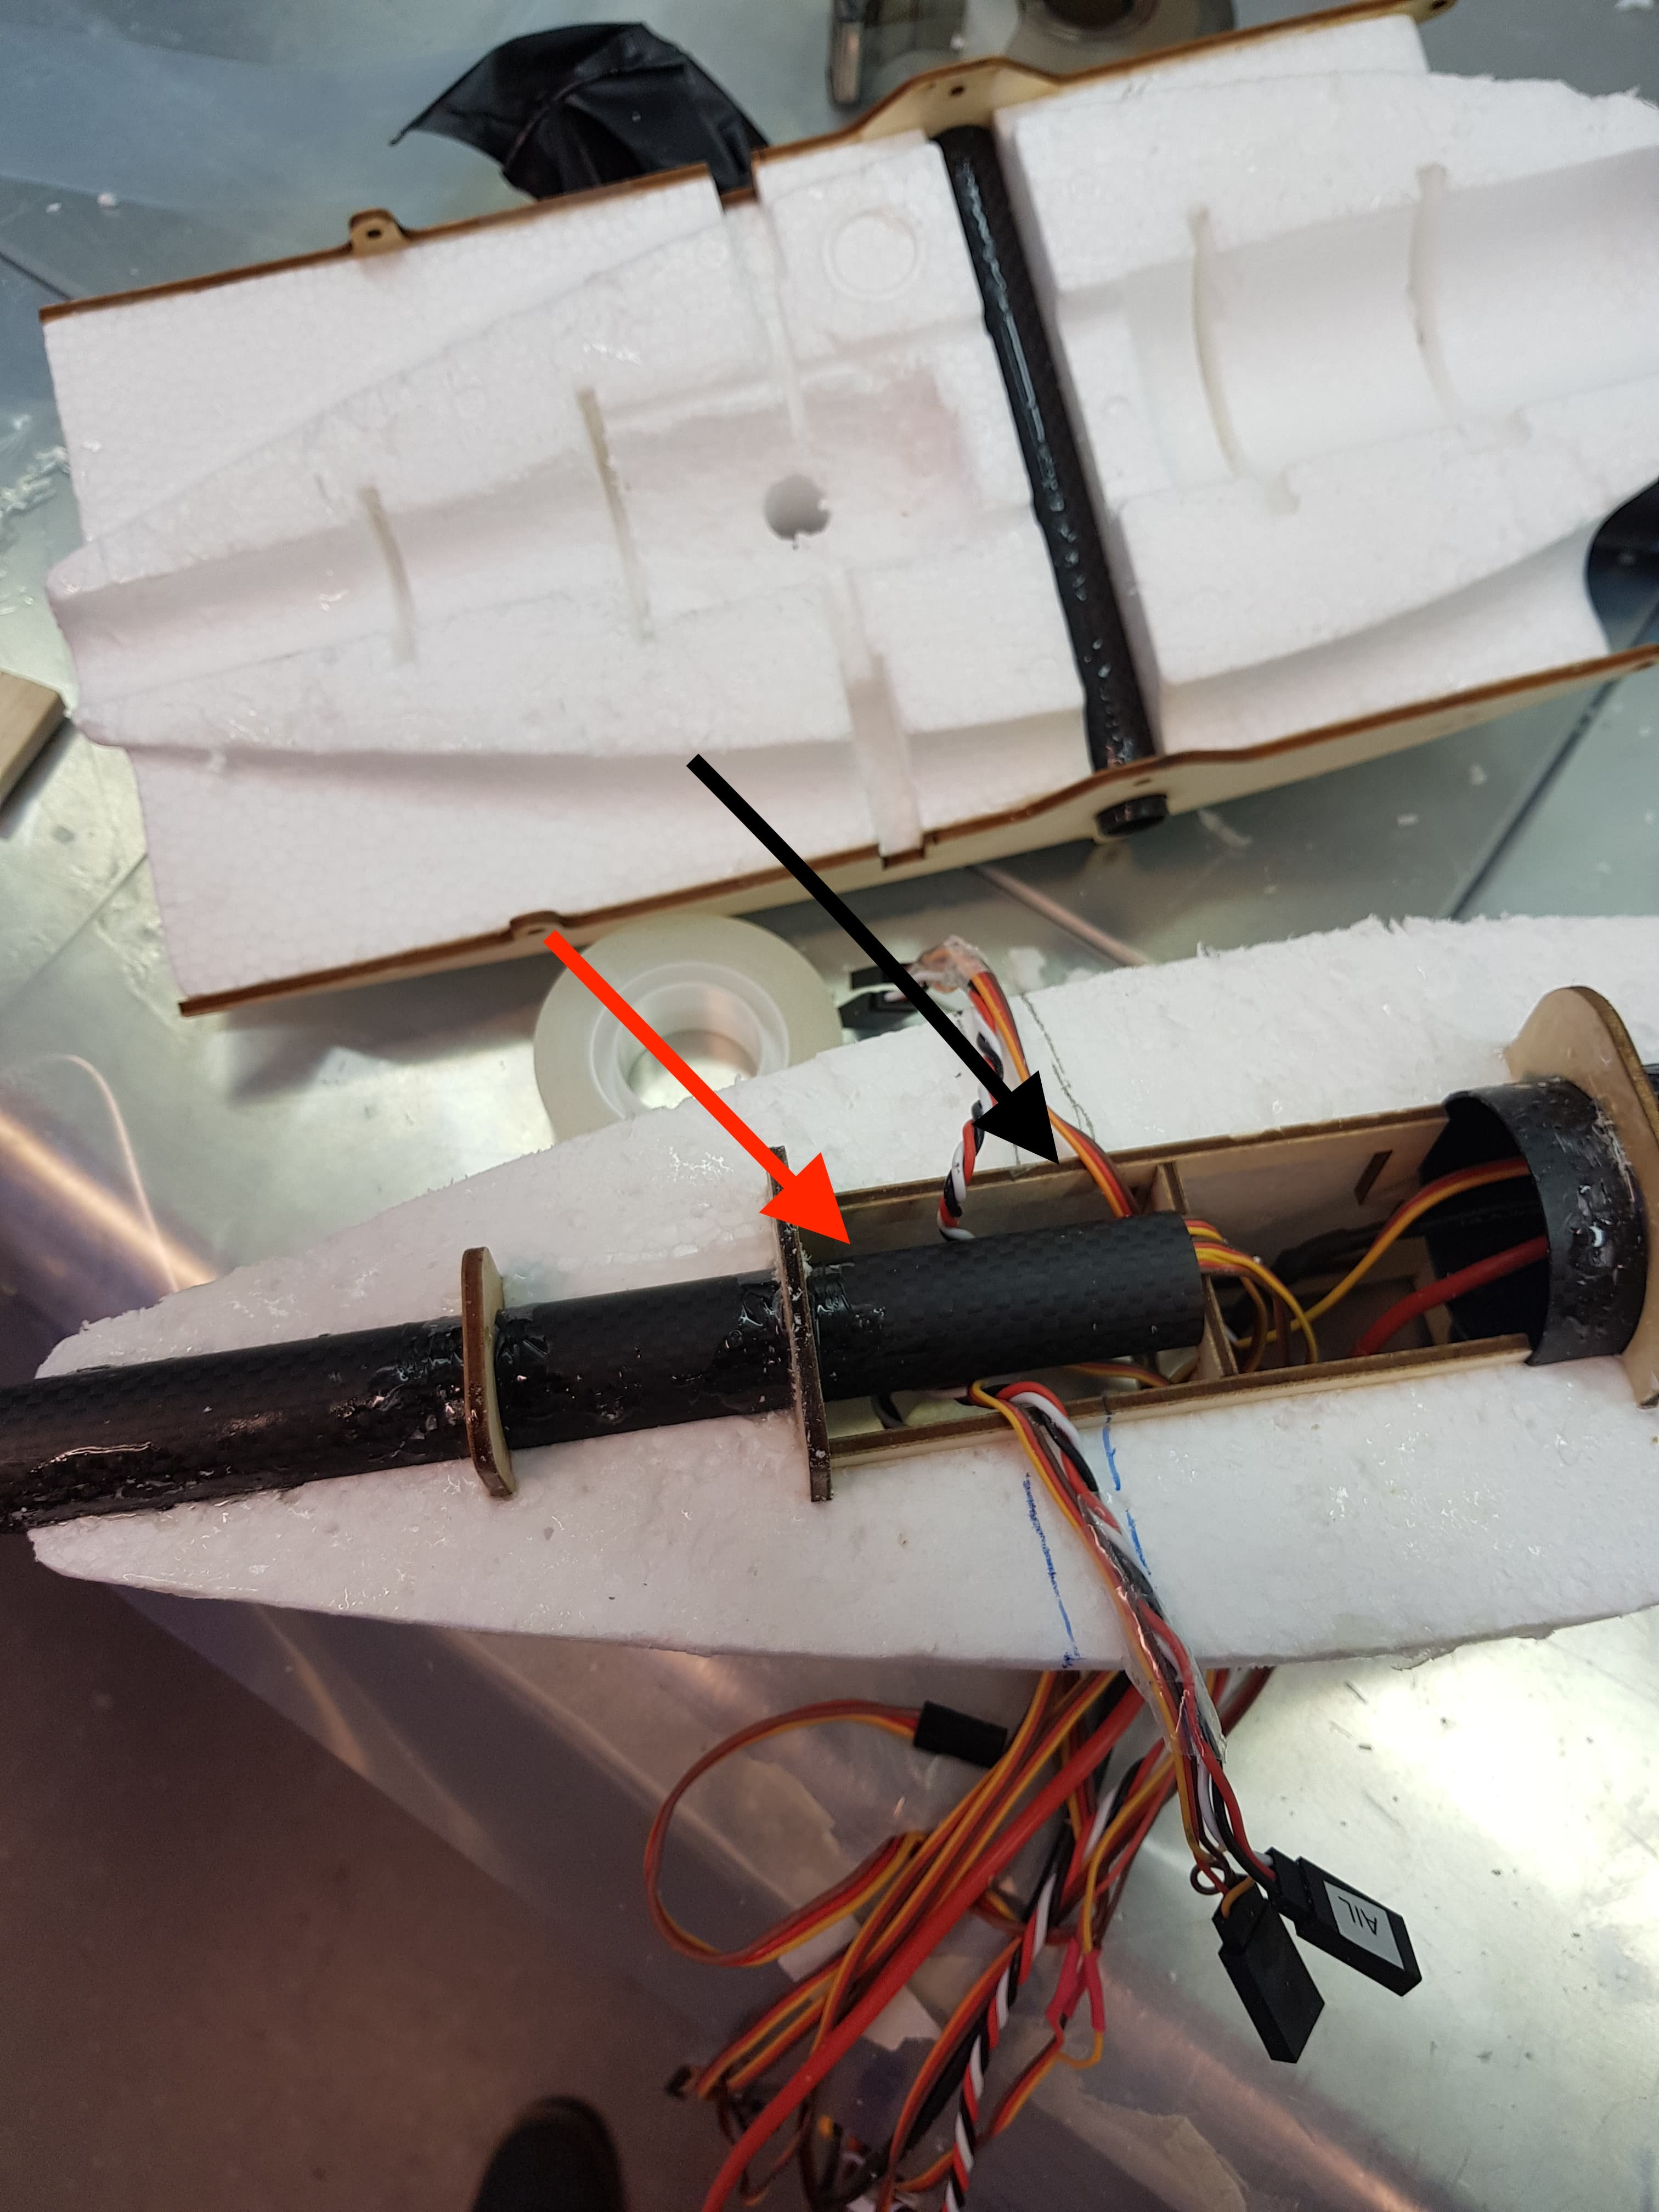
\includegraphics[height = 7cm, width = .6\textwidth]{bilder/feilmontering_av_karbon_red.jpg}
	\caption[Feilliming]{Det bakre karbonrøret ble limt for langt frem, og blokkerte for eventuell GPS-installasjon og påmontering av øvre ramme. Karbonrøret skal egentlig være ved den røde pilen.}
\end{figure}

\begin{figure}[ht]
 \centering
 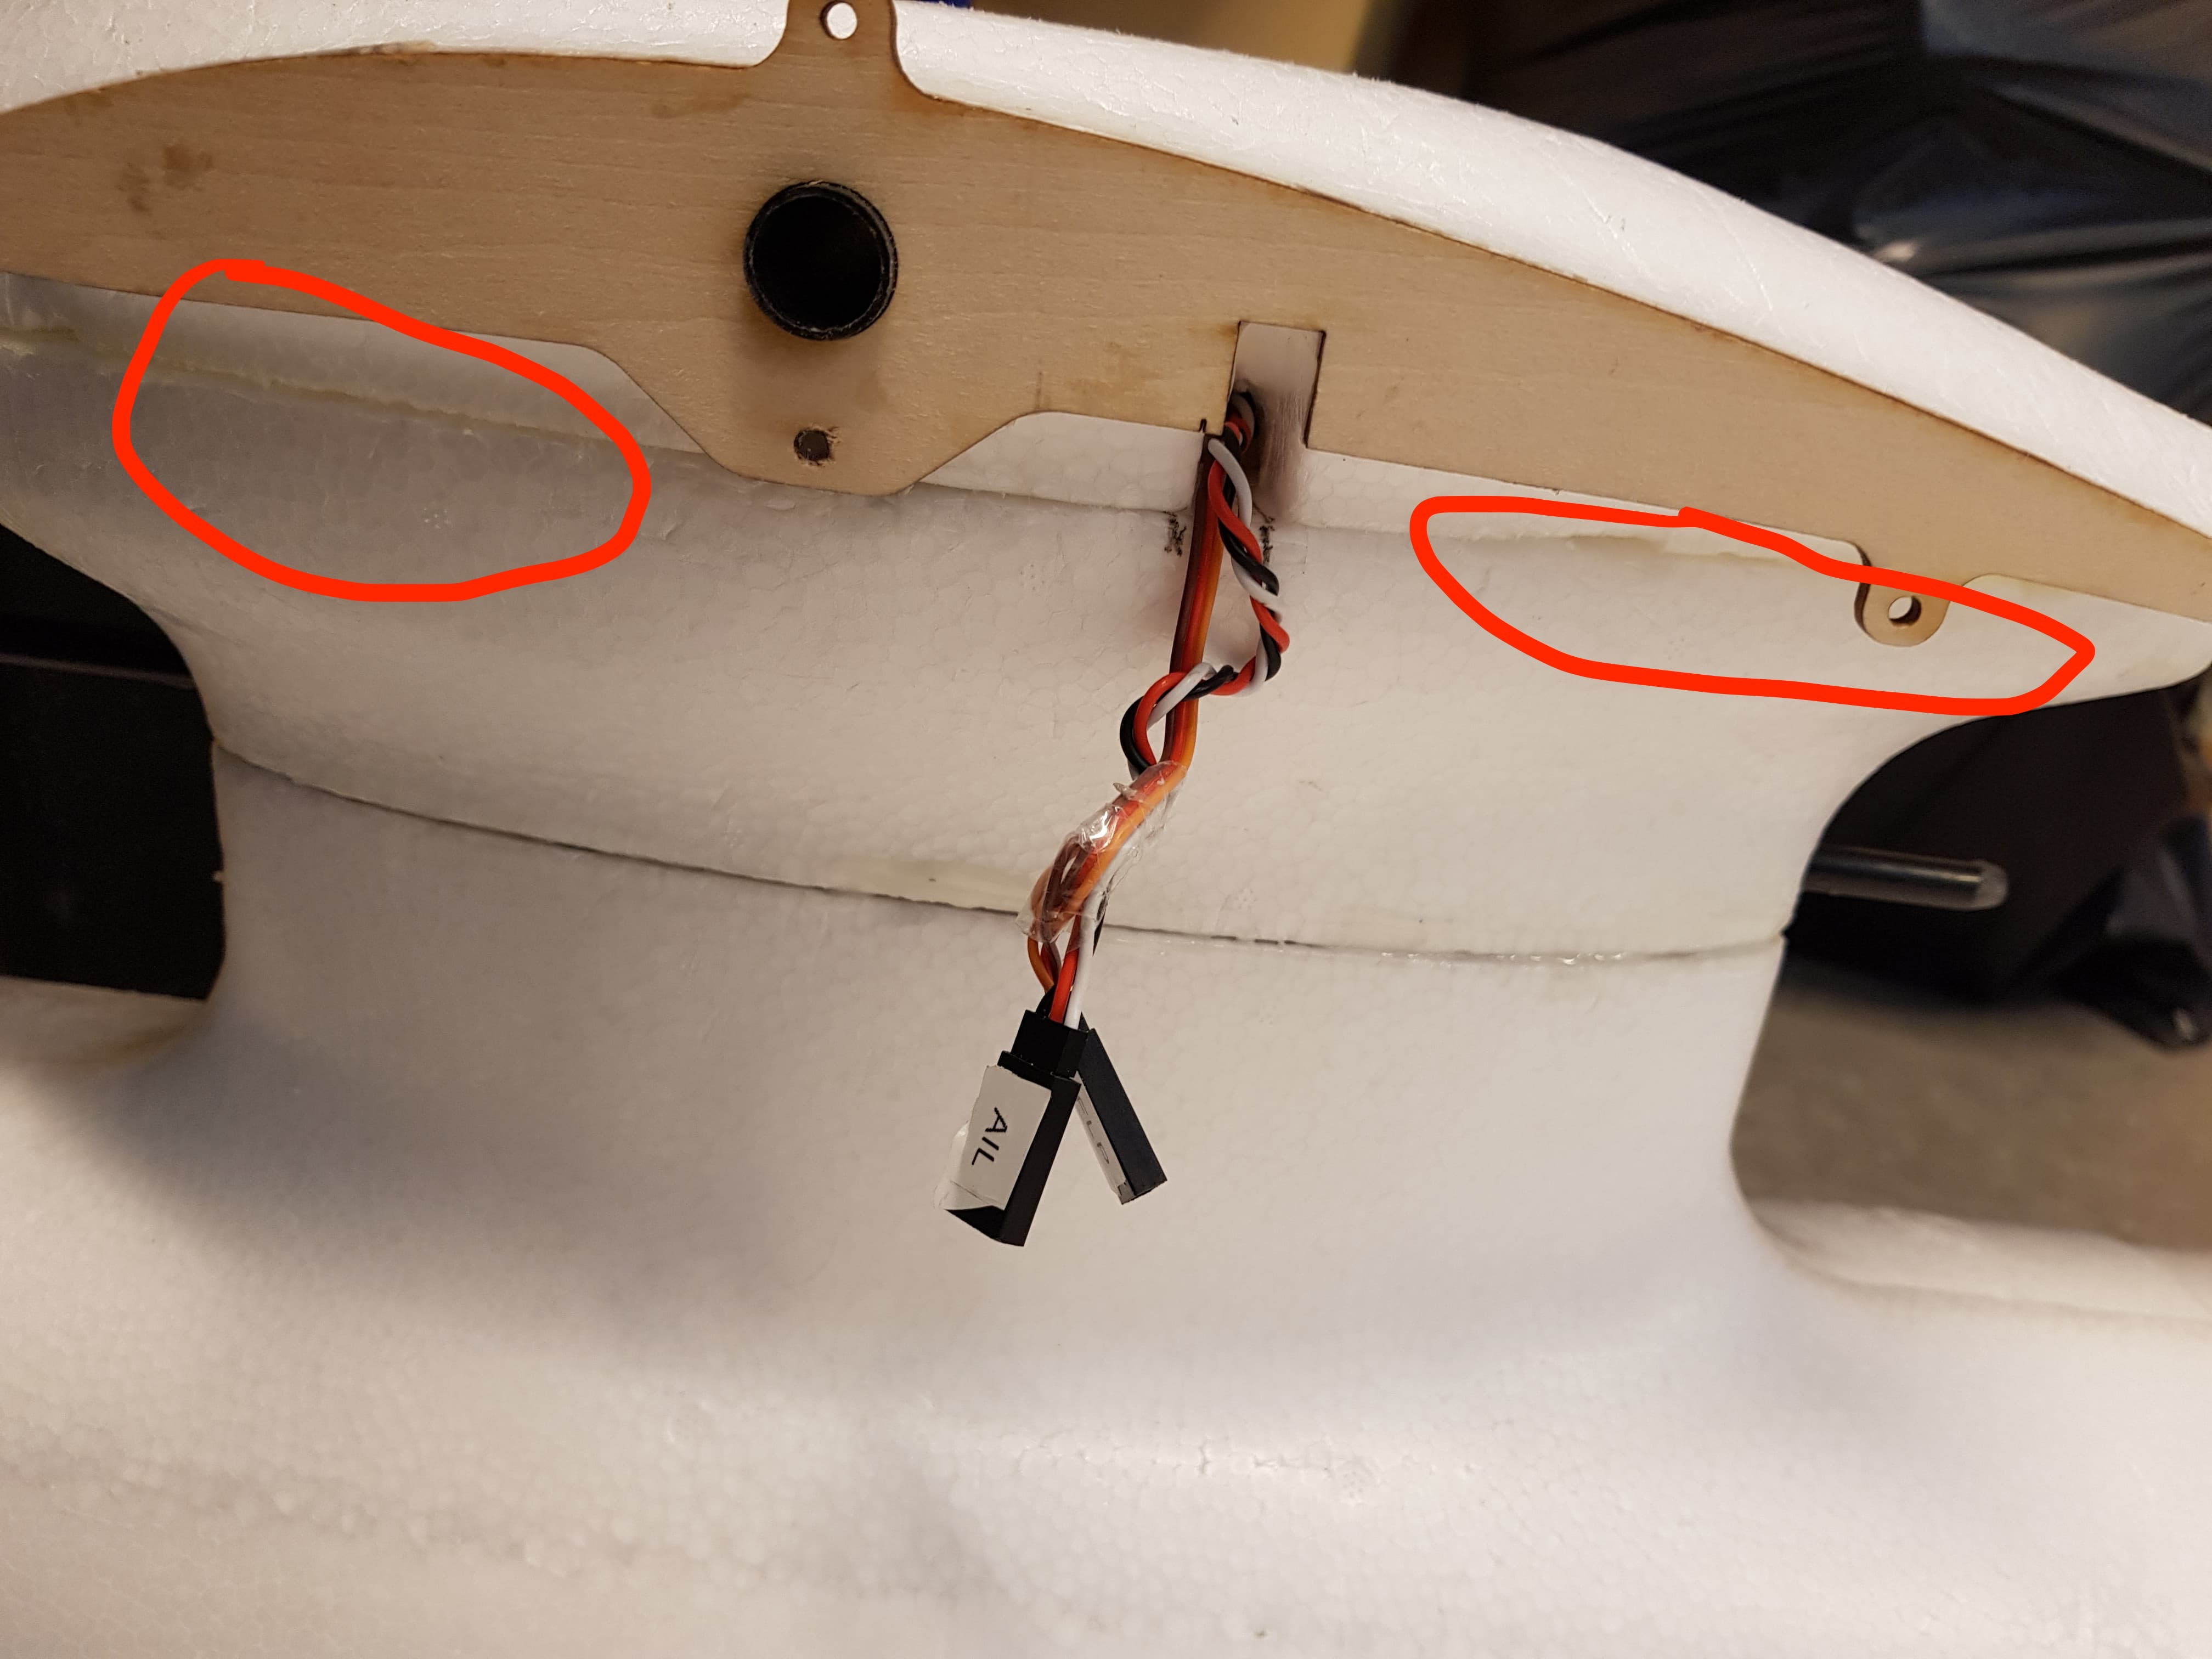
\includegraphics[height=7cm, width = .6\textwidth]{bilder/fylling2_red.jpg}
 \caption[Endelig limeresultat]{Endeling resultat av limingen. Merk det fylte området.}
\end{figure}
\newpage

Mens dette sto og herdet, fortsatte jeg arbeidet ved å montere halen. Jeg glemte å ta bilder av denne monteringen. Etter halen gjenstod monteringen av utstyrskammeret. Dette kammeret festes med flykroppen ved hjelp av et karbonrør gjennom begge delene, men Norut foretrekker at de er limt sammen med epoxy i tillegg til karbonrørets funksjon. Deretter ble det bare å montere på vingene, koble halen fast, og flyet var klart for første inspeksjon

\begin{figure}[ht]
	\centering
	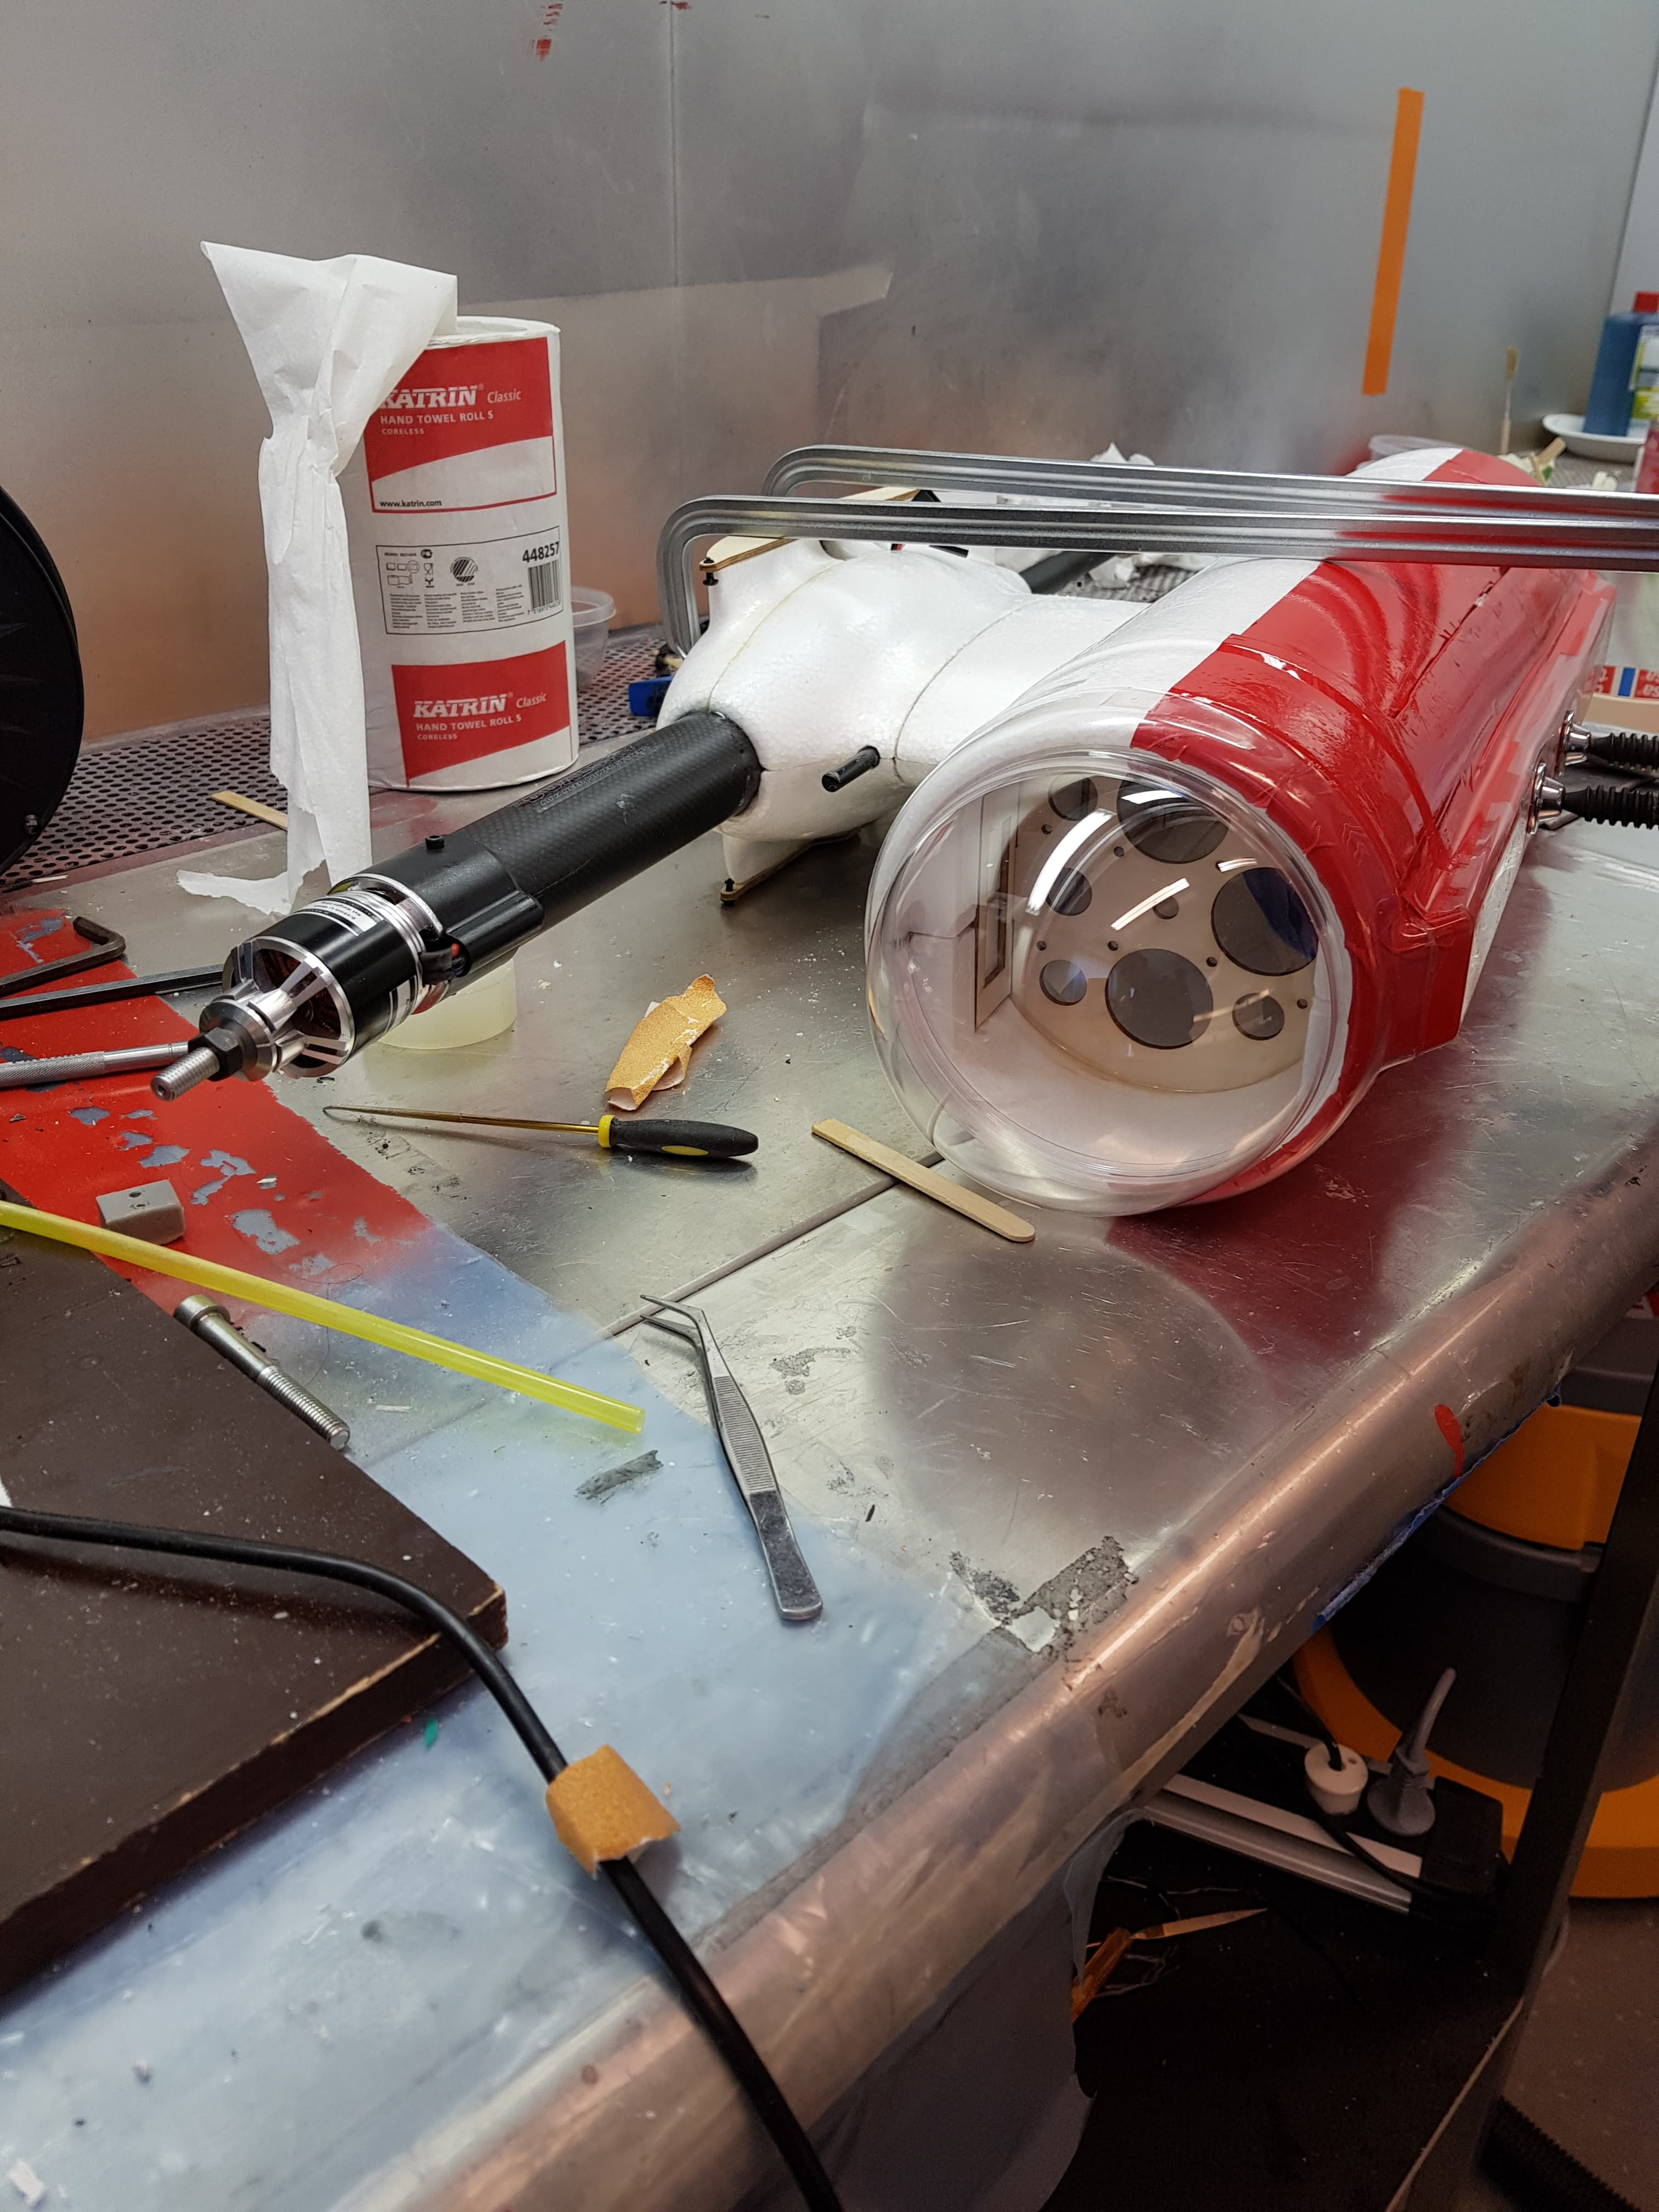
\includegraphics[width = .5\textwidth, height = 8.1cm]{bilder/kammermontering.jpg}
	\caption[Herding av epoxy]{For å holde delene sammen under herding, brukes klemmer for å presse hardt ned. Her ble det brukt 30-minutters epoxy. Det er likevel lurt å la den ligge ''ut dagen'' for best mulig feste.}
\end{figure}
\newpage
\subsubsection{Inspeksjon}
For at et luftfartøy hos Norut skal kunne flys, må det godkjennes og erklæres luftdyktig av teknisk personell. Det første flyet ble ikke godkjent, da halens horisontale stabilisator ikke var i vater. Etter en rask borring av nytt hull i karbonbommen som holder halen fast til selve flykroppen, ble flyet godkjent. Nå kunne elektronikken legges inn. \\

\begin{figure}[ht]
	\centering
	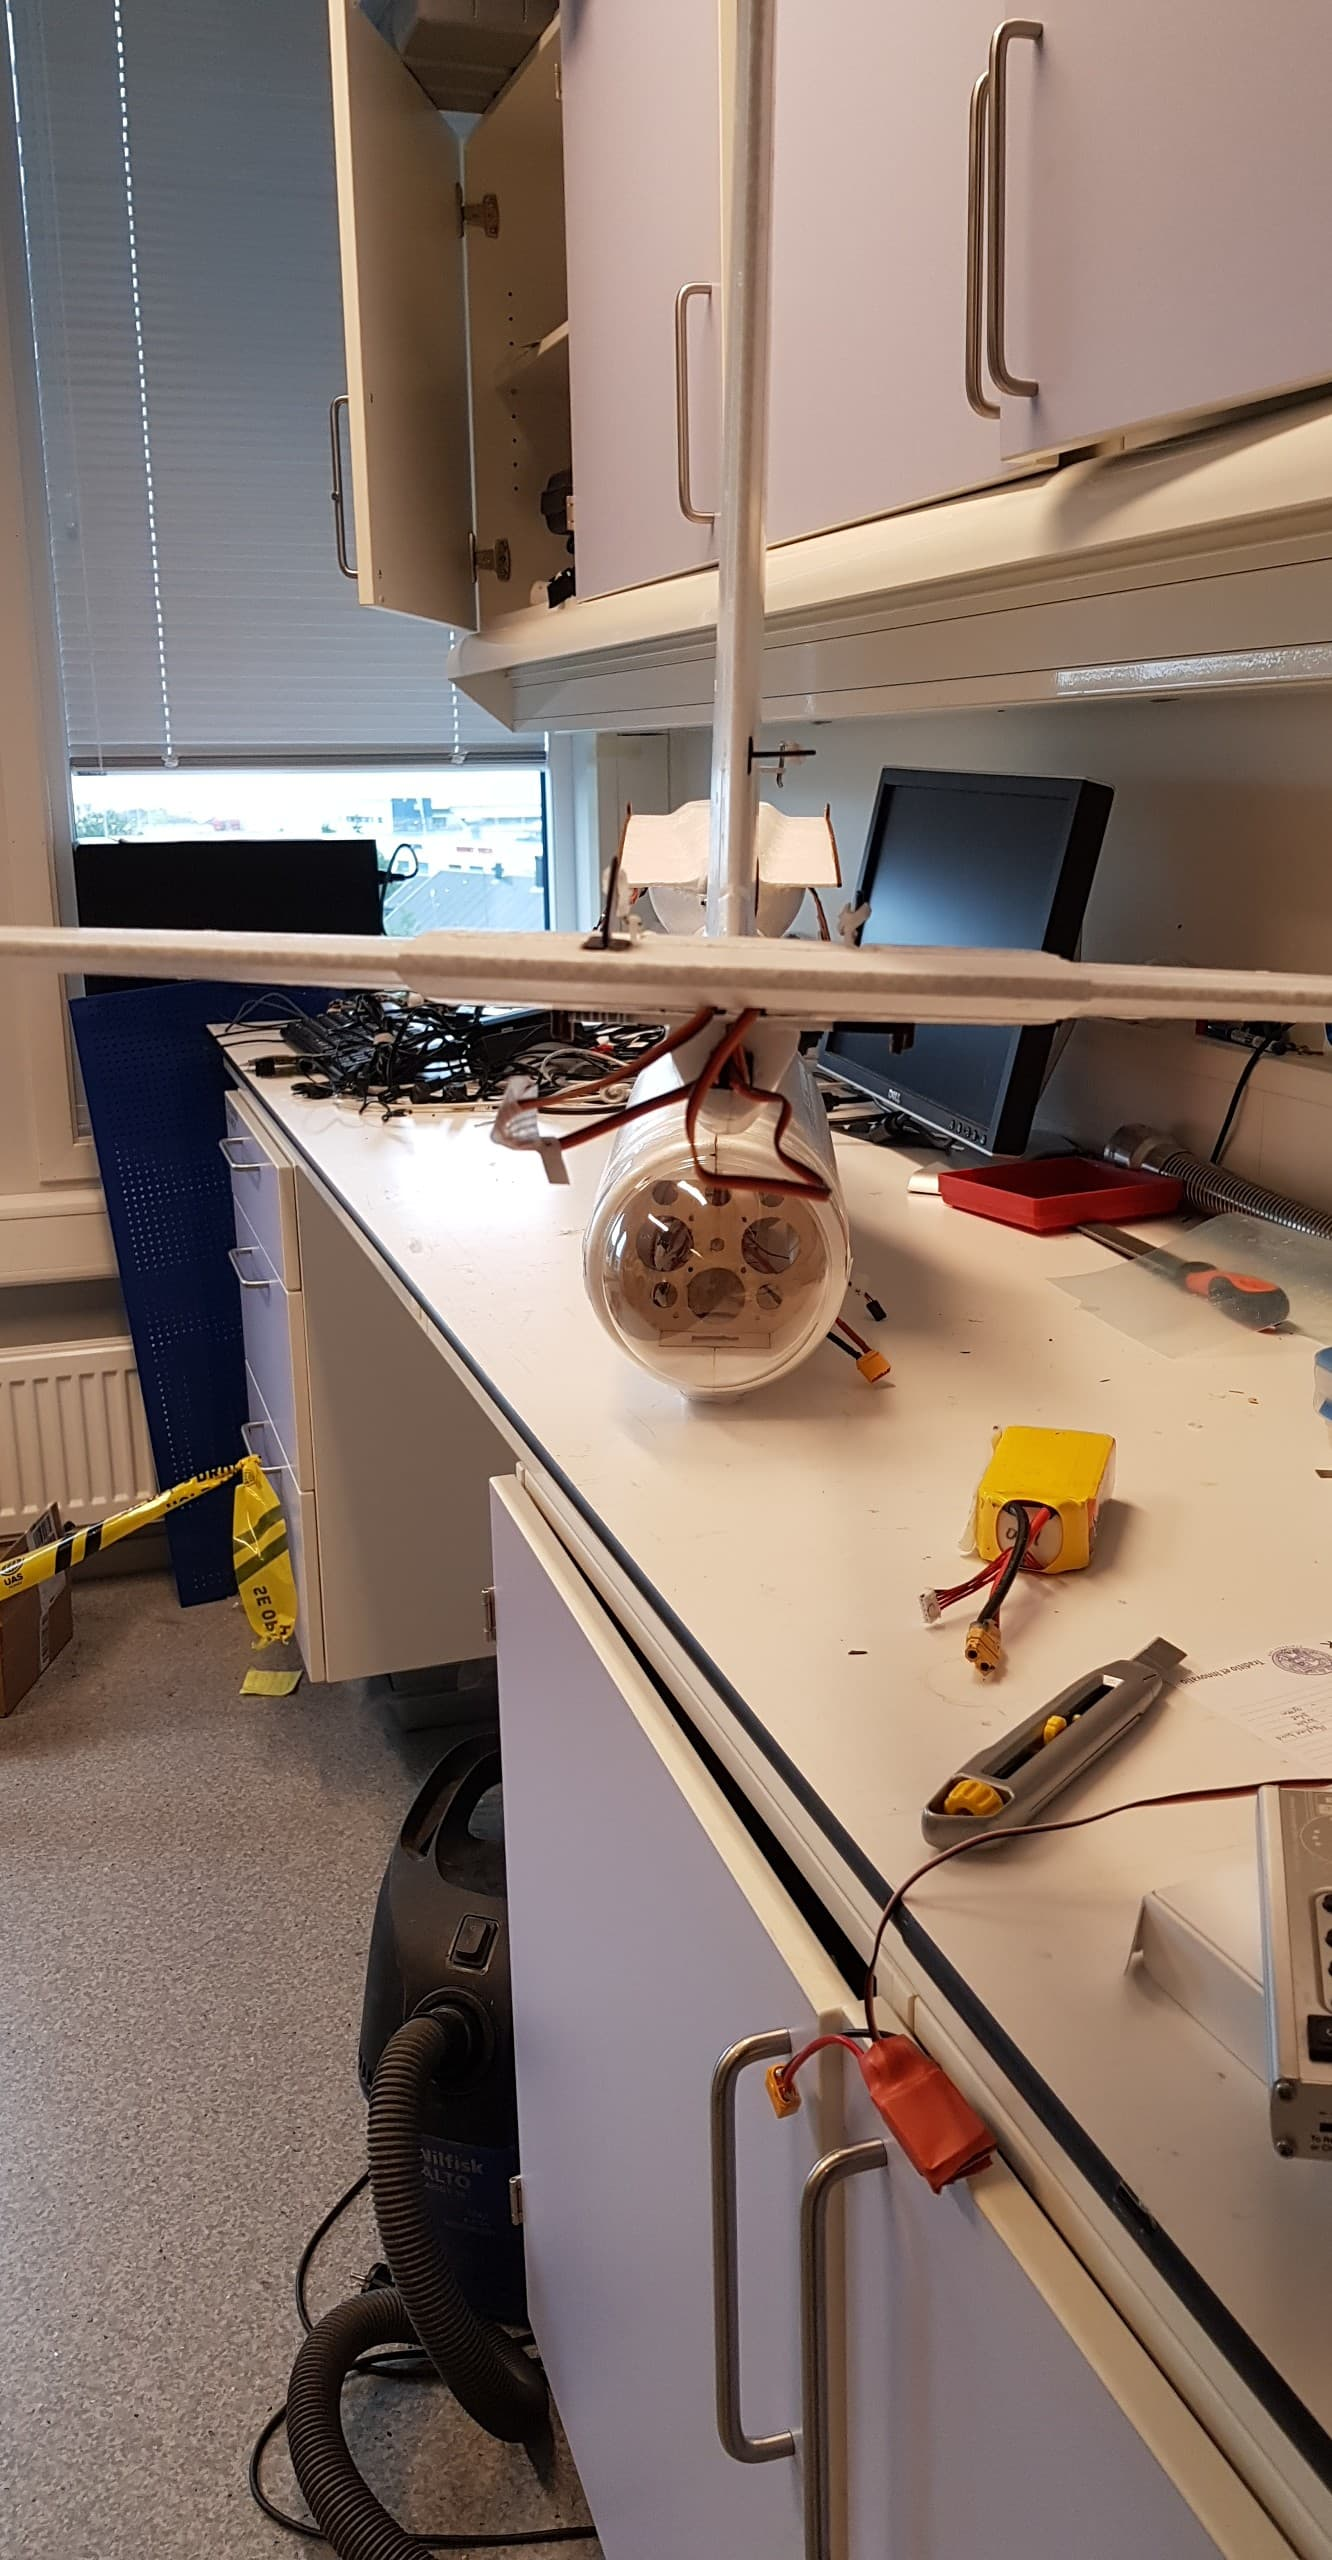
\includegraphics[width = .5\textwidth, height = 10cm]{bilder/skjev_halefinne.jpg}
	\caption[Skjev stabilisator]{Den vertikale stabilisatoren er ikke normal på den horisontale stabilisatoren, og gjør flyging ikke optimalt. Den kan funke, men sideroret må trimmes betraktelig for dette. Det begrenser det totale utslaget.}
\end{figure}

Da det første flyet skulle være en trainer, har den bare det mest nødvendige, altså en RC-link. Alt som måtte da gjøres var å montere mottakeren inni kammeret og koble servokablene til denne. Deretter kalibrere og mappe servo-utgangene, og flyet var klart.

\begin{figure}[ht]
	\centering
	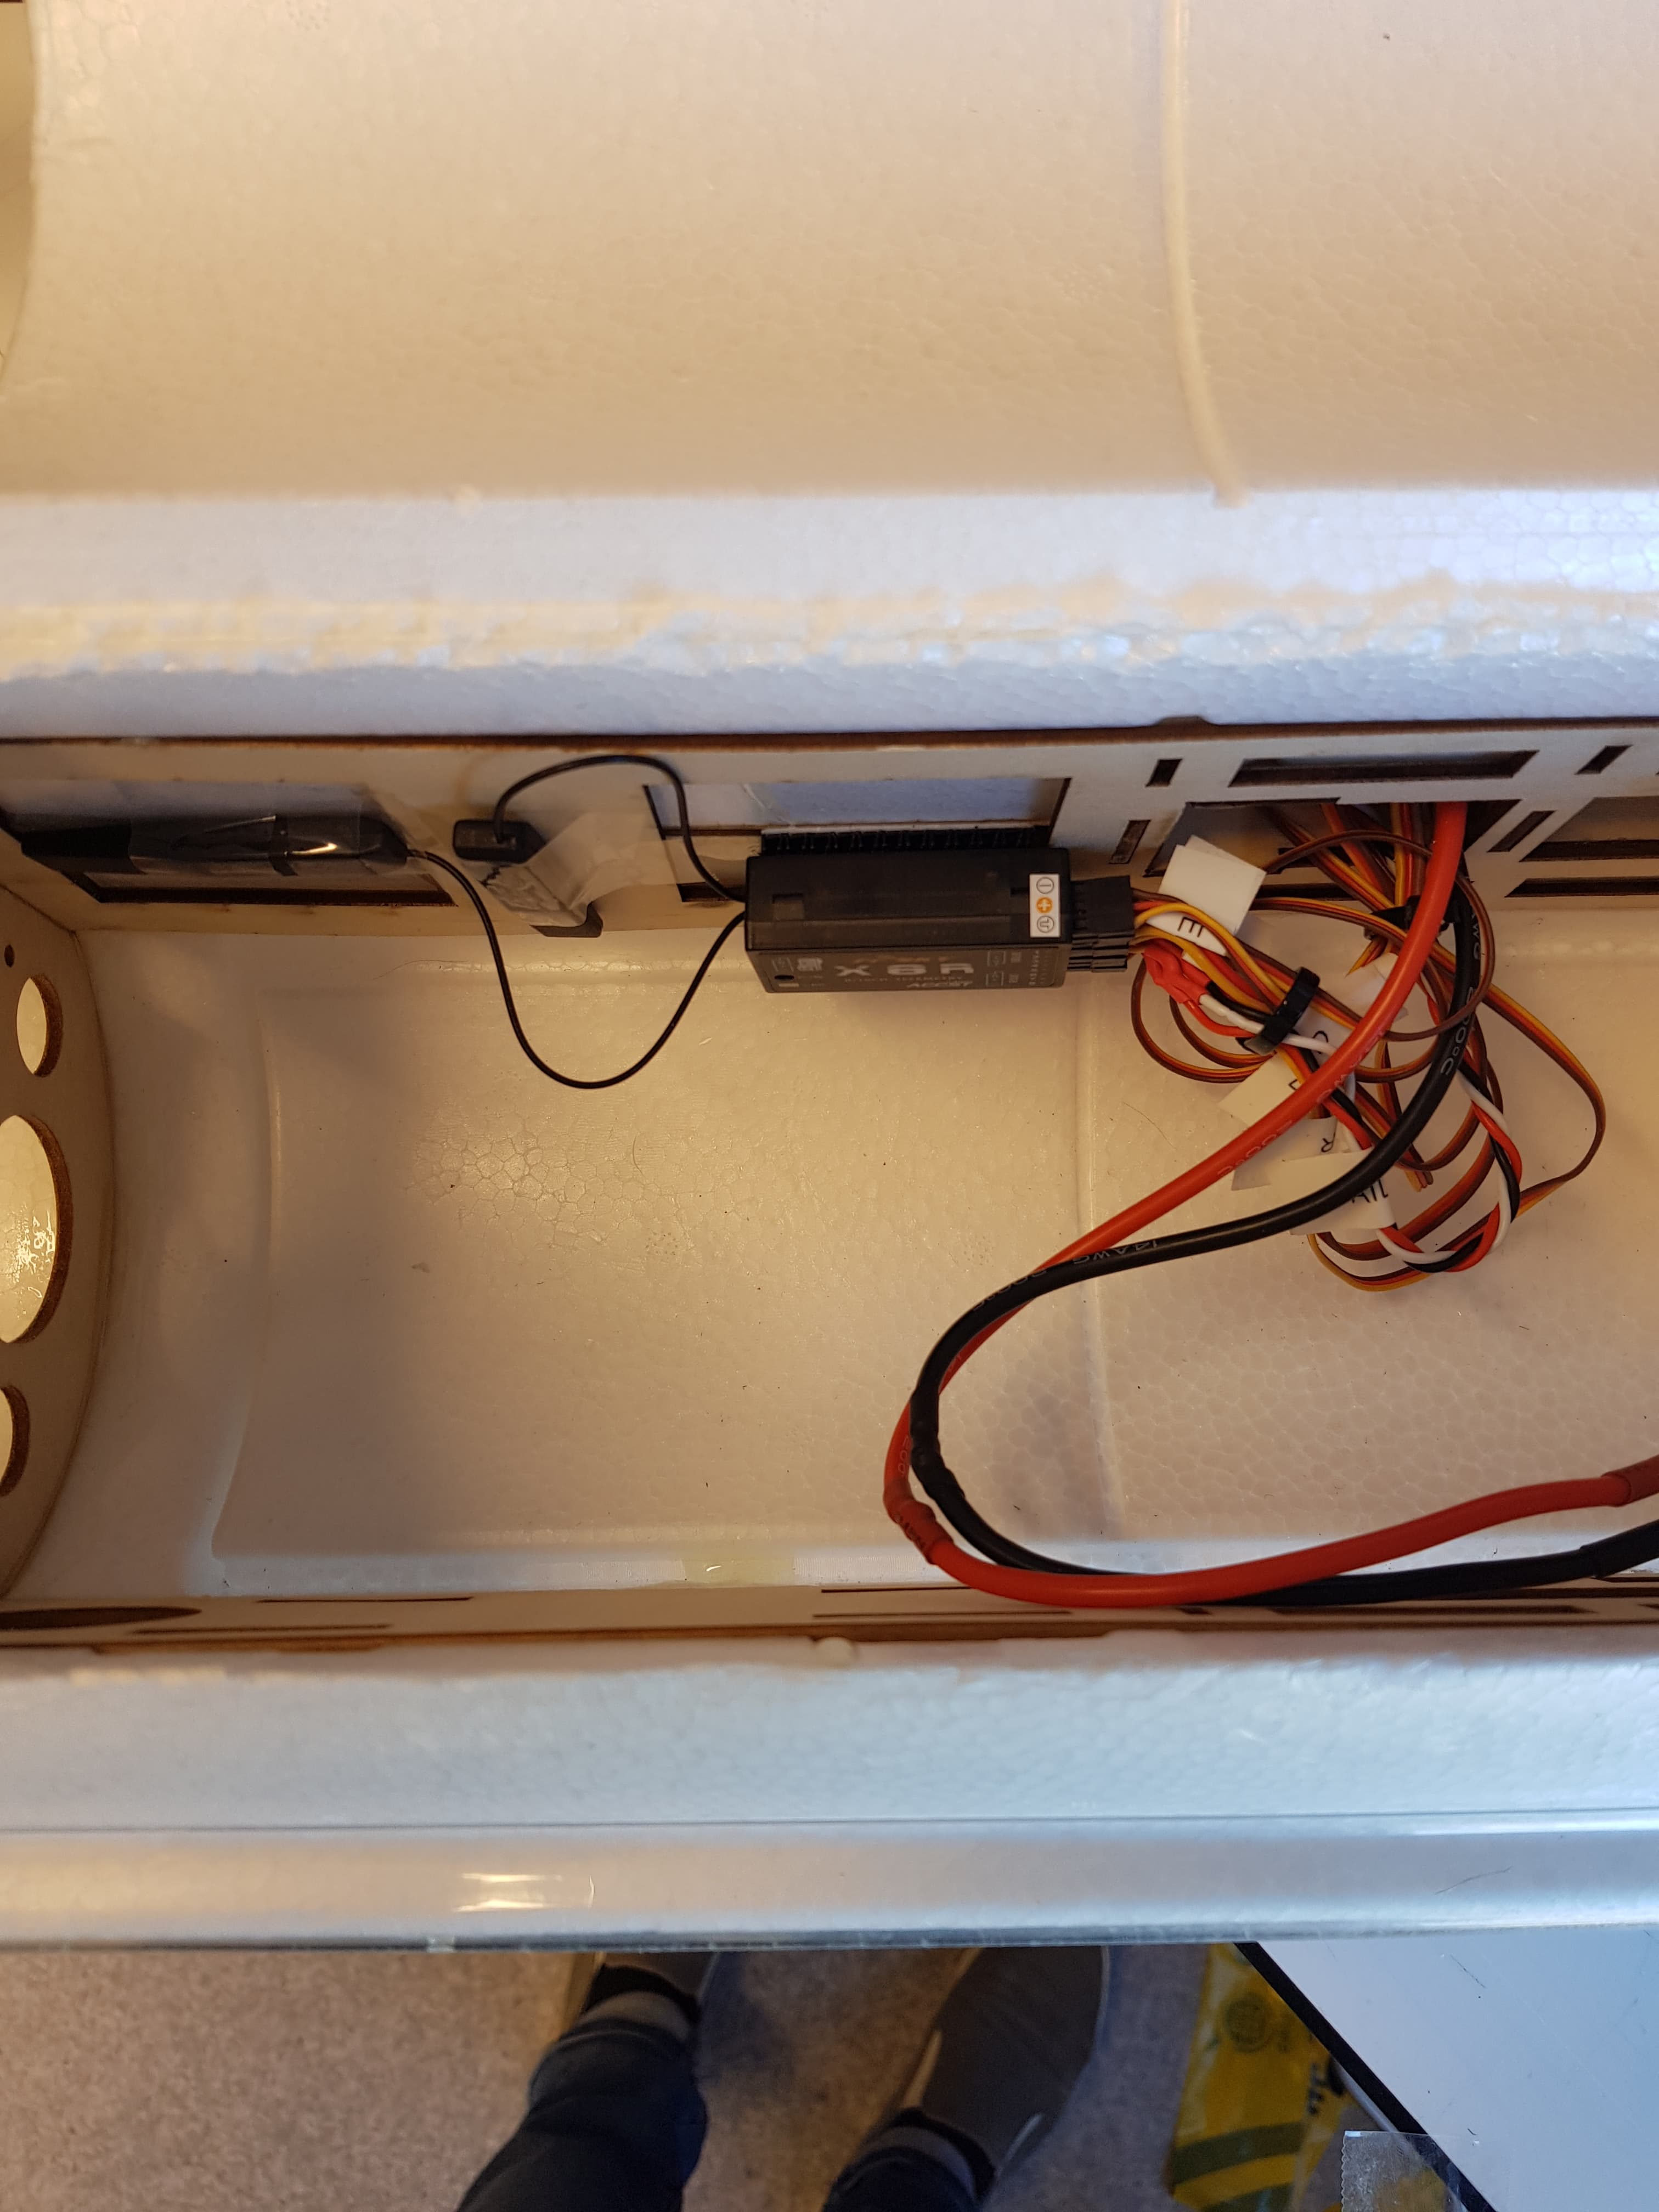
\includegraphics[height=8cm, width = .6\textwidth]{bilder/mottakermontering.jpg}
	\caption[Mottaker-montering]{Ferdig montering av X8R-mottakeren inni Observer-trainer'en. PCB-antennene er plassert i en \ang{90}-orientering for best mulig signalspekter. RC-linken her er PWM-regulert, og benytter én kanal for hver utgang.}
\end{figure}
\newpage

Ved dette oppsettet av RC-linken brukes det totalt 8 kanaler, som er maks antall på denne mottakeren i PWM-konfigurasjon. Alternativt kunne man ha holdt seg til 6 kanaler, der flap-klaffene og balanserorene kobles i parallell. Det uheldige er at da må hver enkelte roroverflate være helt sentrert, slik at bevegelsene er synkron. I tillegg blir det mer jobb med å få servoene til å ``gå riktig vei''. Å holde kanalene uavhengige av hverandre gjør dermed arbeidet mye enklere og oversiktligere. 

\begin{figure}[ht]
	\centering
	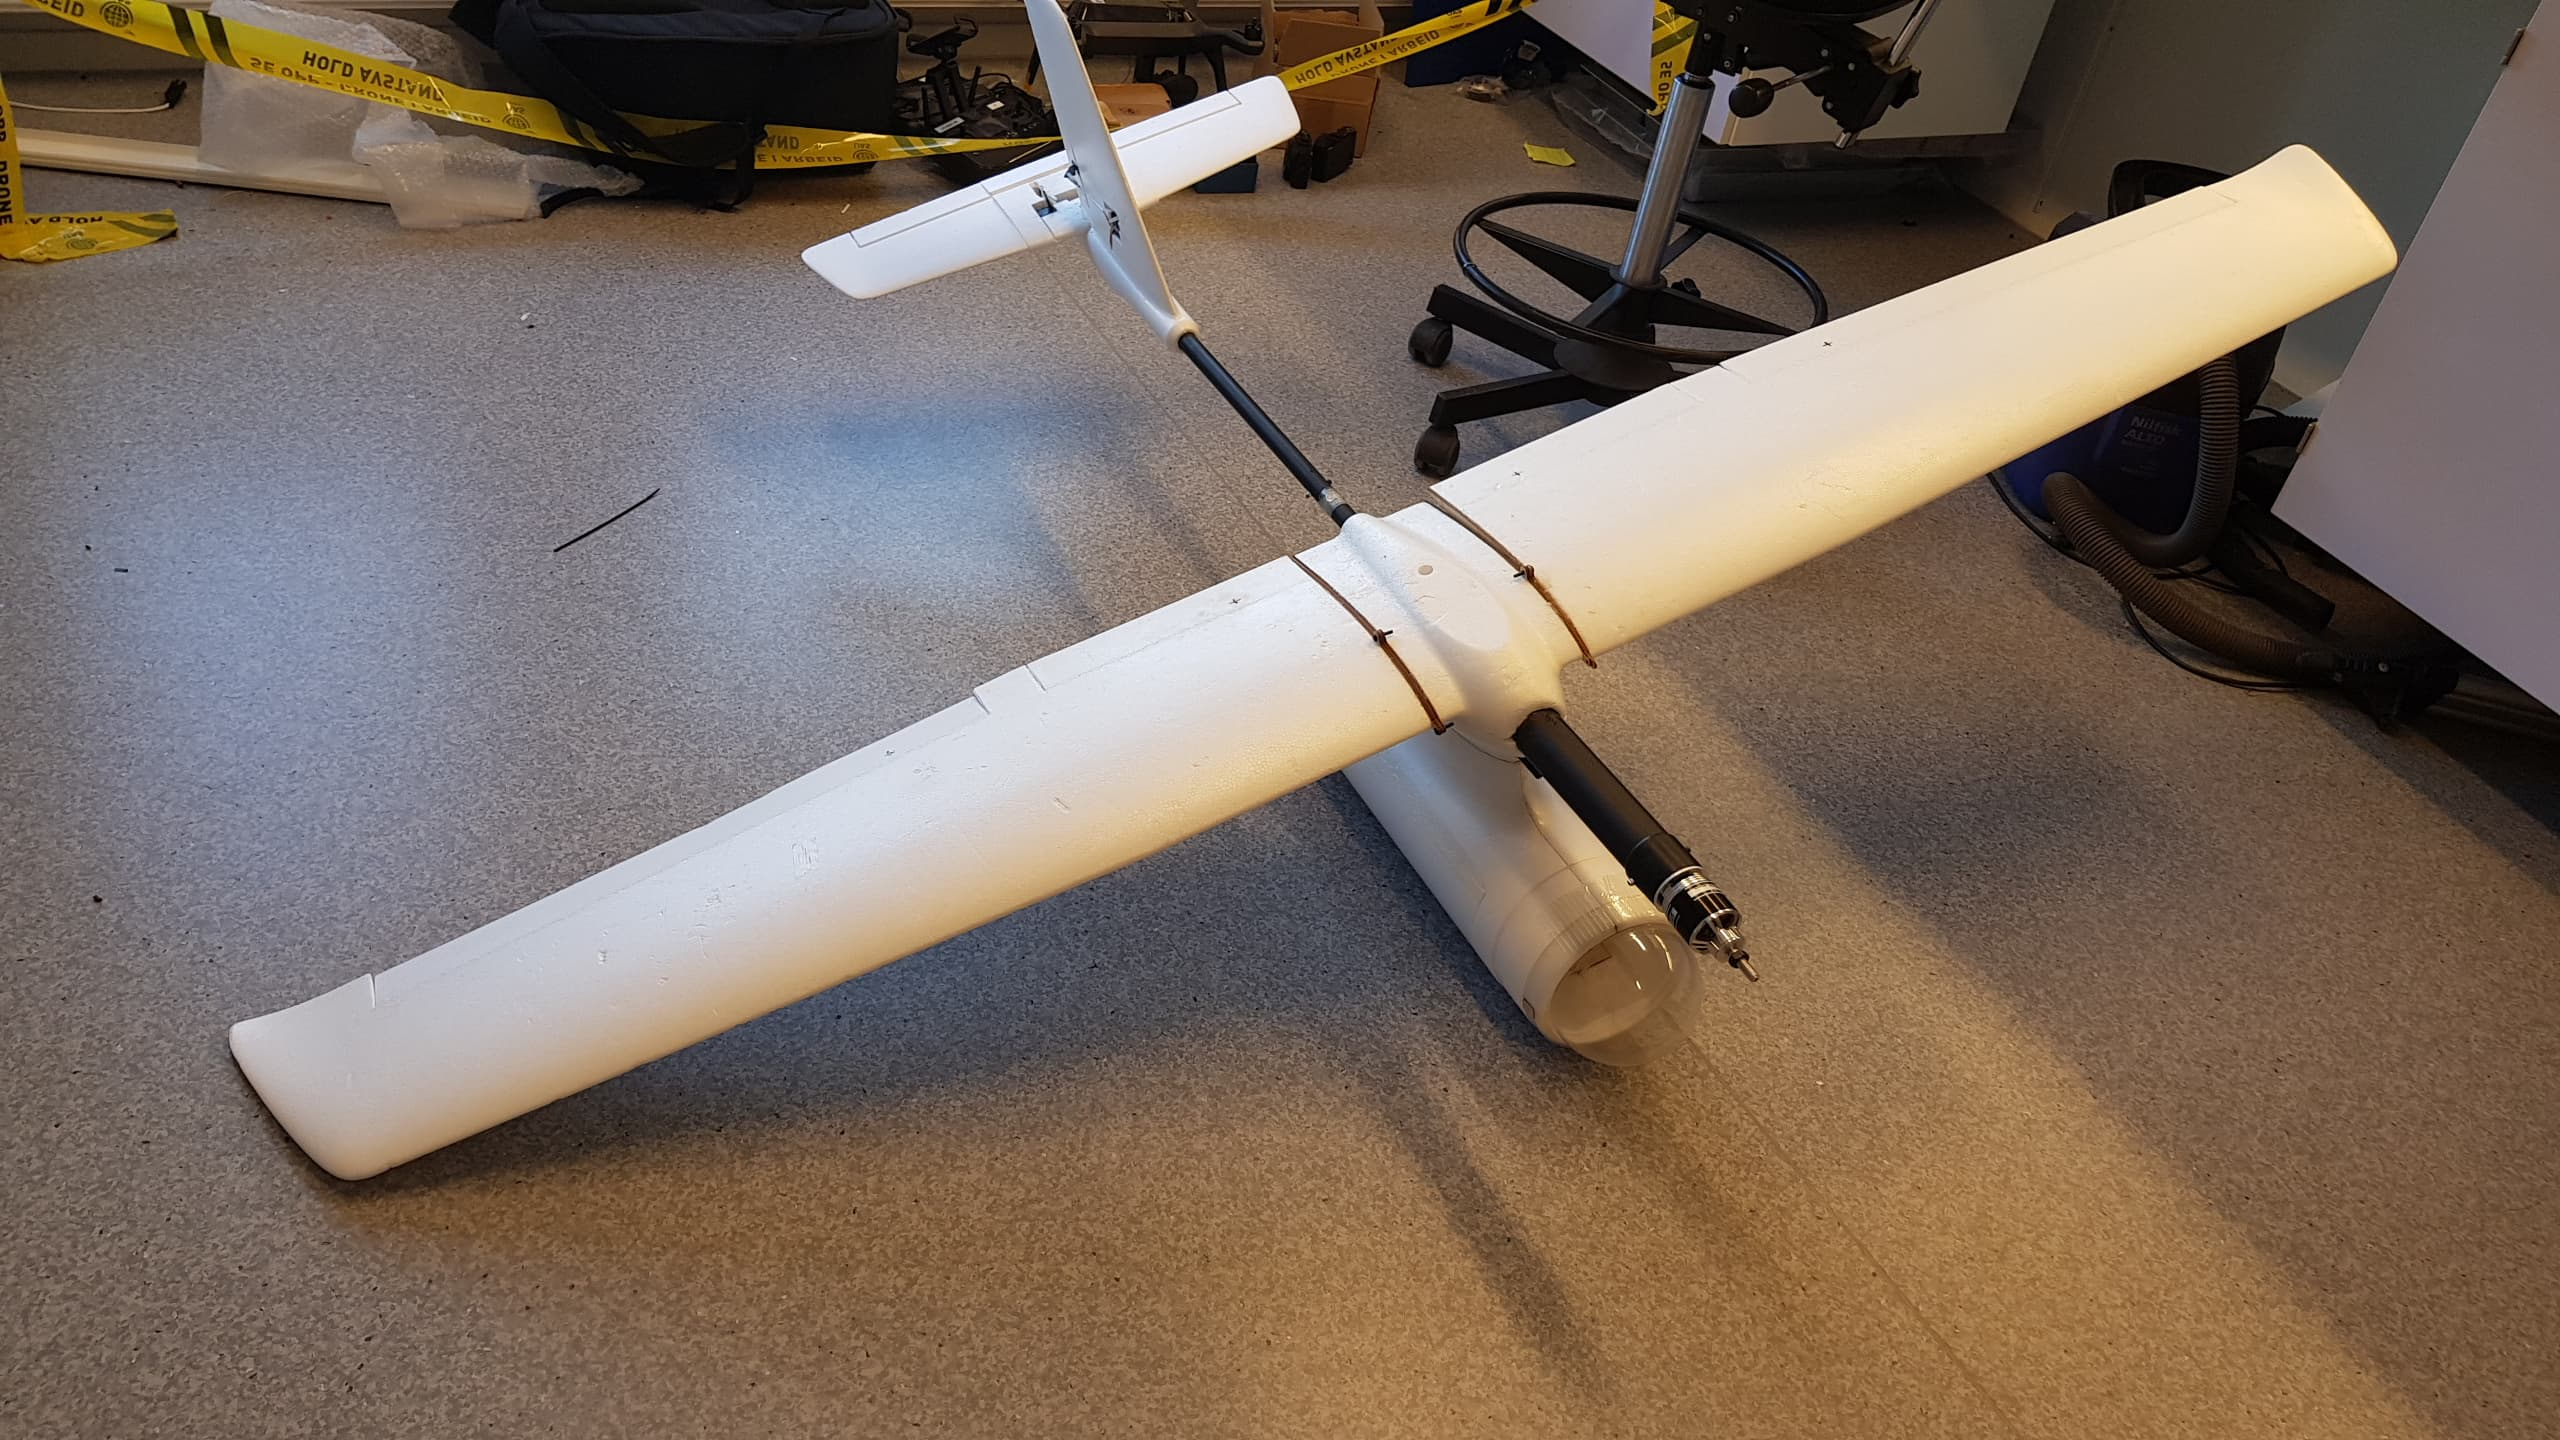
\includegraphics[width=.6\textwidth, height = 6.5cm]{bilder/forste_fly_ferdigstilt.jpg}
	\caption[Trainer-fly]{Trainer - flyet ferdig konfigurert, med vingespenn på 2m, og lengde på 1.5m. Byggingen av denne tok omtrent 1.5 uke. }
\end{figure}

Da jeg hadde fått erfaring av byggingen av den første modellen, gikk det hurtigere å bygge den andre. Med kombinasjon av ``fersk minne'' og noen deler som allerede var ferdiggjort i Bodø, ble nr.2 ferdig på 2 dager. For denne modellen gjenstod å montere og kalibrere servoer på overflatene, kalibrere fartsregulatoren og feste kroppen sammen. Den elektriske sammensetningen fikk jeg ikke gjennomføre, da Norut selv vil gjøre denne delen. Det ble ikke anledning for meg å kunne observere installasjon, da dette skulle tydeligvis gjøres etter endt praksisperiode. \\
Modellen skulle installeres med utstyr for såkalt mapping-formål. Luftfartøyet følger et gridmønster satt opp ved hjelp av en bakkestasjon. Luftfartøyet har forbindelse med bakkestasjonen ved hjelp av en data-link, slik at flyet kan styres utenfor radioens 2.4GHz - rekkevidde. For dette formålet benyttes en Pixhawk - autopilotsystem. I tillegg monteres på ulike sensorer for sikker og koordinert flyging. Dette inkluderer pitot-rør (for hastighetsmåling), spenningssensor, strømsensor og variometer (for høydemåling). 

\begin{figure}[h]
	\centering
	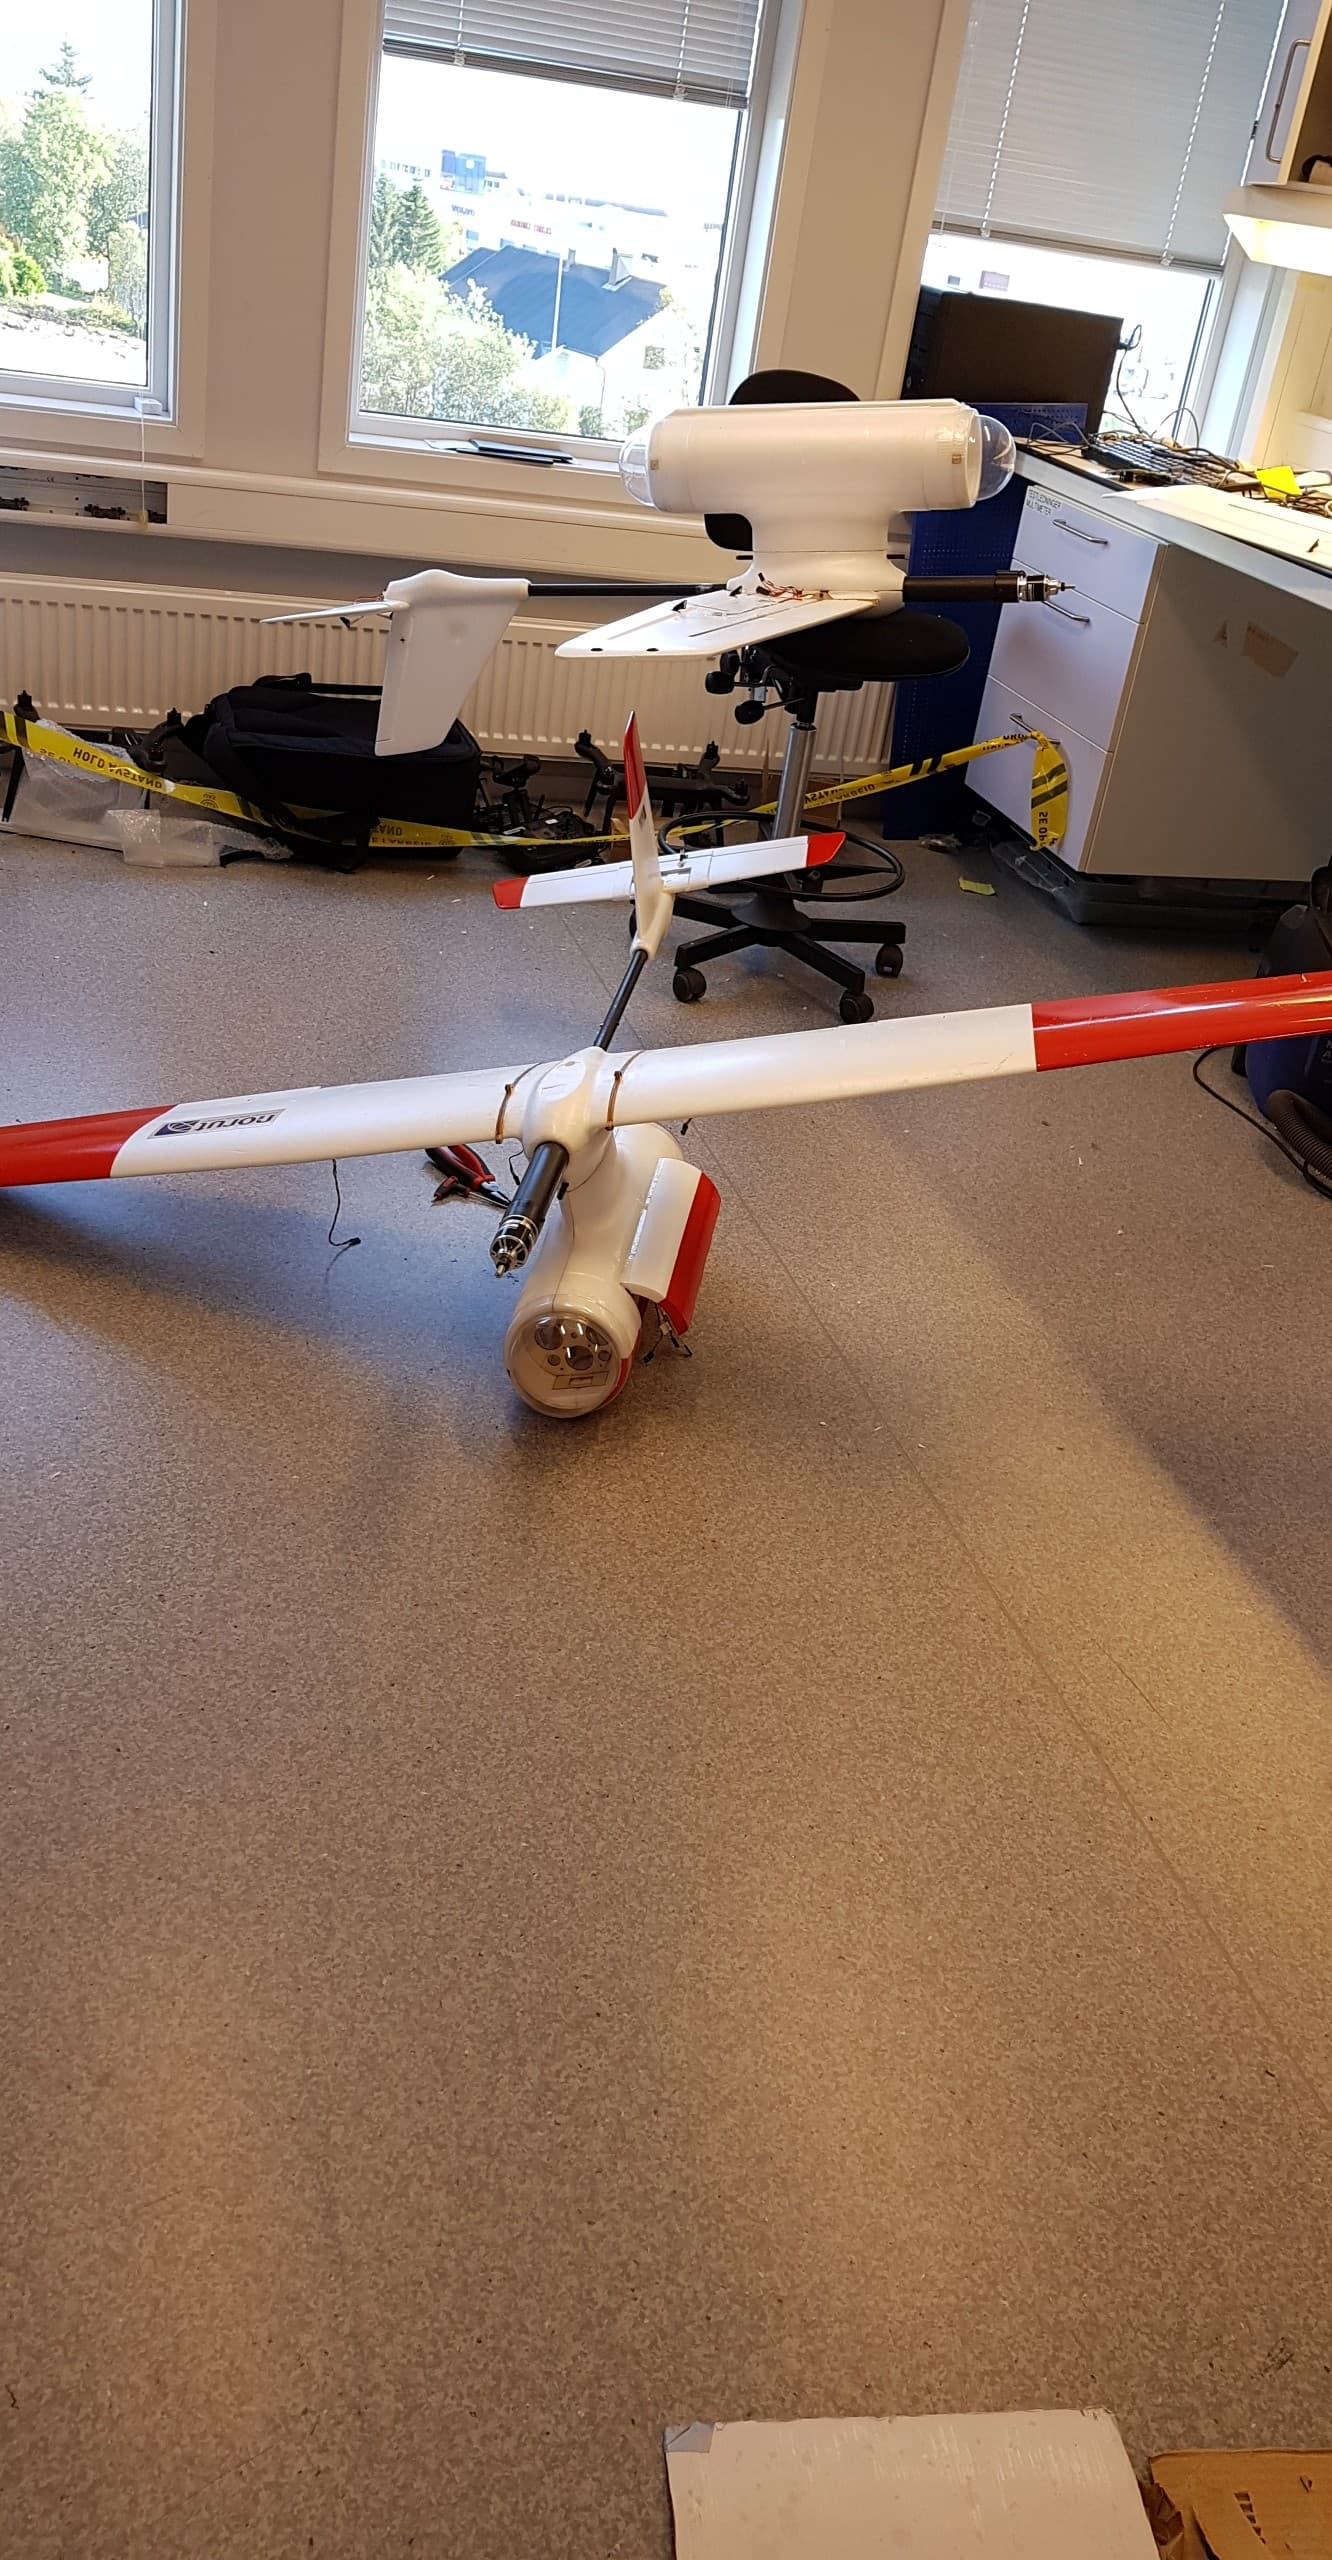
\includegraphics[width = .6\textwidth, height = 8cm]{bilder/andre_fly_ferdigstilt.jpg}
	\caption[Fly nummer to ferdig]{Fly nr. 2 ferdig. Dette skulle monteres med mer avansert utstyr enn traineren i bakgrunnen.}
\end{figure}

\subsubsection{Testflyging}
På den siste arbeidsdagen ble det mulighet for å gjøre testflygning. I forkant av dette ble flyet forberedt til flyging. Servoer sjekkes, eventuelle skader fikses, og flyet monteres. I tillegg må et skjema sendes inn og godkjennes av operativ leder hos Norut. Et slikt skjema kalles for Mission Acceptance Form. Det inneholder opplysninger om den type flyging som skal gjøres, flytype, personell til flyging, risikoanalyser med mer. \\
Da vi ankom til Finnvikdalen for testflygingen gjennomgikk vi monteringen av flyet og  briefet hverandre om take-off og videre flyging. Før take-off begynte vi med en run-up, der vi tester motorens ytelse samt servoenes utslag. Vi oppdaget på run-up at motoren slet etter 
70\%. Vi mistenkte at det hadde noe å gjøre med en usynkronisert fartskontroller eller eventuelle koblingsfeil. Vi ignorerte disse ``varslene'' og bestemte å fortsette. \\
\newpage
Ved take-off skjedde det jeg hadde en mistanke om: Motoren begynte å hakke, og jeg i panikk tok throttelen helt ned, noe som gjorde at flyet steilet på venstre vinge og gikk i bakken. Vi skulle ha tatt hintet og ikke tatt av i det hele, men det er vel slike feil man lærer det meste av. Halen på flyet løsnet og det ene pleksiglasset på kammeret ble knust. 
Hvis ulykken hadde vært mer alvorlig, f.eks personskade, skulle dette rapporteres til Luftfartstilsynet. Det opprettes en ticket og flyet blir holdt på bakken til dette blir fikset. ``Uheldigvis'' var jeg ferdig på praksisperioden min etter denne dagen og fikk dermed ikke muligheten til å fikse disse skadene. Dermed fikk jeg heller ikke muligheten til å føre inn flyets egenskaper i dens POH. 

\newpage
\section{Refleksjon over praksisperioden}
\subsection{Arbeidsforhold}
En ting som jeg oppfattet i løpet av første uke hos Norut, var at det et svært travelt arbeidsmiljø. Norut skulle gjennomføre oppdrag for European Space Agency (ESA), og fokuset av arbeidskraften på UAV-avdelingen gikk for det meste dit.\\
Når jeg fikk hovedoppgaven min, følte jeg at jeg fikk svært begrenset med opplæring. Formelt sett var det ingen opplæring, og oppfølgingen gikk i form av at jeg måtte ta en av ingeniørene til siden og spørre om de hadde tid til å se over hva jeg hadde gjort, eventuelt svare på en del spørsmål. Jeg fikk inntrykket at en del av ingeniørene ``hadde viktigere oppgaver'' å gjøre, og de ga ukomplett veiledning som gjorde meg bare enda mer forvirret og usikker til tider. Oppfølgingen fra Norut var etter min mening ikke noe de tok initiativ til.\\

\begin{figure}[h]
	\centering
	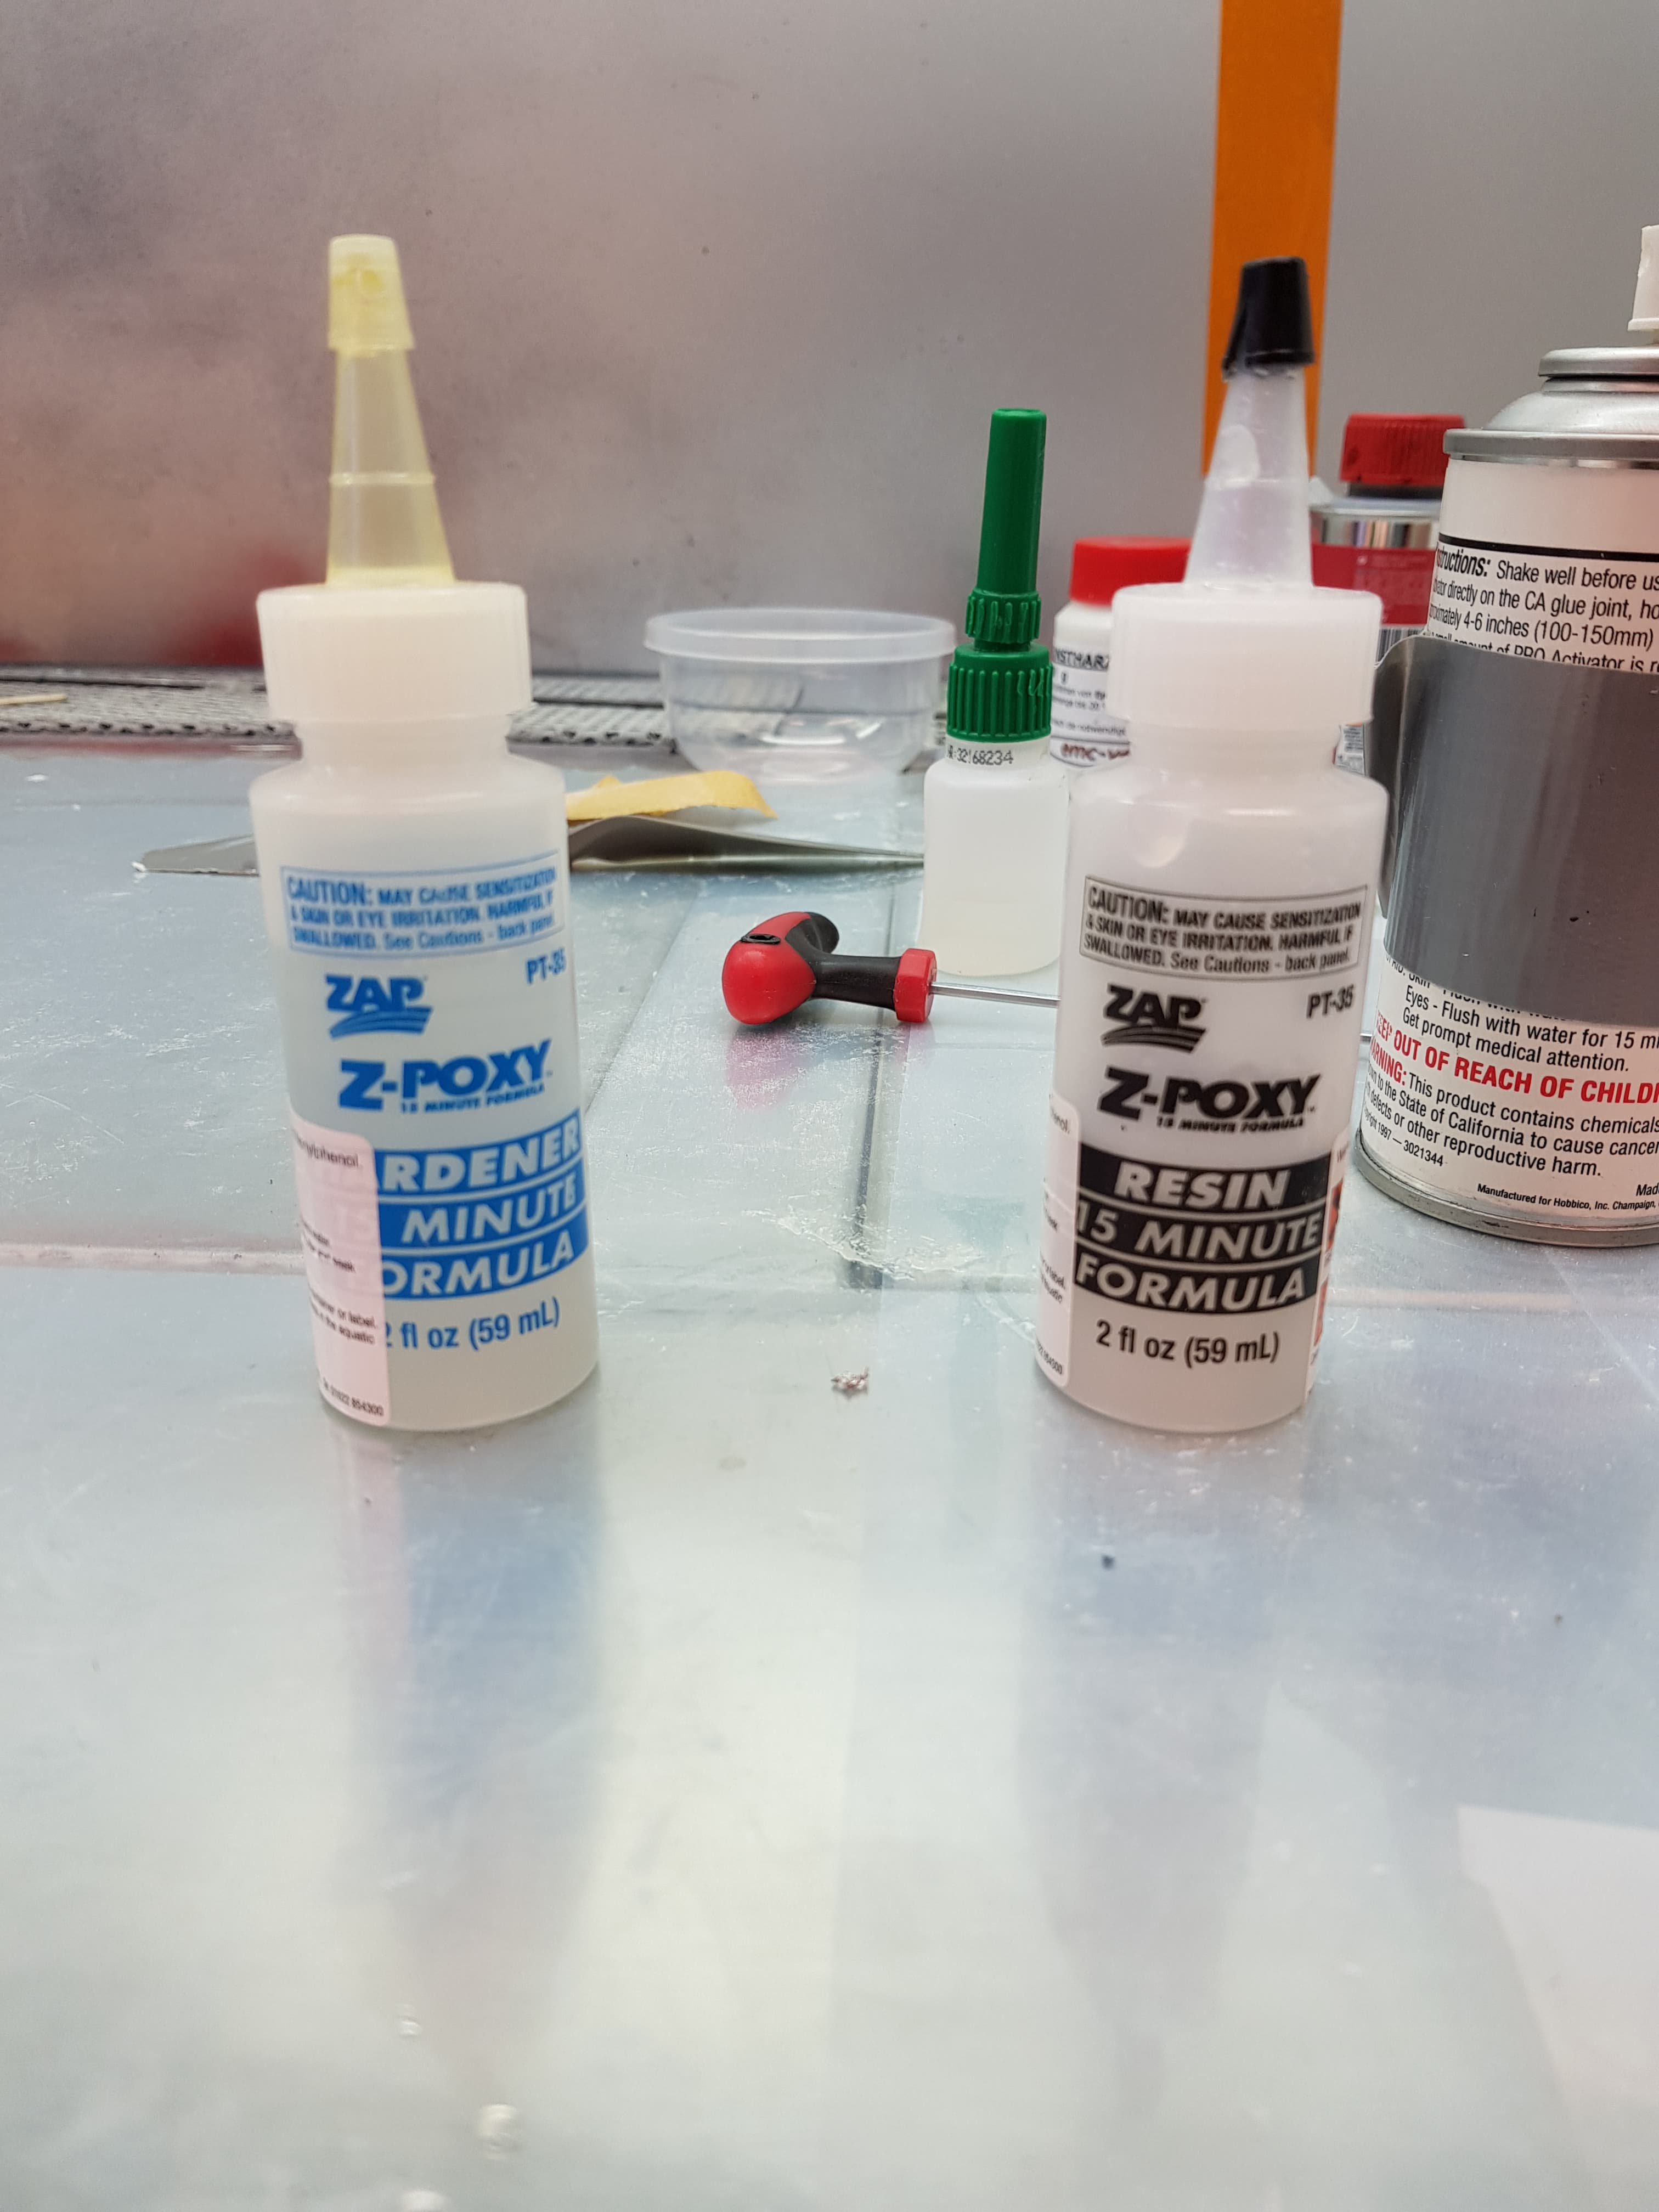
\includegraphics[width = .6\textwidth, height=9cm]{bilder/epoxyresin.jpg}
	\caption[Epoxy og herder]{Epoxy-lim består av to komponenter: resin og herder. Man skal etter Noruts retningslinjer ha opplæring ved bruk av disse stoffene, som inneholder kreftfremkallende stoffer. Svært liten opplæring om bruk og beliggenheter av utstyr i komposittlaben ble gitt. Det var tydeligvis ''underforstått'' at jeg visste hvordan jeg brukte disse stoffene på grunn av forelesninger.}
\end{figure}

Man finner gjerne masse informasjon om bygging av fly på internett, men problemet mitt på dette var at jeg ikke var noe særlig god på praktisk arbeid før jeg begynte hos Norut. Dette gjorde at jeg ble skeptisk og usikker på om det jeg gjorde var faktisk rett. Det faktum at det ikke var noen som passet på at det jeg gjorde var riktig, gjorde at feil lettere slapp gjennom og ikke ble oppdaget før det eventuelt var for sent. Det var heller ingen av ingeniørene som var satt opp til å være en formell kontaktperson under byggingen, enn Rune Storvold. Ting ble dermed fort uorganisert og jeg visste dermed ikke hvem jeg skulle henvende meg for veiledning. \\

Det var satt forutsetninger på ulike punkter, blant annet laging av sjekklister til flyene, noe som jeg ikke fikk vite skulle gjøres på den siste dagen av praksisen. Den ujevne opplysningsstrømmen gjorde at en god del dager ble unødvendig stressende og belastende. 

\subsection{Lærdom}
Til tross for det stressende arbeidsmiljøet fikk jeg lære hvordan man effektivt kan lime ulike materialer med hverandre, samt ulike typer limkompositter. Men jeg kan trygt si at det var lært på den harde måten. Den bakgrunnen jeg har fra emnene jeg har tatt så langt ved universitetet har hjulpet meg innenfor elektronikkforståelsen, men selve håndarbeidet og lignende har jeg erfaring fra hobbybasis. Det er likevel ikke alt som jeg kan ved hjelp av de erfaringene jeg har så langt ta beslutninger på. Et eksempel er liming av ulike materialer til hverandre. Med andre ord, hvordan limstruktur som passer best, og hvordan man får best mulig fysisk binding mellom materialene. Mye av dette lærte jeg ved å lese på hobby-forum om hvordan andre har brukt ulike limsorter til ulike formål. \\
Skolen gjør en ikke helt forberedt til arbeidslivet, noe som kan gjøre hoppet mellom skolebenken og jobb vanskelig. Jeg har i hvert fall fått lært at læringen stopper ikke etter utdannelsen. Den virkelige læringen kommer ute i arbeidslivet. 

\section{Konklusjon}
Læringsmålet for min prakisperiode har jeg beskrevet til å være å få et inntrykk av en typisk arbeidsdag for en ingeniør. Ved hjelp av kunnskapen jeg hadde og den jeg opparbeidet meg under praksisen, klarte jeg å fremstille to fly på bestilling av Norut. Jeg har lært mye nyttig som jeg kan ta videre til andre prosjektoppgaver og arbeidsutfordringer i løpet av min yrkeskarriere. \\
En del ting kunne ha blitt gjort bedre for at perioden skulle vært mer organisert. En person med mindre til ingen erfaring i bygging, lodding eller annet praktisk arbeid ville etter min mening ha slitt med denne oppgaven. Likevel synes jeg det var moro og lærerikt å få bygge (mine første) ubemannede fixed-wings. \\
Å ha praksis som valgmemne vil jeg si var svært lurt, da man får den reelle smakebiten av en typisk ingeniørs arbeidsdag. Det samme får man bare ikke ved å sitte på skolebenken. Da jeg er av en mer teoretisk karakter enn praktisk, hjalp det veldig å oppleve dette. All kunnskapen jeg har opparbeidet meg gjennom perioden vil være nyttig til senere tider. 
\clearpage


\section{Vedlegg}
I dette kapittelet finner du følgende som kan være interessant å se.\\

\begin{enumerate}
	\item Attest fra Norut
	\item Beskrivelse av praksis for TEK-2000
	\item Logg av praksisperioden
	\item CryoWing Observer RC-trainer byggelogg
	\item Determining capabilities for CryoWing Observer
		\item CryoWing Observer Pilot Operating Handbook
\end{enumerate}

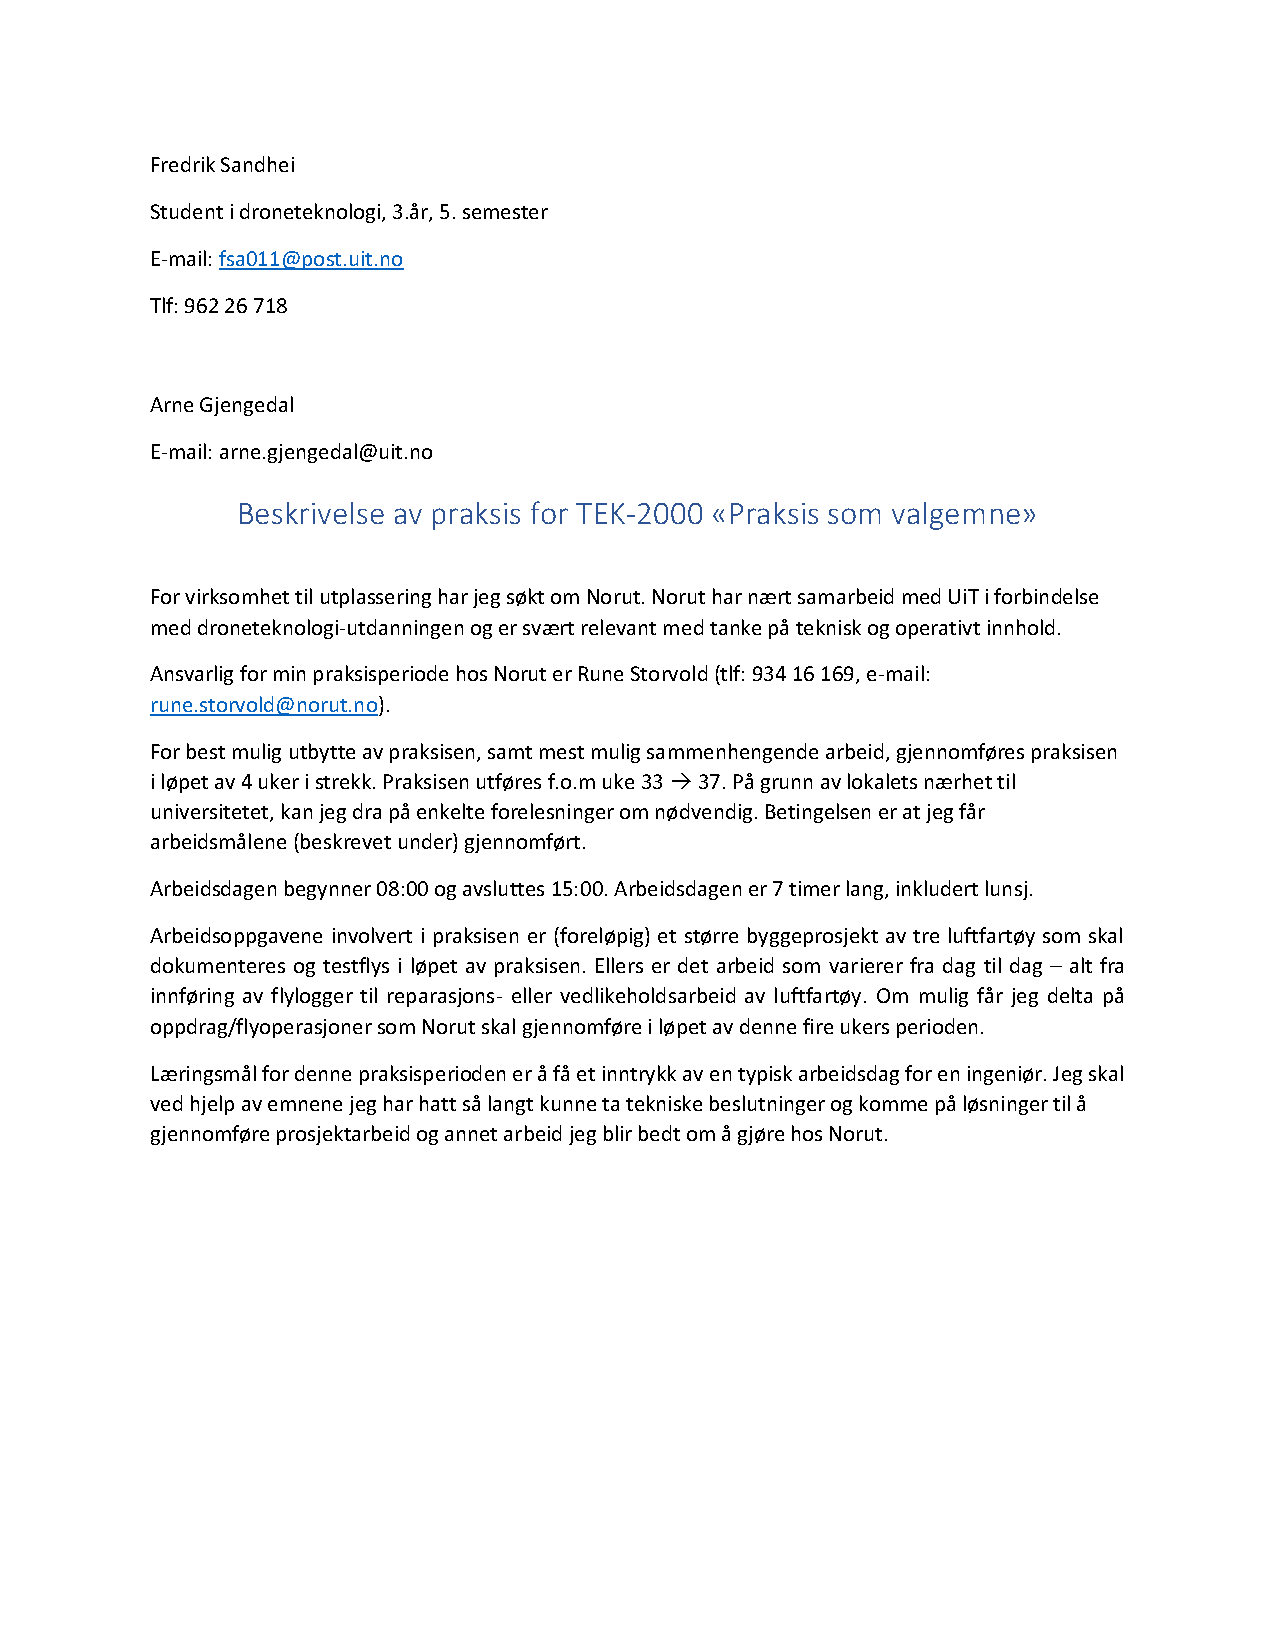
\includepdf[pages=-]{vedlegg/Beskrivelse_av_praksis_for_TEK.pdf}
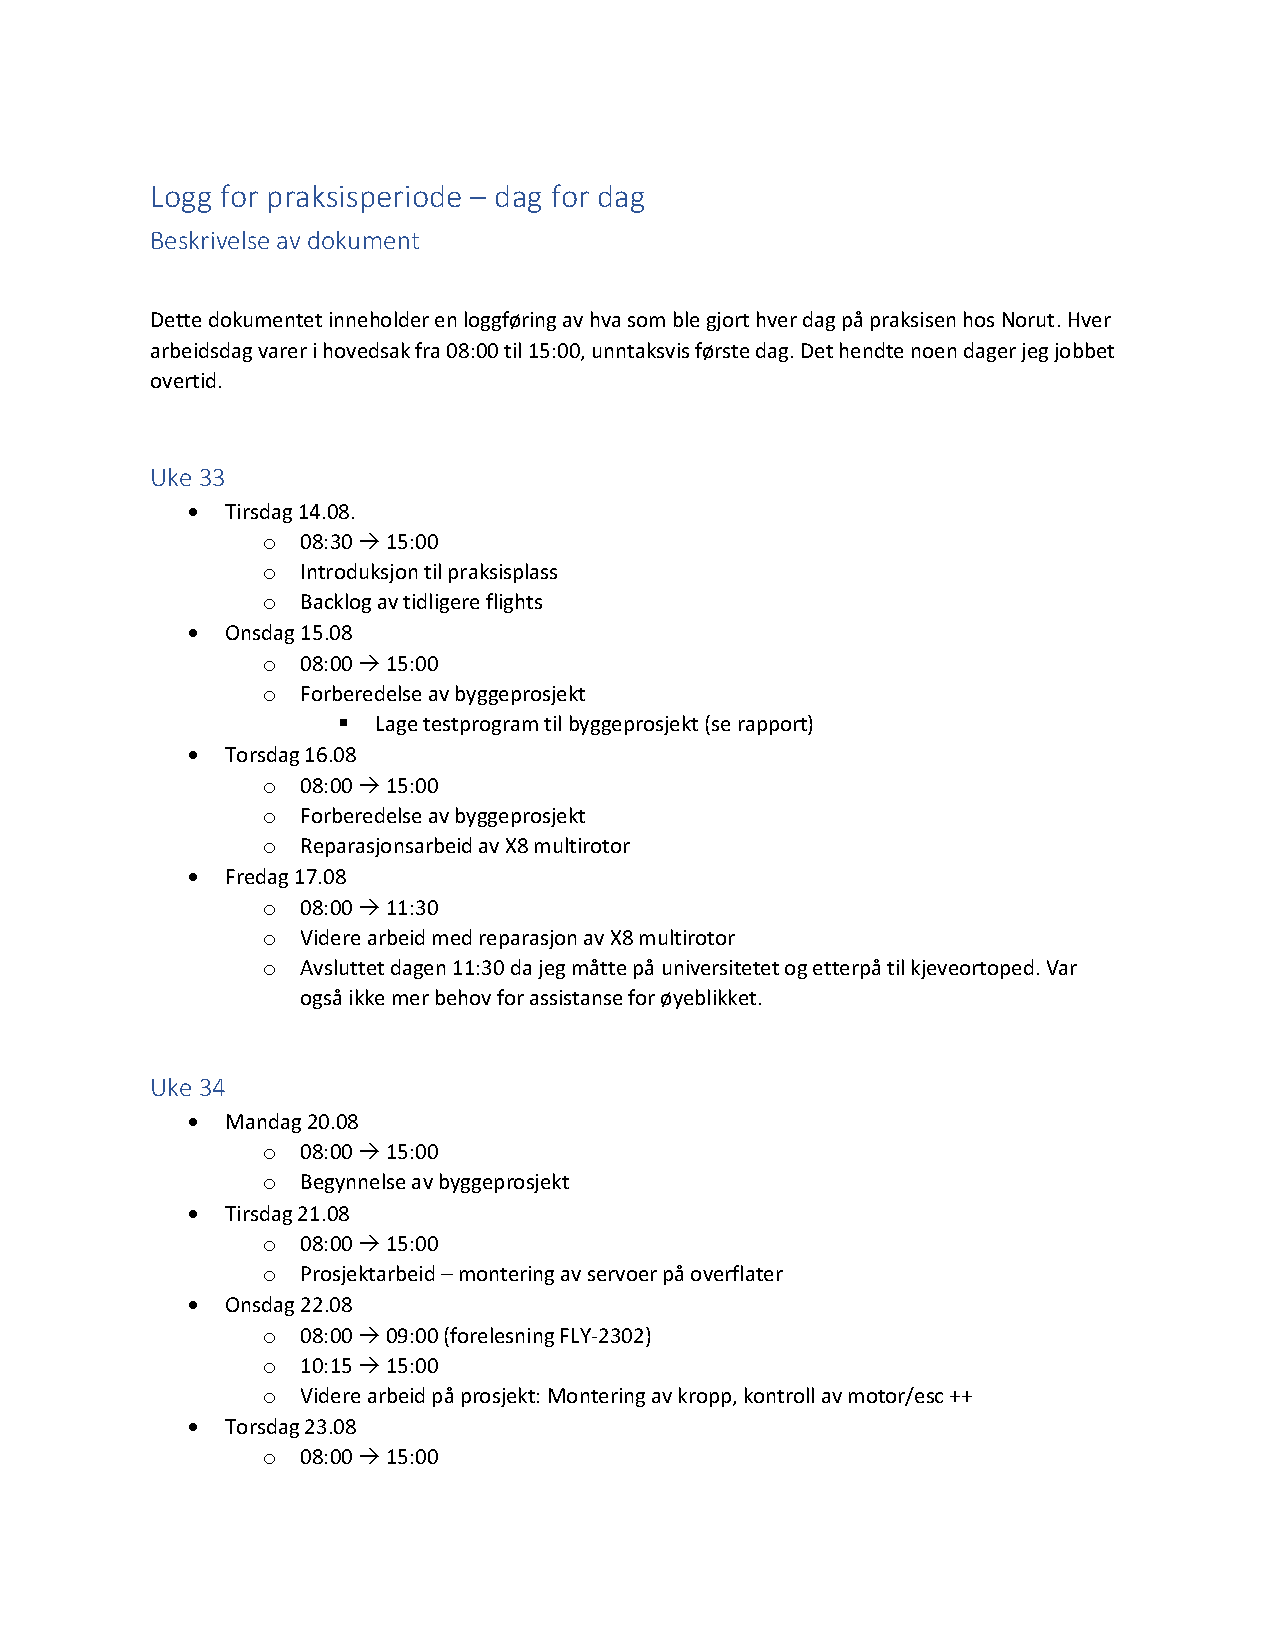
\includepdf[pages=-]{vedlegg/Logg_av_praksisperiode.pdf}
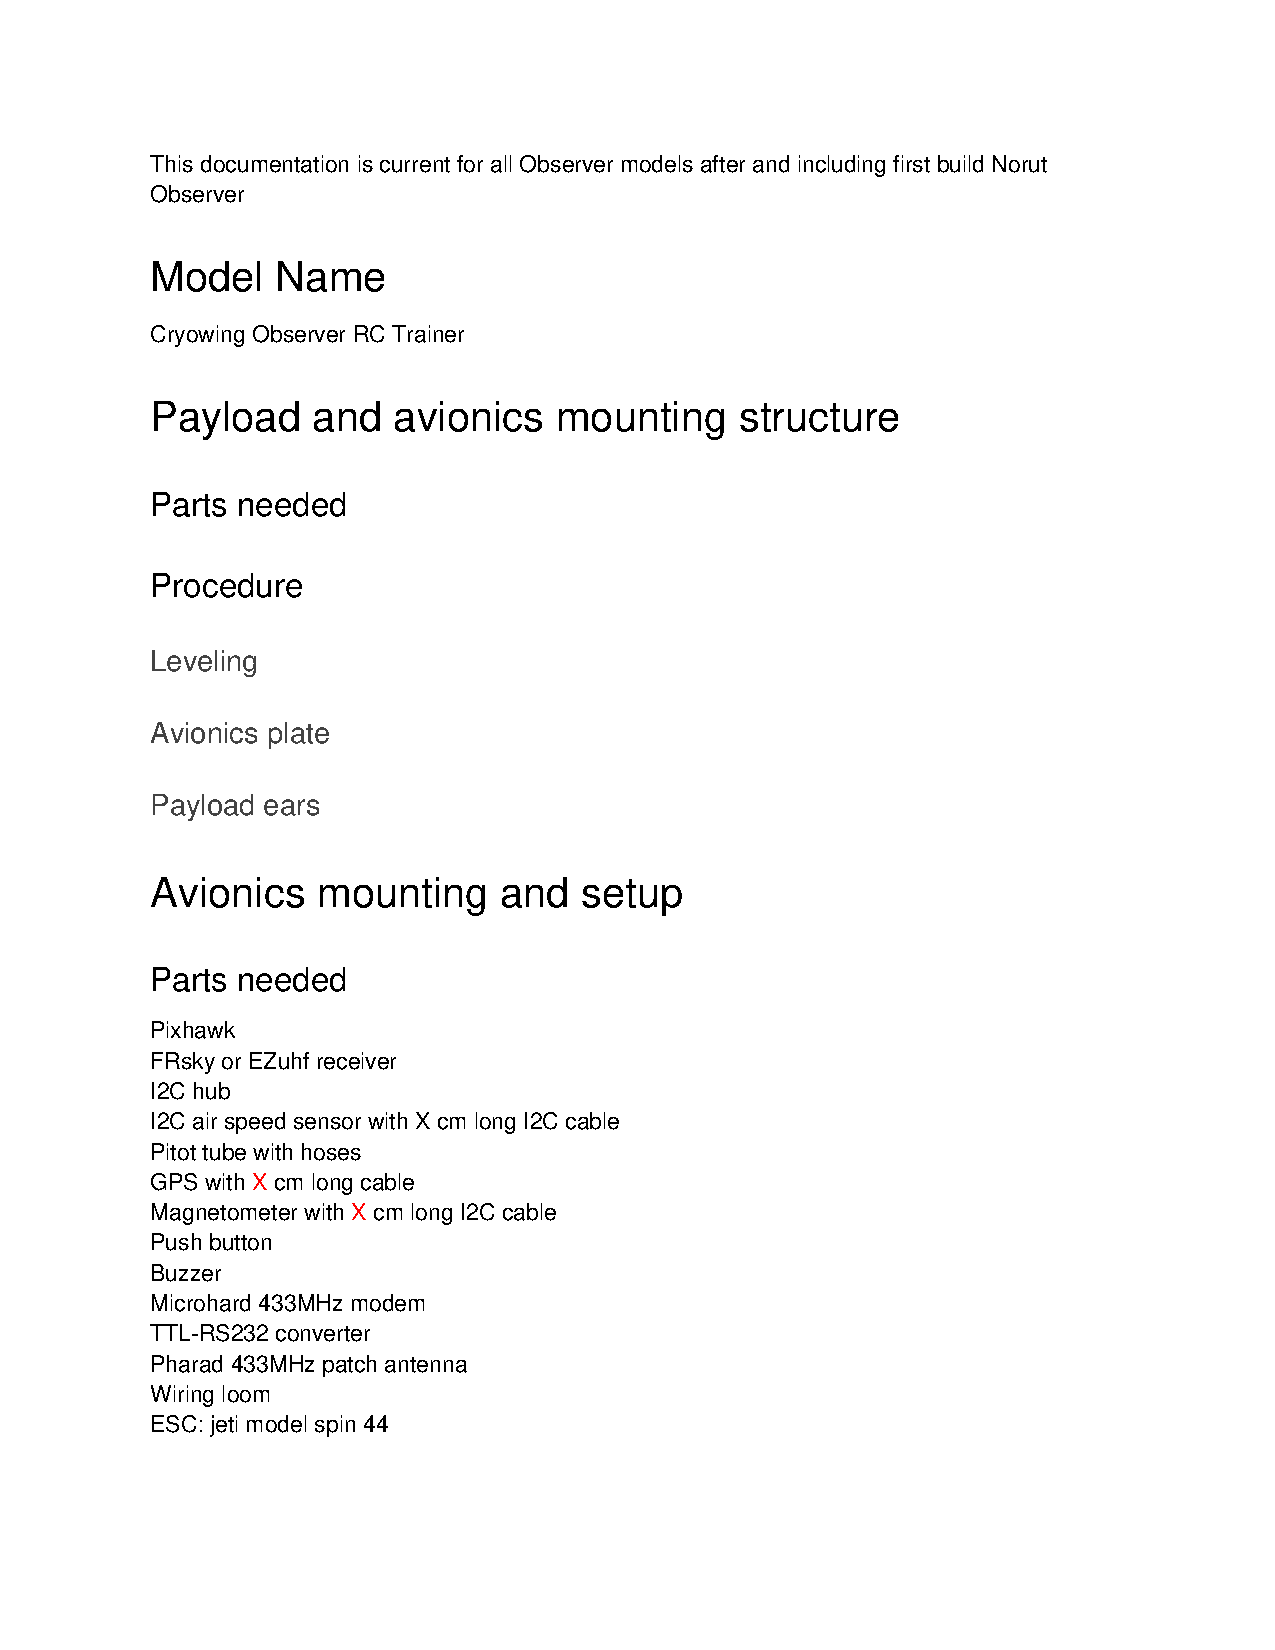
\includepdf[pages=-]{vedlegg/Observer_RC_Trainer_build_documentation.pdf}
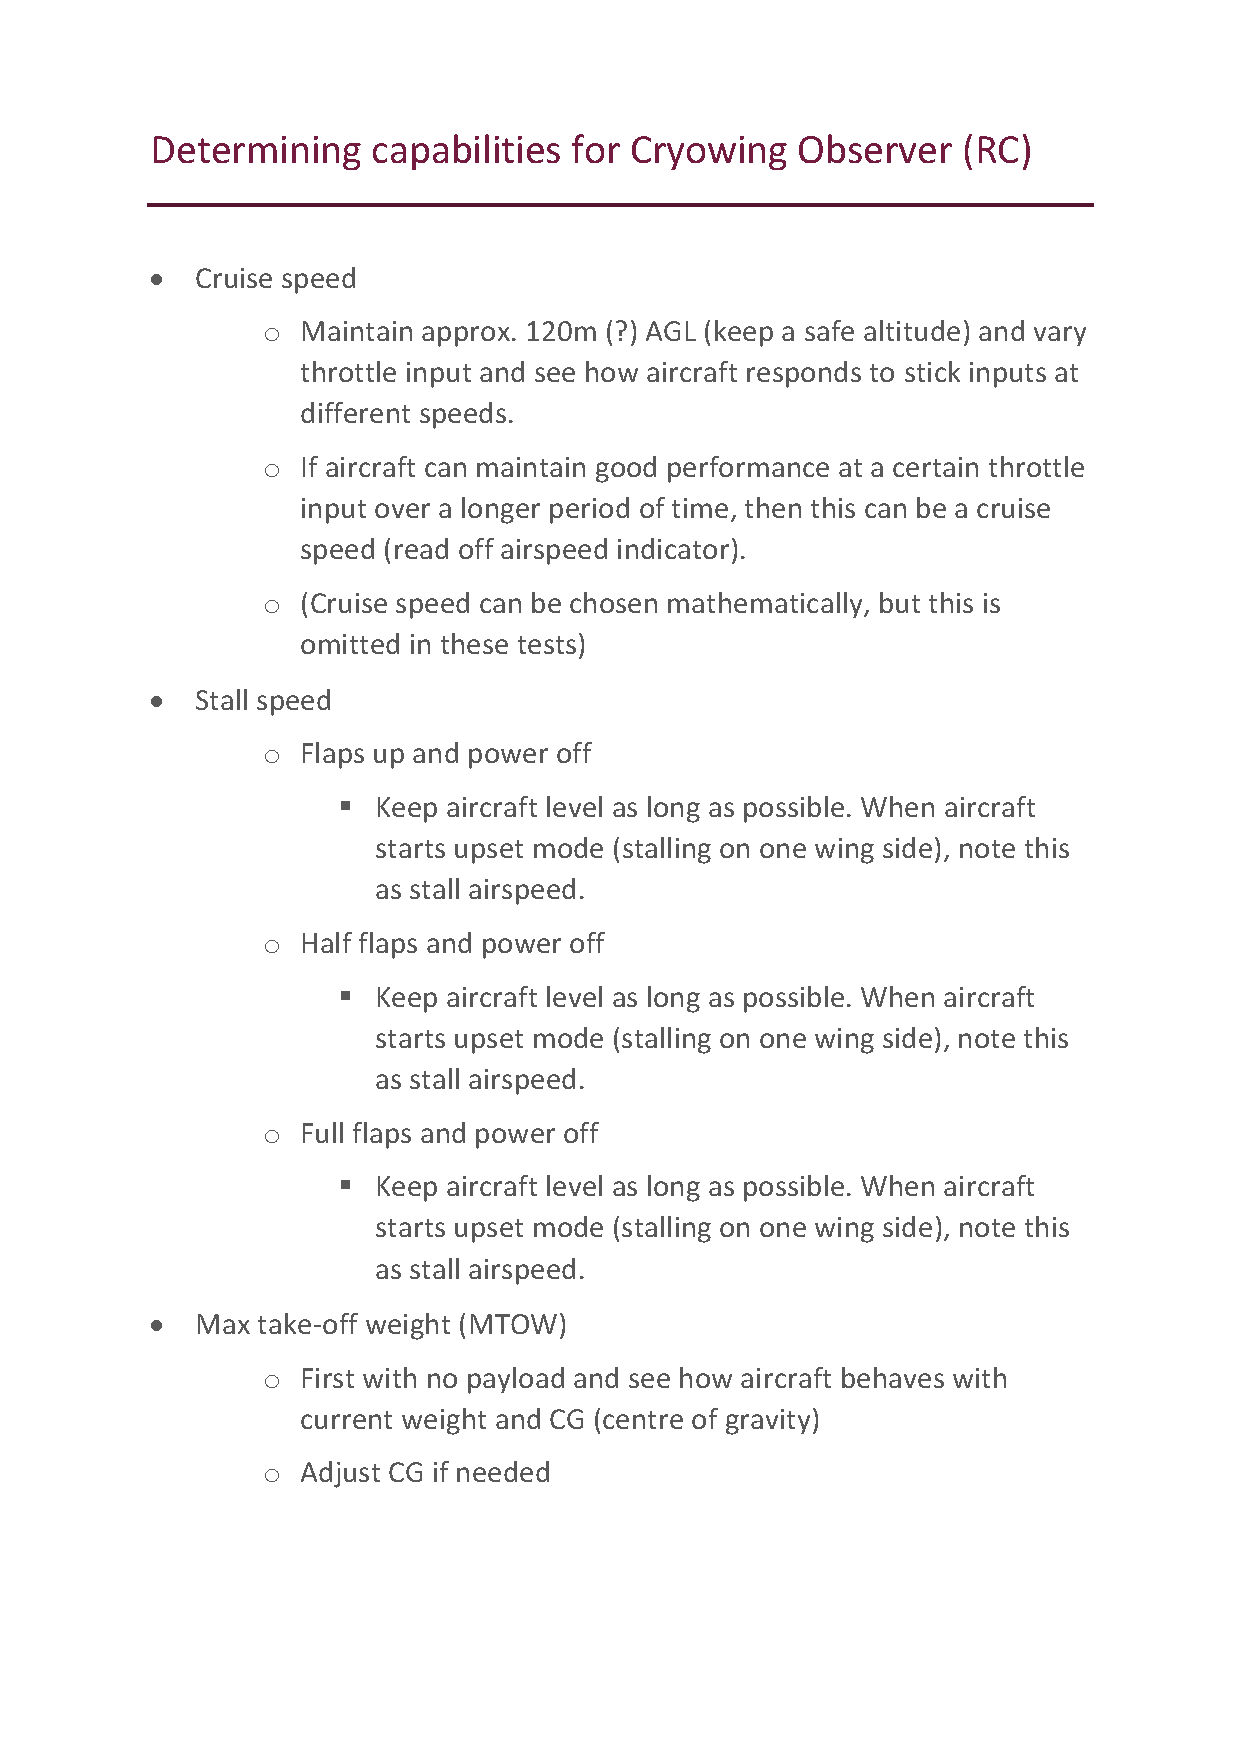
\includepdf[pages=-]{vedlegg/Determining_capabilities_for_Cryowing_Observer.pdf}
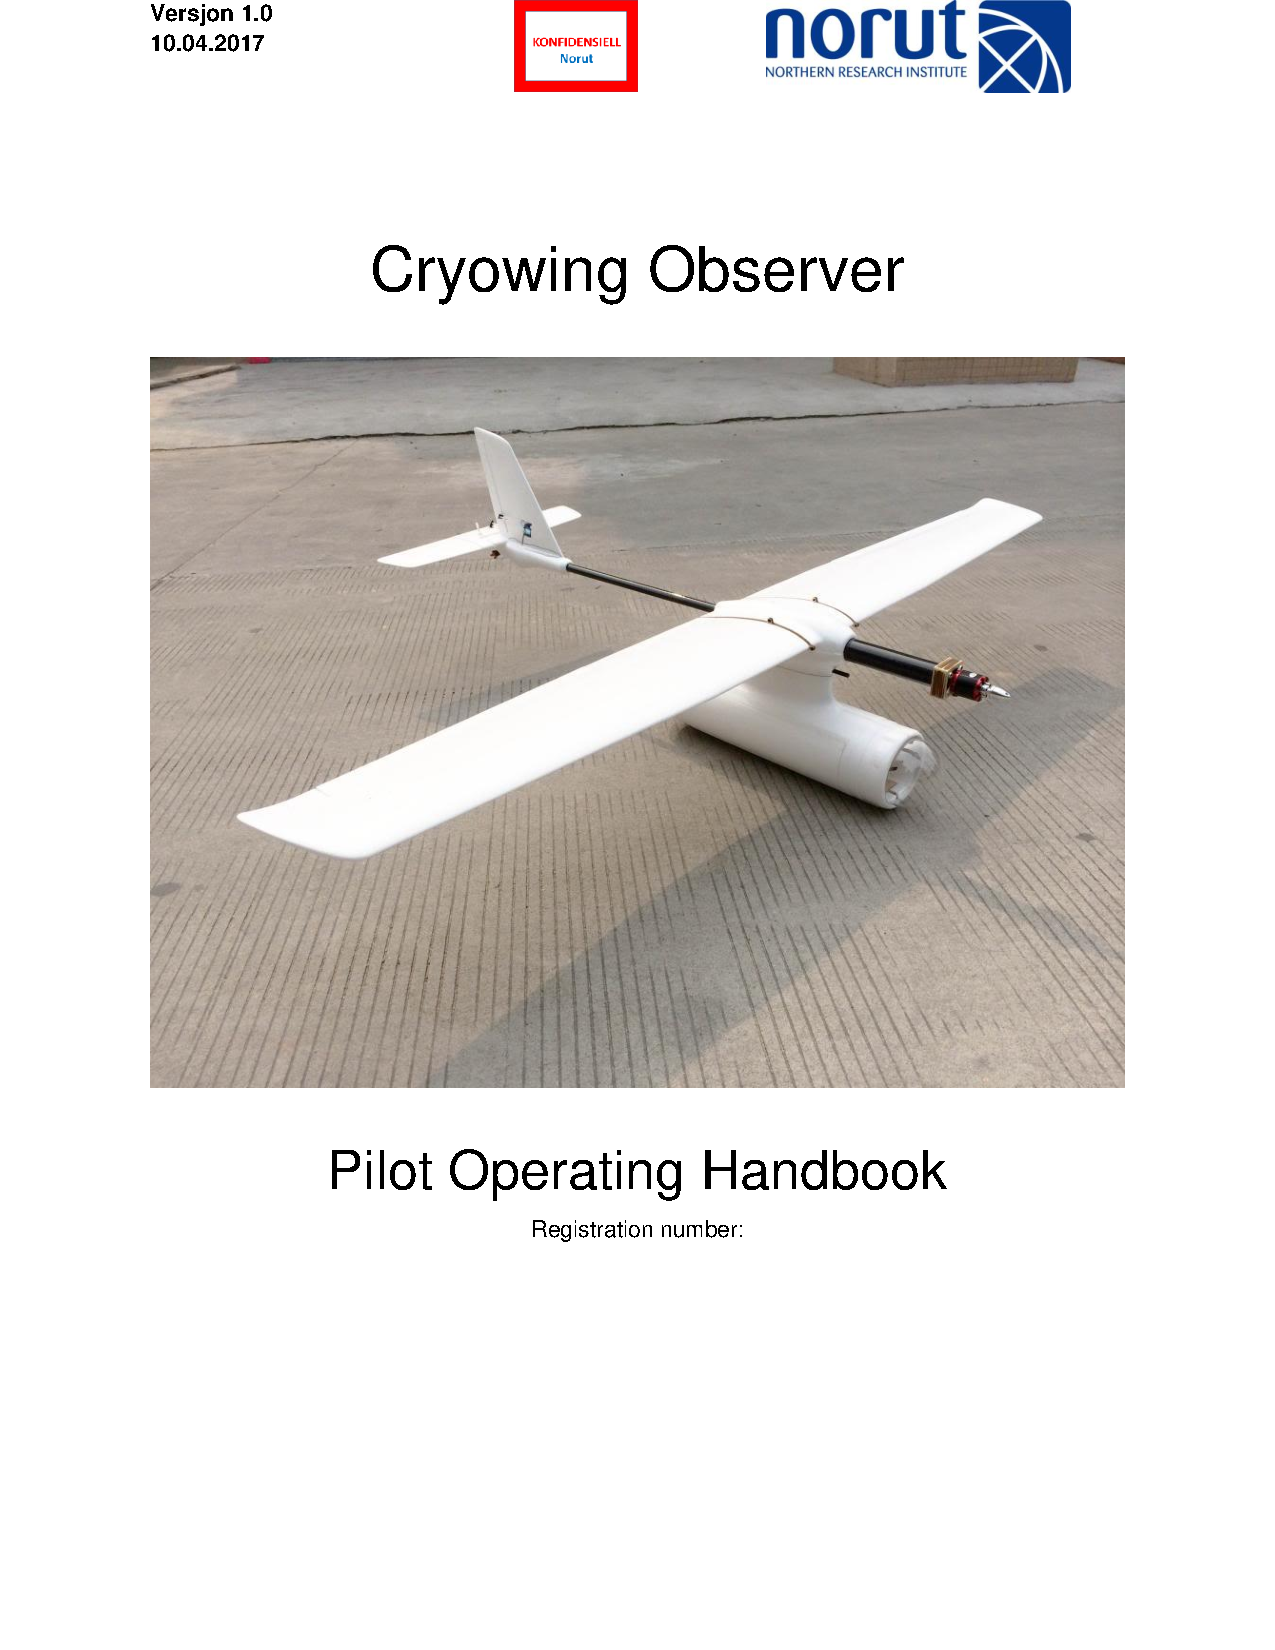
\includepdf[pages=-]{vedlegg/POH_Observer.pdf}
\end{document}